% This template was originally by R. Jacob Vogelstein
% Updated on March 1, 2010 by Noah J. Cowan


\documentclass[12pt,oneside,final]{thesis}\usepackage[]{graphicx}\usepackage[]{color}
%% maxwidth is the original width if it is less than linewidth
%% otherwise use linewidth (to make sure the graphics do not exceed the margin)
\makeatletter
\def\maxwidth{ %
  \ifdim\Gin@nat@width>\linewidth
    \linewidth
  \else
    \Gin@nat@width
  \fi
}
\makeatother

\definecolor{fgcolor}{rgb}{0.345, 0.345, 0.345}
\newcommand{\hlnum}[1]{\textcolor[rgb]{0.686,0.059,0.569}{#1}}%
\newcommand{\hlstr}[1]{\textcolor[rgb]{0.192,0.494,0.8}{#1}}%
\newcommand{\hlcom}[1]{\textcolor[rgb]{0.678,0.584,0.686}{\textit{#1}}}%
\newcommand{\hlopt}[1]{\textcolor[rgb]{0,0,0}{#1}}%
\newcommand{\hlstd}[1]{\textcolor[rgb]{0.345,0.345,0.345}{#1}}%
\newcommand{\hlkwa}[1]{\textcolor[rgb]{0.161,0.373,0.58}{\textbf{#1}}}%
\newcommand{\hlkwb}[1]{\textcolor[rgb]{0.69,0.353,0.396}{#1}}%
\newcommand{\hlkwc}[1]{\textcolor[rgb]{0.333,0.667,0.333}{#1}}%
\newcommand{\hlkwd}[1]{\textcolor[rgb]{0.737,0.353,0.396}{\textbf{#1}}}%

\usepackage{framed}
\makeatletter
\newenvironment{kframe}{%
 \def\at@end@of@kframe{}%
 \ifinner\ifhmode%
  \def\at@end@of@kframe{\end{minipage}}%
  \begin{minipage}{\columnwidth}%
 \fi\fi%
 \def\FrameCommand##1{\hskip\@totalleftmargin \hskip-\fboxsep
 \colorbox{shadecolor}{##1}\hskip-\fboxsep
     % There is no \\@totalrightmargin, so:
     \hskip-\linewidth \hskip-\@totalleftmargin \hskip\columnwidth}%
 \MakeFramed {\advance\hsize-\width
   \@totalleftmargin\z@ \linewidth\hsize
   \@setminipage}}%
 {\par\unskip\endMakeFramed%
 \at@end@of@kframe}
\makeatother

\definecolor{shadecolor}{rgb}{.97, .97, .97}
\definecolor{messagecolor}{rgb}{0, 0, 0}
\definecolor{warningcolor}{rgb}{1, 0, 1}
\definecolor{errorcolor}{rgb}{1, 0, 0}
\newenvironment{knitrout}{}{} % an empty environment to be redefined in TeX

\usepackage{alltt}

%\usepackage[utf8]{inputenc}
\usepackage{cite}

\usepackage{amssymb,amsmath,amsthm,amscd}
\usepackage{graphicx}
\usepackage{subcaption}

\usepackage{hyperref, mathrsfs, bm}
\usepackage{algorithm2e}
\usepackage{url}
\renewcommand{\thesubfigure}{}
% justifying
\usepackage{ragged2e}




\graphicspath{{./}{./graphs/}{./figures/}{./../JOFC-GraphMatch/graphs/}{./../JOFC_MatchDetect/graphs/}{./../SeededGraphMatch/graphs/}{./../DataFusion/}{./../DataFusion/graphs/}{./../DataFusion-graphmatch/graphs/}{./../VertexCorrespondence/graphs/}}

\usepackage{fixltx2e}
\usepackage{array}
% wrapfig is fragile: use sparingly
\usepackage{wrapfig} 
\usepackage{cmbright} %clean look
%\usepackage{times}  % Use this for ugly fonts
%\usepackage{ccfonts,eulervm} %Not bad looks nice for serif
\usepackage[T1]{fontenc}
\usepackage[latin1]{inputenc}

\usepackage{ogonek}
%\usepackage[garamond]{mathdesign}

\usepackage[none]{hyphenat}

\usepackage{verbatim}

\usepackage{multirow}

\usepackage{fancyhdr}    % Use nice looking headers along with the required footer page numbers   
%\usepackage[hypertex]{hyperref}
\usepackage{lscape} 
%Define the header/footer style
\pagestyle{fancy}
\fancyhf{}
\setlength{\headheight}{15pt}
\lhead{\leftmark}
\cfoot{\thepage}
\renewcommand{\headrulewidth}{0pt}
\fancypagestyle{plain}{% Redefine ``plain'' style for chapter boundaries
\fancyhf{} % clear all header and footer fields
\fancyfoot[C]{\thepage} % except the center
\renewcommand{\headrulewidth}{0pt}
\renewcommand{\footrulewidth}{0pt}}

\newtheorem{thm}{Theorem}
\newtheorem{cor}{Corollary}
\newtheorem{lem}{Lemma}
\newtheorem{defn}{Definition}

\usepackage[refpage]{nomencl}
\renewcommand{\nomname}{List of Notations}
\renewcommand*{\pagedeclaration}[1]{\unskip\dotfill\hyperpage{#1}}


\makenomenclature

\usepackage{makeidx}
\makeindex

%shorthand commands
%\DeclareMathOperator*{\argmin}{arg\,min}

\newcommand{\myred}{\color{red}}
\newcommand{\mygreen}{\color{green!50!black}}
\newcommand{\myblue}{\color{blue}}

\newcommand{\mcX}{\mathcal{X}}
\newcommand{\mcY}{\mathcal{Y}}
\newcommand{\mcG}{\mathcal{G}}
\newcommand{\mcF}{\mathcal{F}}
\newcommand{\argmax}{\ensuremath{\arg\max}}
\newcommand{\argmin}{\ensuremath{\arg\min}}
\newcommand{\logodds}{\ensuremath{\mbox{log odds}}}
\newcommand{\Pos}{\ensuremath{\mbox{Pos}}}
\newcommand{\Neg}{\ensuremath{\mbox{Neg}}}
\newcommand{\Star}{\ensuremath{\mbox{star}}}
\newcommand{\Error}{\ensuremath{\mbox{Error}}}
\newcommand{\diag}{\ensuremath{\mbox{diag}}}
\newcommand{\degrees}{\ensuremath{\mbox{degrees}}}
\newcommand{\1}{\ensuremath{\mbox{{\bf 1}}}}
\newcommand{\Real}{\mathbb{R}}
\newcommand{\iid}{\stackrel{iid}{\sim}}


\newcommand{\mA}{\mathcal{A}}
\newcommand{\mD}{\mathcal{D}}
\newcommand{\mK}{\mathcal{K}}
\newcommand{\mC}{\mathcal{C}}
\newcommand{\mM}{\mathcal{M}}
\newcommand{\mN}{\mathcal{N}}
\newcommand{\mT}{\mathcal{T}}
\newcommand{\mI}{\mathcal{I}}
\newcommand{\mX}{\mathcal{X}}
\newcommand{\mY}{\mathcal{Y}}
\newcommand{\mZ}{\mathcal{Z}}
\newcommand{\mF}{\mathcal{F}}
\newcommand{\mP}{\mathcal{P}}


\newenvironment{remark}[1][Remark]{\begin{trivlist}
\item[\hskip \labelsep {\bfseries #1}]}{\end{trivlist}}




\usepackage{animate}
%\tolerance=10000

%\makeglossary % enable the glossary
\IfFileExists{upquote.sty}{\usepackage{upquote}}{}

\begin{document}
\SweaveOpts{concordance=TRUE}





\title{Joint Optimization of Fidelity and Commensurability for Manifold Alignment and Graph Matching}
\author{Sancar Adali}
\degreemonth{January}
\degreeyear{2014} 
\dissertation
\doctorphilosophy
\copyrightnotice


% add your chapters, best way is to have separate TeX files for each chapter



%% FRONTMATTER
\begin{frontmatter}

% generate title
\maketitle

\begin{abstract}

Abstract goes here.

\vspace{1cm}

\noindent Primary Reader: Carey E Priebe\\
Secondary Reader: Daniel E Fishkind

\end{abstract}

\begin{acknowledgment}

Thanks!

\end{acknowledgment}

\begin{dedication}
 
This thesis is dedicated to myself who did all the hard work, my mother 

\end{dedication}

% generate table of contents
\tableofcontents

% generate list of tables
\listoftables

% generate list of figures
\listoffigures


\printnomenclature

\end{frontmatter}




\chapter{Introduction}
\label{sec:intro}
\chaptermark{Introduction:  Matched Data and Data Fusion}


In this thesis, we will investigate how to carry out inference in  data  settings where the data consist of different modalities or views. Efficient use of the data require some sort of information fusion in order to avoid the curse of the dimensionality. We are interested in what kind of information is essential for the inference task and if there exist principles that one should keep to for acceptable performancein the task. We are also interested in exploring how these  queries and their answers are  relevant to  particular data problems.

\section{Data Settings}


 It is a challenge  to do a tractable analysis on data from disparate sources of data (such as multiple sensors). The increasing multitude  of sensors technology and large numbers of sensors both are  sources of difficulty and hold promise for efficient inference. One of our contributions is developing well-defined simple settings that provided intuition for the right approaches to data fusion and which led to practically useful inference methods.
 
 
\begin{figure}
\centering
\includegraphics[scale=0.75]{gen-model-orig-proj.pdf}
\caption{Multiple Sensor setting \label{fig:gen-model}}
\end{figure}

 Our world-view for data fusion of multiple sensors is depicted in \autoref{fig:gen-model}.


It is assumed some objects lie in some ``object'' space $\Xi$, and each sensor has another ``view'' of the objects. The measurements recorded by the $i^{th}$ sensor lie in some ``measurement space'' $\Xi_i$. The usual approach in pattern recognition is to use feature extractors on the spaces to get a feature representation in Euclidean space and use classical pattern recognition tools to carry out the exploitation task. The alternative approach is to acquire dissimilarities between the group of objects, and use the dissimilarities to either find an embedding in a low-dimensional Euclidean space where classic statistical tools are available for inference or use dissimilarity-based versions of pattern recognition tools~\cite{duin2005dissimilarity}. The embedding approach in a  low-dimensional Euclidean space will be used where the small number of embedding dimension allow us to avoid ``curse of dimensionality''. Also, the embeddings of dissimilarities from  different conditions will be required to be ``commensurate'' so that sensor measurements can be compared or jointly used in inference. This is accomplished by maps $\rho_k,k=1,\ldots,K$ from measurement spaces $\Xi_k$ to a low-dimensional commensurate space $\mathcal{X}$ visualized in \autoref{fig:gen-model}. Learning these maps from data is  an important portion of our novel  approach.
\label{sec:data}

\subsection{Exploitation Task}
Data fusion is a very general concept and the specific meaning of data fusion and the setting we have in mind should be clarified here. The exploitation task we are interested in might involve (perhaps notional) complex objects or abstract entities that are not practically representable. The objects are members of a (perhaps notional) space called ``object'' space, $\Xi$ in Figure \ref{fig:gen-model} . We will have different ``views'', ``measurements'' or ``data modalities'' extracted from these objects (which we will refer to as ``conditions''), and these observations will be elements of the measurement space for those ``conditions'' ($\Xi_k$ for $k^{th}$ condition). Each example of the objects will have an observation in each of the different conditions and the corresponding observations across different ``conditions'' will be ``matched''. Given new observations from these different ``conditions'', is it possible to decide if they are "matched``? Or if a group of  observations from each condition are ``matched'' to each other, but the specific correspondences are unknown, is it possible to find the true correspondences? Different approaches are proposed in this dissertation to address these questions.
\label{subsec:task}



\section{Dissimilarity representation\label{sec:dissim_repr}}
 Great progress been made in the theory and applications of pattern recognition, particularly in problem settings where the data available or assumed to be available as vectors in metric spaces. There are still many problems where due to the nature of setting, one only has access to dissimilarities or  proximities or distances between measurements or subjective assessment  of similarities of objects. Thus, we have a superficial distinction between these two kinds of settings, even though the inference task is agnostic about this representation issue. The gap between the two kinds of representation of data can be bridged using various  techniques, such as different kinds of embedding methods and computing dissimilarities between entities.
We will refer to the entities of interest for pattern recognition as objects. These might be real objects or abstract concepts. The data will be a collection of measurements for instances or examples of these objects.
 \cite{duin2005dissimilarity} is an excellent resource that compiles the fruits of research in learning from  dissimilarity-based representation. In the introduction, the authors make clear the distinction between statistical and structural(syntactic) pattern recognition, which is previously discussed in \cite{NadlerSmith1993}. The first is concerned with the analysis of features which are lists of measured values for object attributes. The second uses a relational view of objects for representation. In both cases,  the task of discrimination  can rely on distances (however they are defined). P\k{e}kalska and Duin  suggest dissimilarity measures  are a natural bridge between these two types of information and this applicability to  multiple settings motivates our use of dissimilarity representation in information fusion. 
For feature-based representation, one first defines the features which are either raw or processed measurements from sensors observing the objects and  represention of each object is a single point in the representation space. Dissimilarity-based representation relies on a dissimilarity measure, a way of quantifying the dissimilarity, proximity or similarity between any two objects. It is quite possible, in fact preferable, that the dissimilarity is \emph{designed for} the inference task at hand. 
%\cite{Duin} argue this is a reason dissimilarities can be superior, since similarities can encode concepts of class membership directly in class discrimination problems.
There are naturally multiple ways (some more natural than others) of comparing entities and this fact will provide one of the arguments for our approach to information fusion from  data sources, even sources that collect  data of same modality. In  the latter case where the data comes from separate sensors that are of the same type, the same measurements might have different dissimilarity representation according to subjective judgments or different dissimilarity  measures. 

\section{Match Detection}

We will now provide a formal description of the problem that was the initial motivation for our investigations, along with a few general remarks. We will go into more detail in  \ref{chap:match_detection}.

Consider $n$  distinct objects, which are described with finite number of measurements. Each of the measurements $x_{ik}$ lies in  the corresponding space $\Xi_k$ and the  measurements $x_{ik}$ are matched for the same $k$ index
\[  \begin{array}{cccc}
        & \Xi_1 & \cdots & \Xi_K\\
        Object ~ 1 & \bm{x}_{11} & \sim \cdots \sim & \bm{x}_{1K} \\
        \vdots & \vdots & \vdots & \vdots \\
        %\text{Object} ~ i & \bm{x}_{i1} & \sim \cdots \sim & \bm{x}_{iK} \\
        %\vdots & \vdots & \vdots & \vdots \\
        Object ~ n & \bm{x}_{n1} & \sim \cdots \sim & \bm{x}_{nK}
      \end{array}      
\]
To each pair of measurements $x_{ik},x_{jk}$ in the same space, we can assign a dissimilarity value $\delta_{ijk}=\delta\{x_{ik},x_{jk}\}$, possibly dependent on the space $\Xi_k$. We assume the dissimilarities to be non-negative and  symmetric, and 0 for $\delta\{x_{ik},x_{ik}\}$.  It is this training set of  dissimilarities we utilize to do inference on the following exploitation task:

 Given dissimilarities between  $K$ new measurements/observations ($\bm{y}_{k};k=1,\ldots,K$) and the previous $n$ objects under $K$ conditions, 
test the null hypothesis  that ``these measurements are from the same  object"  against the alternative hypothesis that ``they are not  from the same  object"~\cite{JOFC}:
    \[
\begin{array}{l}
%\hspace{-2em}
    H_0: \bm{y}_{1} \sim \bm{y}_{2} \sim \cdots \sim \bm{y}_{K}
 \text{ versus } 
 H_A: \exists i, j , 1\leq i < j \leq K :\bm{y}_{i} \nsim \bm{y}_{j}  
\end{array}
\]
 The null hypothesis can be restated as the case where the dissimilarities are ``matched" and the alternative as the case where they are not ``matched".

We represent the dissimilarities in the form  of $n \times n$  dissimilarity matrices $\{\Delta_k;k=1,\ldots,K\}$ with entries $\{\delta_{ijk} ;  i=1,\ldots,n;\quad j=1,\ldots,n\}$  and a  vector (of length $nK$) of dissimilarities  $\mathbf{\Delta}^{new}=\{ \delta_{ik}^{new}; i=1,\ldots, n;\quad k=1,\ldots,K\}  $  where $\delta_{ik}^{new} $ is the dissimilarity  between  $x_{ik}$ and $y_k$.
 
 
For the hypothesis testing problem, we need to compute the test statistics for the objects represented by the given dissimilarities. So what is needed is to find a collection of mappings (one from each ``condition'') to a lower dimensional space where new observations from each condition can be mapped to be made commensurate. These mappings does not need to be  well-defined; they can be the results of embedding routines for a particular dataset. As long as the embedding of the dissimilarity results in a  unique mapping,  out-of-sample embeddings could be adjoined to the embedding of in-sample dissimilarities.

A few points should be mentioned to distinguish our approach from related approaches and accentuate the specific challenges of the inference task.
\begin{remark}
Due to the fact that data sources are ``disparate", it is not immediately obvious how  a dissimilarity between an object in one condition and another object in another condition  can be computed, or even defined.  In general, these between-condition between-object  similarities are not available.
\label{rem:between_cond_diss}
\end{remark}
 
 \begin{remark}
 Whether the data is collected in dissimilarity representation for each condition, or whether dissimilarities are computed for the observations which are feature observations at each condition is not relevant to our exploitation task: it is assumed one way or another (perhaps from experts in the domain of the problem),  dissimilarities for each condition are available for inference purposes. 
\end{remark}

\begin{remark}
The exploitation task  being considered is \emph{not} accurate reconstruction of these feature observations, even if they do exist. The quality of the  embeddings need to just be  good enough to be useful in the inference task. Therefore, the quality of our representation will be dependent on the bias-variance tradeoff, where by choosing a low-dimensional representation, we might be introducing more model bias, but the representation will be more  robust with respect to noise and might result in smaller error in the inference task.
\end{remark}

We will make use of this inference problem for elucidating two concepts that we introduce  in \ref{chap:FidComm}. Our novel solution to this matching problem will use those concepts as two criteria for finding the mappings from each ``condition'' to the common low-dimensional space.




\chapter{Related Work}
\label{chap:RelatedWork}
\chaptermark{Related Work}



\section{Multiple View Learning}
\label{sec:MultiViewLearn}
When data are collected using a multitude of sensors or under significantly different environmental conditions, we refer to  the data setting as a multiple view setting where each ``view'' provide possibly complementary  information about the observed objects\footnote{We use the term ``object''  loosely, as the observed objects could be topics or concepts and the  collected data could be text, images, etc.}. Multiple view learning seeks to exploit these views simultaneously to be more successful in the learning task.

In data settings for multiview learning, the data consist of observations from $K>1$ views, where both the relationship between the attributes from different views and the relationship between the features and the quantity to be predicted are unknown. The objective is to train the best predictor. While it is possible to use all the attributes in different views and carry out feature selection without regards from which view they come from, this ignores the fact that the modalities can be quite diverse and combining features from different modalities is not always meaningful. Consider features extracted from an image  and an audio segment as features from different modalities. A classifier that treats these features in the same way without taking into consideration their modalities is  unlikely to have good performance.
It is more reasonable to use the prior information that the features in the same modality are much more likely to be correlated or commensurate with each other than features in different views and use predictors more suited to each modality, if the different modalities are diverse.

 Multiple View Learning is a burgeoning field, as there are many cases where one has to leverage many different related datasets for an inference task. For example, for learning  tasks related to webpages (such as webpage categorization, ranking of relevant webpages) both content of the webpages and the hyperlink structure between the webpages can be used. For social networks, people have different relationships with other people in their networks: networks  may be based on similarity of interests, geographical proximity, job relationships, etc. Combining information from different social networks would provide a more complete look into underlying social life of the people in the network and one would expect better performance in for all kinds of  inference based the social network data.

In addition, when it is necessary to collect more data, in a lot of cases it is easier to collect data in different modalities, than it is to collect more samples in a single modality. For example in medical studies, it is much easier to  collect medical data from already recruited patients, compared to recruiting new patients. Data from different modalities might provide complementary information and could result in much more effective predictors, as opposed to data from a single modality that provides diminishing returns with increasing sample size.

There are  also connections of this topic to well-studied machine learning subjects such as dimensionality reduction. As more data is collected, it is necessary to learn a low-dimensional representation of the data to avoid the curse of dimensionality. An interesting question is how to carry out dimensionality reduction in a multiple view setting: is it better to do dimensionality reduction separately for each modality, and concatenate the resulting low-dimensional representations, or find a joint low-dimensional representation  for all of the modalities? This is a question we try to answer for data settings we discuss in this thesis.

In the case of missing data, observations of features in the same view could  be missing altogether. In the case of such structurally missing data, it makes sense to learn predictors that use features from different views independently, so that a predictor could make an accurate prediction even if observations from some of the views are missing.


In  \cite{Amini2009}, the authors  discuss  an example of multiview learning problems, classification of a multi-lingual document corpus. They  co-train  classifiers for single-language data that jointly minimize  loss in each single language along with disagreement between classifiers on training examples. Their findings support the intuition that  classifiers which are based on multiview learning preform than those classifiers who have been trained with only data from a single view.

In \cite{Sun2005}, features
are fused via CCA to have better classification performance compared to the original set of features in a typical classification problem.

A popular approach to multiview learning is learning a  kernel matrix for each modality and combining these kernels in an optimal way (with respect to the inference task). For $K$ views, let $i^{th}$ datum for $k^{th}$ be represented $X_{ik},\quad i \in {1,\ldots n}, k \in \{ 1,\ldots, K \}$ . For the datum in the same view, let ${\mcK}_{k} = \left[ \mck_{k} (X_{ik},X_{jk}) \right] $ be the kernel matrix defined for that view.  Since any convex combination of the kernels $\sum{\alpha_k \mck_{k} } $ is also a kernel, it is possible to compute a joint kernel $\mck$ that use all of the multiview data by convexly combining this data. Assuming that a kernel can be defined for each view, the learning problem is  finding the optimal (for the inference task) coefficients $\alpha_k$ for each view. These parameters are usually estimated using training data. Denoting the optimal  $\alpha_k$ by  $\hat{\alpha}_k$,  $\hat{\mcK} = \sum_k{\hat{\alpha}_k \mcK_{k} }  =  \left[ \sum_k{\hat{\alpha}_k {\mck_k} (X_{ik},X_{jk})} \right] $.  Given a new datum $x$, the kernel function for each view, $\mck_{k}$ ,  along with $\hat{\alpha}_k$ is used to compute the inner product for the joint kernel. 
\[
{\mck}(x,.)= \sum{\hat{\alpha}_k {\mck_k} (x_{k},X_{ik})} 
\]

Many papers on ``Multiple Kernel Learning"   exist in the literature~\cite{McFee:2011:LMS:1953048.1953063,Lin2009,Lanckriet2004} which are reviewed in a comprehensive survey \cite{MKLSurvey}.
Choi et al.\ \cite{Choi:2008:MIM:1619995.1620064} use the Markov random walk interpretation of multiple kernel matrices to combine into one kernel matrix. \cite{ZhouBurges2007a} is another work that uses the random walk interpretation to deal with multiview data. The learning task in  \cite{ZhouBurges2007a} is spectral clustering with multiple graphs.

\section[Transfer Learning and Domain Adaptation]{Transfer Learning \label{sec:translearn}}

Methods which utilize training data in one domain  as auxiliary information for  learning  in another domain fall under the term ``transfer learning'' \cite{TransLearnSurvey}. Sometimes the source domain and the target domain are actually the same, but the distribution of the data is different , e.g. inherent difference between training and test data due to collection conditions. We call this phenomenon sample selection bias or covariance shift (SSB/CS) \cite{Zadrozny2004a,TransLearnSurvey}.

According to \cite{Hand2006}, this SSB/CS phenomenon is common in real life data analysis problems, and is usually understated by practitioners. For evaluation of newly designed classifiers, the classifiers are trained on a portion of the available data and tested on the held out data, so when evaluating classifiers, the assumption that training and test data come from the same distribution is usually valid. However any performance improvements that a new classifier model has over baseline would be swamped  by the sample selection bias. Thus, one should be skeptic about improving accuracy scores for benchmark datasets in machine learning and seeing them as evidence of progress.

Let us clarify the differences between transfer learning  and SSB/CS.  Let $y$ denote the random variable for the class label  for classification or the dependent variable for regression and $X$ denote the random variates we will use for the learning task. We will  make use of  the common assumption that data is $\iid$.  
Suppose we have two domains  ${\mcD}_s$ and ${\mcD}_t$ where the training data and test data is collected from, respectively. These are called the source and target domains, respectively.
The training data $\left(X_i,y_i\right) \in {\mcD}_s$ and are drawn from the joint distribution $\Pry(X,y)$. 
The test data $\left({X'}_i,{y'}_i\right) \in {\mcD}_t$ and have the distribution $\Pry'(X,y)$.
The most general objective is to infer $\Pry'(X,y)$  given $\iid$ sample of $\left(X_i,y_i\right) \in {\mcD}_s$. 
The learning task is usually minimizing  $\argmin E[\ell\{y, \argmax_y{\hat{\Pry}'(y \| X) } \}]$  
where $\hat{\Pry}'(y \| X)$  is an approximation  $\Pry'(X,y)$ based on the training and the test data. Basically we require an inference method for the data distribution of the target domain   $\hat{\Pry}'(y \| X)$ that minimizes expected loss for prediction in the target domain.

In the classical supervised learning setting, the source and target domains are the same and  $\Pry(X,y)$ is assumed to be the same as $\Pry'(X,y)$. If the target domain is the same as the source domain, ${\mcD}_s={\mcD}_t=\mcD$, but $\Pry(X) \neq\Pry'(X)$ while $\Pry(y\|X) \approx \Pry'(y \| X)$, this is the \emph{covariate shift} problem.  When we cannot make either of the assumptions $\Pry(X) = \Pry'(X)$ or $\Pry(y\|X) = \Pry'(y \| X)$, we have the \emph{sample selection bias} problem \cite{Zadrozny2004a}.


 In some learning problems, the source and target domains are different ${\mcD}_s \neq {\mcD}_t$ and all or a considerable portion of  the labels $\{{y'}_i\}$  in $\left({X'}_i,{y'}_i\right) \in {\mcD}_t$ are missing. In this case, domain adaptation methods allow the exploitation of both the  data in the source domain $\{\left({X}_i,{y}_i\right)\}$ and the data in the target domain  $\{\left({X'}_i,.\right)\}$ to construct a good predictor for the target domain\cite{DaumeIII2006,Ben-David_Dom_Adapt2007,Ling2008,Pan2008a}.
Various ``domain adaptation'' approaches\cite{Pan2008a,LowRankSharedConceptChen2012a} assume existence of mappings to a common latent space ${\mcD}_{com}$,  $\Psi_s:{\mcD}_s \rightarrow {\mcD}_{com} $ and $\Psi_t:{\mcD}_t \rightarrow {\mcD}_{com}$ to a  such that the class conditional distributions $\Pry(\Psi_s(X) \|y) \approx \Pry(\Psi_t(X') \| y'=y)$.  If these mappings to the commensurate space can be inferred, then they can be used to predict $y'$ given $\Psi_t(X')$ even if no $\left({X'}_i,{y'}_i\right) \in {\mcD}_t$ pairs exist. 
%Other approaches infer a mapping from from the source domain to the target domain.
In {Pan2008a}, for example, the distance between the conditional distributions $\Pry(\Psi_s(X) \|y) $ $\Pry(\Psi_t(X') \| y'=y)$ is computed via  Maximum Mean Discrepancy
measure and  the mappings $\Psi_s$ and  $\Psi_t$  are inferred by the minimization of MMD measure.

\section[Manifold Matching]{Manifold Alignment}
There have many efforts toward solving ``manifold alignment", which is a problem related to both our data fusion problem, and the transfer learning problem\ref{sec:translearn}. ``Manifold alignment" seeks to find correspondences between observations from different ``conditions". The setting that is most similar to ours is the semi-supervised setting, where a set of correspondences are given and the task is to find correspondences between a new set of points in each condition. In contrast, our hypothesis testing task is to determine whether any given pair of points is ``matched" or not. The proposed solutions follow a common approach in that they look for a common commensurate space such that the representations (possibly projections or embeddings) of the observations in the commensurate space match.

Note the similarity of the  description of ``manifold alignment''   to the latent space approach for domain adaptation. For both domain adaptation and manifold alignment, the objective is to find mappings to a  common space  so that the data in  one domain can be used for inference in the other domain.

Wang and Mahedavan~\cite{Wang2008} suggest an  approach that uses embedding followed by Procrustes Analysis to find a map to a commensurate space. Given a paired set of points, Procrustes Analysis~\cite{Sibson}, finds a transformation from one set of points to another in the same space that minimizes sum of squared distances, subject to some constraints on the transformation. In the case mentioned in \cite{Wang2008}, the paired set of points are corresponding low-dimensional embeddings of kernel matrices.   For the embedding step, they made the choice of using Laplacian Eigenmaps, though their algorithm allows for any appropriate embedding method.

 Zhai et al.~\cite{Zhai2010}  finds two projection matrices to minimize three terms in an energy function similar to our JOFC approach (see chapter \ref{chap:FidComm}). One of the terms is the \emph{correspondence preserving term} which is the sum of the squared distances between corresponding points and is analogous to our commensurability error term. The other two terms are \emph{manifold regularization terms} and consist of the reconstruction error for a Locally Linear Embedding of the projected points. These terms, analogous to fidelity, make sure the projections in the lower dimension retain the structure of the original points. For fidelity error terms in our setting, this is done by preserving dissimilarities. For manifold regularization terms, this is done by preserving the local neighborhood of points, such that close points are not mapped apart.
Ham and Lee\cite{HamLee2005a} solve the problem in semi-supervised setting by a similar approach, by minimizing a cost function of three terms, two terms for fidelity of embedding, one term of commensurability.
In another paper  the simultaneous embedding is written  as a single function  that combines Fidelity and Commensurability terms. By using Local Linear embedding,  they are able to formulate the embedding as a function of a $2n \times d$ configuration matrix, and a tradeoff parameter between \emph{inter-dataset} and \emph{intra-dataset error} (corresponding to commensurability and fidelity, respectively). This approach could be used as another tool for the investigation of JOFC.



Another approach is Three-way Multidimensional scaling\cite{3wayNMDS,borg+groenen:1997}.
 This approach assumes the  different ``conditions" of the data are linear transformations of a single configuration and aims to find this single configuration and the linear transformation. With this approach, the mappings  $\{\rho_k \}$ that we define in \autoref{fig:gen-model} and \autoref{sec:data} are  assumed to be embeddings followed by linear transformations. See also \autoref{subsec:3wayMDS}.
 %For our setting, one would first embed the in-sample dissimilarities via the three-way MDS, which would give as the linear transformations that map from group configuration to individual configurations under each condition. This is followed by out-of-embedding the OOS dissimilarities, and use the inverse of the transformation matrices to find the out-of-sample embeddings with respect to the group configuration. Since the out-of-sample embeddings are commensurate, the test statistic can be computed as the distance between the OOS embeddings. 




\chapter{Multidimensional Scaling,Its Variants and Principal Components Analysis}
\label{sec:MDS}
\chaptermark{Multidimensional Scaling and Its Variants}



\section{Multidimensional Scaling}
Multidimensional Scaling (MDS) is the general term used to describe methods to  ~\cite{CMDS,borg+groenen:1997,duin2005dissimilarity}  embed dissimilarities in the Euclidean space  with a chosen dimension $d$ such that the distances between the embeddings are as close as possible (in various senses) to the original dissimilarities. Different criterion functions can be used to measure how close the distances are  to the given dissimilarities, leading to different embedded configurations. These different variants of MDS can be described using a single formulation which will be introduced in \autoref{sec:MDSvariant}.

Consider a  set of n objects. For each pair of objects, the dissimilarity value, denoted by $d_{ij}$ is a non-negative real number which quantifies how dissimilar those two objects are. The collection of these values form the matrix $\Delta$ , which is  a $nxn$ dissimilarity matrix. %While, in general, dissimilarities between finite set of objects are being considered; for a dissimilarity matrix, we can consider the objects as points in a space, whose neighborhood relationships are defined by the dissimilarity measure.
The dissimilarities have to satisfy $\delta_{ij}\geq 0$ and $\delta_{ii}=0$ and $d_{ij}=d_{ij}$. Therefore  $\Delta$ is non-negative, hollow and symmetric. If, in addition, each triplet of dissimilarities $\delta_{ij}$, $\delta_{ik}$ and $\delta_{ik}$  satisfy the triangle inequality, then D is called  an Euclidean distance matrix.


\section{Different criterion for MDS \label{sec:MDSvariant}}
Multidimensional Scaling finds a configuration of points consistent with given dissimilarities in a finite dimensional Euclidean space. There are various variants of MDS that use different measures of consistency.  In general, the criteria minimize discrepancy between $f(\delta_ij)$ and  $d(\bm{x_i},\bm{x_j})$ where $d(\cdot,\cdot)$ is the Euclidean distance function and $f(\cdot)$ is monotonically increasing function. Depending on whether ``metric" or ``non-metric" MDS is being considered, $f(\cdot)$ is either a linear transformation or a non-linear one. Specific variants of MDS are defined by $f(\cdot)$ and the measure of discrepancy between  $f(\cdot)$ and $d(\cdot,\cdot)$. We call the latter \emph{the criterion function} which is optimized with respect to the embedding coordinates.


\subsection{Metric MDS}
 For metric MDS, transformations of the form  $f(x)=ax+b$ are allowed.
 \subsubsection{Stress Criterion}
 Setting $f(x)=x$ and choosing  the discrepancy measure between the dissimilarities and distances of embedded points to be $\ell_2$, the resulting criterion is called the raw stress criterion. Additionally weights ($w_{st}$) can be introduced for each discrepancy term. Denoting the matrix composed of the weights by $W$, we write
 \begin{equation}
\sigma_{W}(X)=\sum_{1\leq s\leq n;1\leq t\leq n} {w_{st}(d_{st}(X)-\delta_{st})^2  }\label{raw-stress}
\end{equation}
Subtypes of Stress criterion is identified by different choices for $w_st$ which depend on the original dissimilarities $\delta_{st}$ .
For example, choosing $w_{st}=\left[{\sum{\delta_{st}^2}}\right]^{-1}$ normalizes the stress so that the stress value is always between 0 and 1. One can compare different configurations by this standardized stress value and conclude whether a configuration is a good fit or not based on this value.

A slightly different weighting scheme is $w_{st}=\left[ \sum_{st}{\delta_{st}-\bar{\delta} } \right]^{-1}$ 
where $\bar{\delta}=\frac{1}{(n)(n-1)} \sum_{st}{\delta_{st}}$ (average of dissimilarities).

Another related criterion is SSTRESS criterion which involves squares of dissimilarities and distances:
\[
=\sum_{s,1\leq s\leq n}\sum_{t;1\leq t\leq n} { \left(d_{st}^2(X)-\delta_{st}^2\right)^2  }
\]


\subsubsection{Sammon Mapping Criterion}
This is a specific case of the Stress criterion where the weights $w_{st}$ are set to be $\delta_{st}^{-1} \left[\sum_{k<l}\delta_{kl} \right]^{-1}$. These set of weights normalizes the squared discrepancies in the stress criterion by the magnitude of the original dissimilarities, so that discrepancy terms for the larger dissimilarities do not dominate the optimization of the criterion function. As a result, small $\delta_{st}$ are preserved just as well as large $\delta_{st}$.

\subsection{Ordinal (Nonmetric) MDS}
 For Nonmetric MDS, $f(\cdot)$    is allowed to be  any monotonic transformation. Specifically in psychometric applications of MDS, the assumption that the dissimilarities are a scaled-shifted version of the ``true"  dissimilarity is an unwarranted assumption. It is possible the existence of a ``true" dissimilarity is in question. Even if the dissimilarities are physical distances, humans tend to have biased estimates of those distances (long distances are usually underestimated ). \cite{Trosset1998}. This variant of MDS is also called ordinal, because what is preserved is the rank of dissimilarities, not their magnitude.

\subsection{Classical MDS and the Strain Criterion}

An $n \times n$ matrix $\Delta = \left[\delta_{st}\right]$ is a distance matrix iff it is symmetric and $\delta_{ii}=0$ $\delta_{st} \geq 0 \onespace \forall s,t$ and if it obeys the triangle inequality $\delta_{sr}+\delta_{rt} \geq \delta_{st}$ for any triple $s,r,t$.

$\Delta$ is Euclidean if there exist a configuration of points $\bm{x}_{i} \in \mathbf{R}^d$ such that for any pair $s,t \in \{1,\ldots,n\}$,    $\delta_{st}=d(\bm{x}_{s},\bm{x}_{t})$.

Consider the case where $\Delta$ is Euclidean. Note that if $\bm{x}_{i},i \in \{1,\ldots,n\} $ satisfy $\delta_{st}=d(\bm{x}_{s},\bm{x}_{t})$ for any pair $s,t$, for any constant vector $\bm{u}$ and any rotation/reflection matrix $R$, the same group  of points transformed by $R$ and   $\bm{u}$ $R\bm{x}_{i}+\bm{u}$ . To remove the translational ambiguity, set   $\sum{\bm{x}_{i}}$  to $\bm{0}$. How could we recover the original configuration   $\{\bm{x}_{i}\}$ from $\Delta$ (perhaps up to rotation/reflection)?
The relation between the entries of $\Delta$ and $\bm{x}_{i}$ can be written as
\[
\delta_{st}^2= d(\bm{x}_{s},\bm{x}_{t})^2 = \|\bm{x}_{s}   \|^2 +   \|\bm{x}_{t}   \|^2   -   2  \bm{x}_{s} \cdot  \bm{x}_{t}   
\label{eq:diss_wrt_embed_coords}
\]
Summing \eqref{eq:diss_wrt_embed_coords} over $s$, over $t$ and then over $s$ and $t$, we get the following identities
\begin{align}
\label{eq:diss_wrt_embed_coords_2_1}
\sum_s{ \delta_{st}^2} &= \sum_s{\| \bm{x}_{s}   \|^2} + n \|\bm{x}_{t}   \|^2 -2 \sum_s{ \bm{x}_{s}   \cdot\bm{x}_{t}    } \quad s=1,\ldots,n\\
\label{eq:diss_wrt_embed_coords_2_2}
\sum_t{ \delta_{st}^2} &= \sum_t{\| \bm{x}_{t}   \|^2} + n\|\bm{x}_{s}   \|^2  -2 \sum_t{ \bm{x}_{s}   \cdot\bm{x}_{t}   } \quad t=1,\ldots,n \\
\label{eq:diss_wrt_embed_coords_2_3}
\sum_{st}{ \delta_{st}^2} &= 2n\sum_{t}{\| \bm{x}_{t}   \|^2}  -2\sum_{s}{ \bm{x}_{s} } \cdot \sum_t{   \bm{x}_{t} }
\end{align}
.

Dividing each equality by $\frac{1}{n}$ , $\frac{1}{n}$ and $\frac{1}{n^2}$ respectively and using the fact that $\sum{\bm{x}_{i}}=\bm{0}$,
\begin{align}
\label{eq:diss_wrt_embed_coords_3_1}
\frac{1}{n}\sum_s{ \delta_{st}^2} &= \frac{1}{n}\sum_s{\|\bm{x}_{s}   \|^2 } +  \|\bm{x}_{t}   \|^2 \quad   t=1,\ldots,n\\
\label{eq:diss_wrt_embed_coords_3_2}
\frac{1}{n}\sum_t{ \delta_{st}^2} &= \frac{1}{n}\sum_t{\|\bm{x}_{t}   \|^2 }+  \|\bm{x}_{s}   \|^2 \quad   s=1,\ldots,n\\
\label{eq:diss_wrt_embed_coords_3_3}
\frac{1}{n^2}\sum_{st}{ \delta_{st}^2} &= \frac{2}{n}\sum_{t}{\|\bm{x}_{t}   \|^2} 
\end{align}

Reorganizing terms, we get
\begin{align}
\label{eq:diss_wrt_embed_coords_4_1}
\|\bm{x}_{t}   \|^2  &= \frac{1}{n}\sum_s{ \delta_{st}^2} + \frac{1}{n}\sum_s{\|\bm{x}_{s}   \|^2   } \\
\label{eq:diss_wrt_embed_coords_4_2}
\|\bm{x}_{s}   \|^2  &= \frac{1}{n}\sum_t{ \delta_{st}^2} + \frac{1}{n}\sum_t{\|\bm{x}_{t}   \|^2  }\\
\label{eq:diss_wrt_embed_coords_4_3}
0 &= -\frac{2}{n}\sum_{t}{\|\bm{x}_{t}   \|^2} +\frac{1}{n^2}\sum_{st}{ \delta_{st}^2} 
\end{align} .


Summing the three equations 
\eqref{eq:diss_wrt_embed_coords_4_1}, \eqref{eq:diss_wrt_embed_coords_4_2}  and  \eqref{eq:diss_wrt_embed_coords_4_3} and replacing   $\|\bm{x}_{s}   \|^2 +\|\bm{x}_{t}\|^2$  in the original equation \eqref{eq:diss_wrt_embed_coords} with this sum, we get 

\[
\delta_{st}^2= \frac{1}{n}\sum_s{ \delta_{st}^2} + \frac{1}{n}\sum_s{\|\bm{x}_{s}}   \|^2 + \frac{1}{n}\sum_t{ \delta_{st}^2} + \frac{1}{n}\sum_t{\|\bm{x}_{t}}  \|^2  -\frac{2}{n}\sum_{t}{\|\bm{x}_{t}   \|^2} +\frac{1}{n^2}\sum_{st}{ \delta_{st}^2}   -2\bm{x}_{s}   \bm{x}_{t}  
\].

After simplification, we get
\[
\delta_{st}^2= \frac{1}{n}\sum_s{ \delta_{st}^2} +  \frac{1}{n}\sum_t{ \delta_{st}^2}  +\frac{1}{n^2}\sum_{st}{ \delta_{st}^2}  -2\bm{x}_{s}   \bm{x}_{t}   
\]

Rearranging terms, we get the dot product of $\bm{x}_{s}$ and $\bm{x}_{t}$ :
\[
\bm{x}_{s}   \bm{x}_{t} = \frac{-1}{2} \{\delta_{st}^2 - \frac{1}{n}\sum_s{ \delta_{st}^2} -  \frac{1}{n}\sum_t{ \delta_{st}^2}  +\frac{1}{n^2}\sum_{st}{ \delta_{st}^2 }     \| \}
\]



Some of the sums in the above expression can be written in matrix notation
\begin{align*}
\bm{1}^{T}\Delta^2= \frac{1}{n}\sum_s{ \delta_{st}^2}\\
\Delta^2 \bm{1} = \frac{1}{n}\sum_t{ \delta_{st}^2}
\end{align*}.

Using the above expressions and placing $\{\bm{x_i}\}$ rowwise into an $n \times d$ matrix $X$, we can write all of the terms in matrix notation
\begin{align*}
XX^T = \frac{-1}{2} \{\Delta^2 -  \frac{1}{n} \bm{1}\bm{1}^{T}\Delta^2  -  \frac{1}{n} \Delta^2 \bm{1}\bm{1}^{T} +   \frac{1}{n^2} \bm{1}\bm{1}^{T}\Delta^2 \bm{1}\bm{1}^{T}      \}
\end{align*}.

The final expression is 
\begin{align*}
XX^T = \frac{-1}{2} \{(I_n- \frac{1}{n}\bm{1}\bm{1}^{T})\Delta^2 (I_n- \frac{1}{n}\bm{1}\bm{1}^{T} \} 
\end{align*}.

$X$ can be recovered using a eigenvalue decomposition of $Z=\frac{-1}{2} \{ H \Delta^2 H\} $ where $H= (I_n- \frac{1}{n}\bm{1}\bm{1}^{T})$ . For the eigenvalue decomposition $Z=UDV^T$, the solution for $X$ is $\hat{X}=UD^{\frac{1}{2}}$ and  $\hat{X}=XR$ for some rotation matrix $R$. Note that since  $\Delta$ is Euclidean, so  all diagonal elements of $D$ is non-negative and $D^{\frac{1}{2}}$ has positive real entries. 

For dimensionality reduction, we require a lower dimensional configuration in $\R^{d'}$where $d'<d$. For classical MDS, we seek  the configuration $X_{(d')}$ that minimizes   $\|XX^T-X_{(d')}X_{(d')}^T\|_F^2$. This criterion function is called the ``strain'' criterion. The minimizer of strain is found by sorting the diagonal elements of $D$ (eigenvalues of $X$) from largest to smallest and  using the first $d'$ eigenvalues as the diagonal elements of  $D_{(d')}$ and the corresponding eigenvalues as columns of $U_{(d')}$. These matrices give us $n \times d'$ configuration matrix, $\hat{X_{(d')}}=U_{(d')}D_{(d')}^{\frac{1}{2}}$. 

If $\Delta$ is not Euclidean, there might be negative eigenvalues in $D$ which can be attributed to error and replaced by zeros.

Note also that the classical MDS solution  is nested, i.e. if the $n \times d'$ matrix, $X_{(d')}$,  is the cMDS solution among $d'$ dimensional configurations, the first $d'-1$ columns of $X_{(d')}$ is the solution for $d'-1$ dimensional configurations (assuming the diagonal entries of  $D_{(d')}$ are sorted according from largest to smallest.)


\subsection{Relation to other embedding methods\label{MDS_SpectralEmbed}}

Note that Tang et al.\cite{MinhTrosset_SpectralEmbed} point out another connection between embedding methods by showing that the spectral embedding for  an unnormalized Laplacian matrix, $L$ (subject to  an appropriate scaling of dimensions) is equivalent to the classical MDS solution with the inner product matrix $Z=L^{\dag}$ where $L^{\dag}$ is the psuedo-inverse of $L$ \cite{MinhTrosset_SpectralEmbed}. Therefore for any d-dimensional spectral embedding of the Laplacian $L$  with Laplacian Eigenmaps, there exists an omnibus dissimilarity matrix $M$, the ($d$-dimensional) cMDS embedding of which   would give the same configuration.


\subsection{Effect of Perturbations}
  To determine how robust the embeddings are to error in dissimilarity measurements, it is necessary to carry out perturbation analysis. Two papers by Sibson \cite{Sibson_perturbational1979} investigate how small changes in the dissimilarity matrix change the configuration matrix obtained by classical MDS embedding. The main result in  \cite{Sibson_perturbational1979} says that 
  
    ``Let $\mcE=\Delta^2$ for an Euclidean distance matrix $\Delta$ and $B=-{\frac{1}{2}}H\mcE H$. Let $\lambda$ be a simple eigenvalue of $B$ with unit-length eigenvector $e$. Let $F$ be a symmetric matrix whose diagonal entries are zeros. Let $\widetilde \mcE(\epsilon)= \mcE +\epsilon F + \mcO(\epsilon ^2)$ be the perturbed version of $\mcE$. Then the eigenvalue and eigenvector of $\widetilde \mcE(\epsilon)$ (the perturbed versions of $\lambda$ and $e$ ) are  $\widetilde \lambda(\epsilon)= \lambda +\epsilon \upsilon + \mcO(\epsilon ^2)$ where $\upsilon=(-\frac{1}{2}e^TFe)$ and  $\widetilde e(\epsilon)= e +\epsilon (\frac{1}{2}\left(B-\lambda I\right)^{\dag}Fe + \frac{1}{2} \left(\lambda n\right)^{-1}(\1_N^T F e)\1_N) + \mcO(\epsilon ^2)$
    .''
    Since  $\upsilon$, the first-order perturbation of $\lambda$ is linear with respect to $F$, we can conclude 
  \[ E[\upsilon]= -\frac{1}{2}e^TE[F]e
  \]  
  
  This result gives an intuition about how much the eigenvalue $\lambda$ would change for perturbation of $\epsilon$. Specifically the magnitude of change in the eigenvalue represented by $\upsilon$ is upperbounded  by the maximum eigenvalue of $F$ .
\subsection{Maximum Likelihood MDS and MULTISCALE}
Various probabilistic MDS methods have been proposed, with specific error assumptions.  In \cite{MacKay1989}, Mackay assumes the ``original'' coordinates have normally distributed errors independent in each dimension in the embedded space (The correlated error case can be simplified to the independent error case). As a result, the individiual dissimilarities has the same distribution as a weighted sum of independent chi-square distributed  random variables. Estimation of the embedding coordinates can be carried out using the maximum likelihood method. This method is implemented in a MDS program named MULTISCALE\cite{multiscale}.

\subsection{Threeway MDS\label{subsec:3wayMDS}}
Threeway MDS refers to  a variant of MDS that is used for analyzing many different dissimilarity matrices on the same collection of $n$ objects.  The different conditions  can be dissimilarities judged by different people or different dissimilarity measures applied to the same group of observations. We will refer to these different dissimilarities as different conditions, as we have mentioned in \autoref{sec:intro} and denote them by $\{\Delta_k\}$. The index $k$ that denotes the condition provides the third direction in addition to the  two-dimensional dissimilarity matrices.

There are two ways of dealing with such 3-way data: One can compute a separate MDS solution for  each condition and match the configuration matrices by transformations. This two-step approach will be discussed in \autoref{chap:PoM}. The general approach assumes that there is a common configuration $\mathbf{G}$ ($n$ points in $\R^{d}$) and $K$ $d \times d$ transformation matrices ${\mathbf{T}_k}$ such that the dissimilarity matrix $\{\Delta_k\}$ arises  from the transformed configuration $\mathbf{G}_k =\mathbf{G}\mathbf{T}_k$. The inference problem is then computing $\mathbf{T}_k$.

Another approach mentioned in \cite{borg+groenen:1997} is  mapping the dissimilarities(or proximities) into one distance matrix (which is the idea behind Multiple Kernel Learning \ref{sec:MultiViewLearn}).


\section{Principal Components Analysis}
Let $X$ be a random vector of   $d$ dimensions and $\mu$ and $\Sigma$ be its mean vector and covariance matrix , respectively. Then, for a given dimension $d'\leq d$, the successive maximization of  $$Var[u_{i}^T (X-\mu)]= E[u_{i}^T (X-\mu)(X-\mu)^T u_i]=u_{i}^T\Sigma u_{i},  i \in \{1,\ldots,d'\},$$ where $u_{i}$ is a  $d$-dimensional unit vector ($u_i^Tu_i=1$)  and $E[u_{i}^T X X^T u_j]=0 , 1\leq j<i$ (\textit{i.e.} projections of $X$ along distinct dimensions are uncorrelated), gives the principal \emph{components} of $X$. These principal components are the directions in which $X$ has the maximum variance subject to the uncorrelatedness constraint of each direction. The $d' \times d$-matrix $U$ whose columns are $u_i, i \in \{1,\ldots,d'\}$  is the projection matrix that captures the maximum variance from $X$. That is, the elements of the random vector $UX$ are uncorrelated and have highest amount of variance in each dimension for any linear projection of $X$.

For a sample of size $n$ drawn from the same distribution as $X$, consider the sample estimates $\hat{\mu}$ ,  $\hat{\Sigma} $. Then, sample principal components  is computed by replacing the distribution parameters with the sample estimates:
 \[\hat{u_i}=\argmax_{u_i^Tu_i=1} u_{i}^T \hat{\Sigma}u_i. \]
for the $i^{th}$ principal component.

Suppose $\X$ is a $n \times d$ configuration matrix, representing the sample of $X$ ($n$ \textit{i.i.d.} realizations of $X$). For simplicity of notation, suppose the configuration is zero-centered, i.e. $\1 ^T \X  = \bm{0}$. Also, suppose $\X$ has a singular value decomposition $$\X= V\Lambda U^T$$ where the singular values on the diagonal of $\Lambda$ are sorted from largest to smallest (possibly padded with zeros to make $\Lambda$  a $d \times d$ matrix), $V$ and $U$ are orthogonal $n \times n$ and $d \times d$ matrices respectively. The PCA solution is  given by the eigenvalue decomposition of 
$\frac{1}{n} {\X}^T \X=U \left( \frac{1}{n} \Lambda^2 \right) U^T$. The columns of $U$, $\{ u_i \}$ are called the principal directions. 

The principal coordinates are the projections of the samples of $X$ along the principal directions. For example, the first principal coordinates of the $n$ samples would be given by $u_1^T {\X}^T$. The  first $d'$ principal coordinates can be represented with the $n \times d'$ configuration matrix $\X_{d'} =  {\X}  U_{d'}$. Therefore, using the SVD decomposition of $\X$,  the principal coordinates are found to be  
\begin{align}
\X_{d'}&= V \Lambda U^T U_{d'} \\
       &= V  \Lambda \begin{array}{c}
I_{d'}
\bm{0}
\end{array} \\
&= V_{d'} \Lambda_{d'} 
\end{align}
where   $V_{d'}$ and $\Lambda_{d'}$  are the first $d'$ columns of $V$  of   $V$ and $\Lambda$,respectively.


This dimensionality reduction method gives the same solution as classical Multidimensional Scaling when the dissimilarity matrix is $\Delta =d(\X)$. In the case of cMDS, $$\Delta^2=  \1_n \bm{y} +\bm{y} \1_n -2 \X \X^T \label{eq:dist_sqrd}$$ where $\bm{y}= \left(\X\X^T \right)_{(d)}$ is an n-dimensional vector that consists of  the diagonal of $\X\X^T$.
For the classical MDS procedure, given the squared distance matrix $\Delta^2$ we compute $Z=  - \frac{1}{2} H\Delta^2 H \label{eq:tau_transform}$. Substituting $\Delta^2$ with \eqref{eq:dist_sqrd}   in \eqref{eq:tau_transform} gives $ Z= \X\X^T$ which has the same eigenvalues as the PCA solution. The MDS solution which is computed by the eigenvalue decomposition of $Z$ is given by the $n \times d'$ configuration matrix  $V_{d'} \Lambda_{d'}$. So for the same embedding dimension, $d'$, the two methods would give the same answer. We will refer to this result in future chapters.





\chapter{An expository problem for Multiview Learning : Match detection}
\label{chap:match_detection}
\chaptermark{Match detection Task}

 We are interested in problems where the data sources are disparate and the inference task requires that the observations from  the different data sources  can be judged to be similar or dissimilar.
  
	Consider a collection of  English Wikipedia articles  and   French articles on the same topics. A pair of documents in different languages on the same topic are said to be ``matched". The ``matched'' wiki documents are  not necessarily direct translations of each other, so  we do not restrict ``matchedness'' to be a well-defined bijection between documents in different languages.
	%therefore the matchedness relation do not require  a bijection from the document space to another.
	However the matched ``documents''  provide examples of  ``similar"  observations coming from disparate sources, and we assume the training data consist of  a collection of ``matched'' documents.
	
  The inference task we consider is match detection, i.e. deciding whether a new English article and a new French article are on the same topic or not. While  a document in one language, say English, can be compared with other documents in English, a  French document  cannot be represented using the same features, therefore cannot be directly compared to English documents.  It is necessary   to derive a data representation  where the  documents from different languages can be compared (are commensurate).  %This data representation  should both preserve the high similarity of ``matched''  observations, the degree of  similarity of observations coming from the same source, and the dissimilarity of ``unmatched'' observations. 
	We will use a finite-dimensional Euclidean space for  this commensurate representation, where standard  statistical inference tools can be used.
  %It should also be parsimonius, so that it can be learned from data of limited  size.
	
     ``Disparate data''  means that  the observations are from  different ``conditions'', for example, the data might come from different type of sensors. Formally, the original data  reside in a heteregenous collection of  spaces.  In addition, the data might be structured and/or might reside in  infinite dimensional spaces. Therefore, it is possible that a feature representation of the data is not available or inference with such a representation is fraught with complications (e.g. feature selection, non-i.i.d. data, infinite-dimensional spaces). This motivates our  dissimilarity-centric approach.
     %For an excellent resource on the usage of dissimilarities in pattern recognition, we refer the reader to the P\k{e}kalska and Duin book \cite{duin2005dissimilarity}.
		
		Since we proceed to inference starting from a dissimilarity representation of the data, our methodology may be applicable to any scenario in which multiple dissimilarity measures are available.  Some illustrative examples include:  pairs of images and their descriptive captions,  textual content  and  hyperlink graph
structure of  Wikipedia  articles, photographs take under different illumination conditions. In each case, we have an intuitive notion of ``matchedness'': for photographs take under different illumination conditions, ``matched'' means they are of the same person. For a collection of linked Wikipedia articles, the different ``conditions''  are  the textual content and hyperlink graph structure, ``matched'' means a text document and  a vertex  corresponds to the same Wikipedia article. 

 
The problem can be formally described as follows:


Let $(\Xi,\mcF,\mcP)$ be a probability space,
i.e., $\Xi$ is a sample space, $\mcF$ is a sigma-field,
and $\mcP$ is a probability measure.
Consider $K$ measurable spaces $\Xi_1,\cdots,\Xi_K$ 
and measurable maps $\pi_k:\Xi \to \Xi_k$.
Each $\pi_k$ induces a probability measure $\mcP_k$ on $\Xi_k$.
We wish to identify a measurable metric space $\mX$
(with distance function $d$)
and measurable maps $\rho_k: \Xi_k \to \mX$,
inducing probability measures $\widetilde{\mcP}_k$ on $\mX$,
so that for $[x_1,\cdots,x_K]' \in \Xi_1 \times \cdots \times \Xi_K$
we may evaluate distances $d(\rho_{k_1}(x_{k_1}),\rho_{k_2}(x_{k_2}))$ in $\mX$.


Given $\xi_1,\xi_2 \iid \mcP$ in $\Xi$,
%For any distinct $\xi_1,\xi_2 \in \Xi$,
we may reasonably hope that the random variable
$d(\rho_{k_1}\circ\pi_{k_1}(\xi_1),\rho_{k_2}\circ\pi_{k_2}(\xi_1))$
is stochastically smaller than the random variable
$d(\rho_{k_1}\circ\pi_{k_1}(\xi_1),\rho_{k_2}\circ\pi_{k_2}(\xi_2))$.
That is, matched measurements 
$\pi_{k_1}(\xi_1),\pi_{k_2}(\xi_1)$
representing a single point $\xi_1$ in $\Xi$
are mapped closer to each other than are
unmatched measurements 
$\pi_{k_1}(\xi_1),\pi_{k_2}(\xi_2)$
representing two different points in $\Xi$.
This property allows inference to proceed in the common representation space $\mX$.


As the inference proceeds from dissimilarities, we cannot directly observe the object
 $\xi \in \Xi$,  and the measurements $x_k = \pi_k(\xi) \in \Xi_k$ cannot be represented directly. Furthermore, we do not have knowledge of the maps $\pi_k$.
 We have well defined dissimilarity measures
$\delta_k:\Xi_k \times \Xi_k \to \mathbb{R}_+ = [0,\infty)$
such that $\delta_k( \pi_k(\xi_1) , \pi_k(\xi_2) )$
represents the ``dissimilarity'' of  the mappings of $\xi_1$ and $\xi_2$
under map $\pi_k$.
The data we have  available consist of dissimilarities between a sample of $n$ objects using $\{\delta_k\}_{k=1,\ldots,K}$.
We propose to use sample dissimilarities for matched data in the disparate spaces $\Xi_k$
to simultaneously learn maps $\rho_k$ which allow for a powerful test of matchedness
in the common representation space $\mX$.

 This setting is visualized in  Figure ~\ref{fig:multisensor}.

\begin{figure}
  \begin{center}
\includegraphics[scale=0.75]{gen-model-orig-proj.pdf}
 \caption{Maps $\pi_k$ induce disparate data spaces $\Xi_k$ from ``object space'' $\Xi$.
    Manifold matching involves using matched data $\{\bm{x}_{ik}\}$
    to simultaneously learn maps $\rho_1,\ldots,\rho_K$
    from disparate spaces 
    $\Xi_1,\ldots,\Xi_K$
  to a common ``representation space'' $\mX$, for subsequent inference.\label{fig:multisensor}}
  \end{center}
  
\end{figure}








\begin{comment}
If the source of dissimilarities  are actually observations that are vectors in Euclidean space,  unless 
\begin{itemize}
\item the dissimilarity matrix is the Euclidean distance matrix of the original observations, and, 
\item the embedding dimension is greater or equal to the dimension of the original observations,
\end{itemize}
MDS with raw stress will not result in a perfect reconstruction  of the original observations. Note that the objective of the (joint) embedding is not \emph{perfect} reconstruction, but the best embedding for the exploitation task which is to test whether two sets of dissimilarities are ``matched". What is considered a ``good''  representation will be dependent on how well the information in original dissimilarities that is relevant to the the match detection task is preserved. Fidelity and commensurability quantify this preservation of information.
\end{comment}


\section{Problem Description \label{sec:jointembed}}
In the problem setting considered here,  $n$ different objects are measured under $K$ different conditions (corresponding  to, for example, $K$ different sensors). We assume we begin with dissimilarity measures. These will be represented in matrix form as $K$ $n \times n$ matrices $\{\Delta_k,k=1 ,\ldots,K\}$.  In addition, for each condition, dissimilarities between  a new object  and the previous 
$n$ objects $\{\mathcal{D}_k,k=1 ,\ldots,K\}$ are available in the form of $n$-length vectors. Under  the null hypothesis, ``these new dissimilarities represent a single \emph{new} object  compared to the previous $n$ objects'', measured under $K$ different conditions (the dissimilarities are matched). Under the alternative hypothesis, ``the dissimilarities $\{\mathcal{D}_k\}$ represent separate \emph{new} objects compared to the the previous $n$ objects''  measured under $K$ different conditions (the dissimilarities are unmatched)~\cite{JOFC}. %The test dissimilarities are referred to as  out-of-sample (OOS) dissimilarities. 

For the English-French Wikipedia  article example in the introduction,  dissimilarities between the new English article and $n$ other English articles $(\mathcal{D}_1)$ are available, and likewise for the new French article  and other $n$ French articles $(\mathcal{D}_2)$ \footnote{in addition to the dissimilarities between articles in the same language  ($\{\Delta_k\})$ }. The null hypothesis is that the new English and French articles are on the same topic, while the alternative hypothesis is that they are on different topics.

  In order to derive a data representation where dissimilarities from disparate sources ($\{\mathcal{D}_k\}$)  can be compared, the dissimilarities must be embedded in a commensurate metric space where the metric can be used to distinguish between ``matched'' and ``unmatched'' observations.


To embed multiple dissimilarities  $\{\Delta_k\}$  into a commensurate space, an omnibus dissimilarity matrix  $M$ \footnote{a $nk \times nk$ partitioned matrix whose diagonal blocks are given by $\{\Delta_k\}$ }  is constructed. Consider, for $K=2$,
 \begin{equation}
M=  \left[ \begin{array}{cc}
         \Delta_1 & L\\
        L^T  & \Delta_2 
     \end{array}  \right]     \label{omnibus} 
\end{equation} where $L$ is a matrix of imputed entries.


\begin{remark}
For clarity of exposition,we will consider $K=2$; the generalization to $K>2$ is straightforward. 
\end{remark}

\begin{remark}
The imputation of the entries of $L$  is an important detail. The entries correspond to dissimilarities between different conditions. We have made it clear we do not assume these dissimiilarities are available  \ref{rem:between_cond_diss} in our approach. Assuming that the dissimilarities are not strongly disparate, which means that the dissimilarities between a pair of objects in two different conditions are strongly  correlated,  the dissimilarities in $L$ can be imputed as the average of the corresponding dissimilarities in $\Delta_1$ and $\Delta_2$. $$L=\frac{\Delta_1 + \Delta_2}{2}$$. For example, the dissimilarity between $i^{th}$ and $j^{th}$ objects under the first and  second conditions, respectively, ($\left[L \right]_{ij}$) can be imputed as the average of the dissimilarities between $i^{th}$ and $j^{th}$ objects under the first condition ($ \left[\Delta_1 \right]_{ij}$) and between the same objects under the second condition ($ \left[\Delta_2 \right]_{ij}$): $[L]_{ij}= ( [\Delta_1]_{ij}) + ( [\Delta_2]_{ij})$. Note that this would also lead to $[L]_{ii}$, the dissimilarities between the same object  under the first and  second conditions  being equal to $0$. This is consistent with our idea of matchedness, as we want the representations of ``matched'' observations to be highly similar. Therefore, $0$ is a reasonable value for these dissimilarities between measurements of the same object.  A more detailed reasoning for this choice is  in \ref{commens}.

Another imputation strategy is to treat non-diagonal elements of $L$ as missing data ($NA$) and set diagonal entries ($[L]_{ii}$)  to 0. We are then required to use an MDS embedding method that can deal with dissimilarity matrices that has NA entries. This is one of the justifications for our usage of weighted raw stress \ref{raw-stress} as the MDS criterion function. We mention this point along with other justifications in  \autoref{sec:FidCommTradeoff}.
\label{rem:imputationofdiss}
\end{remark}


We define the commensurate space to be  $\mathbb{R}^d$, where the embedding dimension $d$ is pre-specified. The selection of $d$ -- a model selection problem -- is  a task that requires much attention. We will  consider the effect  of $d$ on testing performance, however the general question of model selection requires detailed analysis and we make no claims to have settled this question for our multiview data setting.

 We use multidimensional scaling (MDS) \cite{borg+groenen:1997} to embed  the omnibus matrix in this  space, and obtain  a configuration of $2n$ embedded points $\{\hat{x}_{ik}; i=1,\ldots,n;k=1,2\}$ (which can be represented as $\hat{X}$, a $2n \times d$ matrix). The discrepancy between the interpoint distances of $\{\hat{x}_{ik}\}$ and the given dissimilarities in  $M$ is made as small  as possible (as measured by an objective function $\sigma(\widetilde{X})$ \footnote{$\sigma(\widetilde{X})$ implicitly depends on the omnibus dissimilarity matrix $M$}). In matrix form, $$ \hat{X}=\arg \min_{\tilde{X}} \sigma(\tilde{X}).$$ 
%This approach will be referred to as the Joint Optimization of Fidelity and Commensurability (JOFC) approach, for reasons that will be explained in \ref{sec:FidComm}. 

\begin{remark} 
We will use $x_{ik}$ to denote the --possibly notional--  observation  for the $i^{th}$ object in the $k^{th}$ condition, $\tilde{x}_{ik}$ to denote an argument of the objective function  and  $\hat{x}_{ik}$  to denote the $\arg\min$  of the objective function, which are the coordinates of the embedded point. The notation for matrices ($X,\tilde{X},\hat{X}$) follows the  same convention.
\end{remark}

  Given the omnibus matrix $M$ and the $2n \times d$ embedding configuration matrix $\hat{X}$ in the commensurate space, the out-of-sample extension~\cite{TrossetOOS} for MDS will be used to embed the test dissimilarities $\mathcal{D}_1$ and $\mathcal{D}_2$.  Once the test similarities are embedded as two points ($\hat{y}_{1},\hat{y}_{2}$) in  the commensurate space, it is possible to  compute the test statistic \[
\tau=d\left(\hat{y}_{1},\hat{y}_{2}\right)\label{teststat}
\] for the two ``objects'' represented by  $\mathcal{D}_1$ and $\mathcal{D}_2$.  For large values of $\tau$, the null hypothesis will be rejected. 
   If  dissimilarities between matched objects are smaller than dissimilarities between unmatched objects with large probability, and the embeddings preserve this stochastic ordering,  we could reasonably expect the test statistic to yield large  power. 
   
   

\section{Definition of  $w^{*}$}

\begin{remark}
In our notation for this section, $(.)$  stand for either one of the two hypotheses, either $(m)$  or   $(u)$. In the former case, an expression refers to values under  ``matched'' hypothesis, in the latter, the expression refers to values under  ``unmatched''   hypothesis.
\end{remark}
Let us denote the test dissimilarities ($\mathcal{D}_1$, $\mathcal{D}_2$)  by  ($\mathcal{D}_1^{(m)}$, $\mathcal{D}_2^{(m)}$)  under the  ``matched'' hypothesis, and  by ($\mathcal{D}_1^{(u)}$, $\mathcal{D}_2^{(u)}$)  under the alternative. The out-of-sample embedding of ($\mathcal{D}_1^{(m)}$, $\mathcal{D}_2^{(m)}$) involves the  augmentation of  the omnibus matrix $M$, which consists of $n$ matched  pairs of dissimilarities,  with ($\mathcal{D}_1^{(m)}$, $\mathcal{D}_2^{(m)}$). The resulting augmented  $(2n+2)\times (2n+2)$ matrix  has the form:

 \begin{equation}
\Delta^{(m)}=  \left[ \begin{array}{cccc}
          \multicolumn{2}{c}{\multirow{2}{*}{\Huge{$M$}}} &  \mathcal{D}_1^{(m)} &\vec{\mathcal{D}}_{NA}\\
        & &  \vec{\mathcal{D}}_{NA}   & \mathcal{D}_2^{(m)} \\
  			\mathcal{D}_1^{(m)T} & \vec{\mathcal{D}}_{NA}^T  &  0 & \mathcal{D}_{NA} \\
         \vec{\mathcal{D}}_{NA}^T & \mathcal{D}_2^{(m)T} & \mathcal{D}_{NA} &0\\
     \end{array}  \right].     \label{aug_omnibus} 
\end{equation}  where
the scalar $\mathcal{D}_{NA}$ and    $\vec{\mathcal{D}}_{NA}$ (a $n$-length vector of $NA$s ) represent dissimilarities that are not available. 
In our JOFC procedure, these unavailable entries in $\Delta^{(m)}$ are either imputed using other dissimilarities that are available, in the way described  equation \eqref{raw-stress}, or ignored in the embedding optimization. The former imputation method will result in  a simpler  notation, so from now on  it will be assumed that imputation method is used. Also note that $\Delta^{(u)}$  has the same form as $\Delta^{(m)}$ where $\mathcal{D}_k^{(m)}$ is replaced by $\mathcal{D}_k^{(u)}$. Therefore we will use  $(.)$ in place of $(m)$ and $(u)$ to represent the two expressions under the two hypotheses with one expression. 

We define the dissimilarity matrices \{$\Delta^{(m)},\Delta^{(u)}$\} to be  two matrix-valued random variables: $\Delta^{(m)}:\Omega \rightarrow \mathbf{M}_{(2n+2)\times (2n+2)} $ and  $\Delta^{(u)}:\Omega \rightarrow \mathbf{M}_{(2n+2)\times (2n+2)} $) for the appropriate sample  space $(\Omega)$.
\begin{remark}
Suppose the objects in $k^{th}$  condition  can be represented as points in a measurable space $\Xi_k$, and the dissimilarities in $k^{th}$ condition are given by  a dissimilarity measure $\delta_k$ acting on pairs of points in $\Xi_k$. Assume $\mathcal{P}_{(m)}$ is the joint probability distribution over matched objects, while the joint distribution of unmatched objects \{$k=1,\ldots,K$\}  is $\mathcal{P}_{(u)}$. Assuming the data are i.i.d., under the two hypotheses (''matched`` and ''unmatched``, respectively), the $n+1$ pairs of objects are governed  by the product distributions $\{\mathcal{P}_{(m)}\}^n \times \mathcal{P}_{(m)} $ and $\{\mathcal{P}_{(m)}\}^n \times \mathcal{P}_{(u)} $.  The distributions of $\Delta^{(m)}$ and $\Delta^{(u)}$ are the induced probability distributions of  these product distributions (induced by the  dissimilarity measure $\delta_k$ applied to  objects in $k^{th}$ condition \{$k=1,\ldots,K$\}).
\end{remark}


%is embedded in $d$-dimensional space with the constraint that the embedding of the first $2n$ points is the same as the embedding of $M$:


 We now consider the embedding of $\Delta^{(m)}$ and $\Delta^{(u)}$ with the criterion function  $\sigma_W(\widetilde{X}; \Delta^{(.)})$. The arguments of the function are  $$\widetilde{X}= \left[
\begin{array}{c}
{\widetilde{\mathcal{T}}} \\
\widetilde{y}_{1}^{(.)} \\
\widetilde{y}_{2}^{(.)}
\end {array}
\right]$$ where ${\widetilde{\mathcal{T}}}$ is the argument for the in-sample embedding of the first $n$ pairs of matched points, and
 $\widetilde{y}_{1}^{(.)} $ and $\widetilde{y}_{2}^{(.)} $ are the arguments for the embedding coordinates of the matched  or unmatched pair,
and the omnibus dissimilarity matrix $\Delta^{(.)}$ is equal to  $\Delta^{(m)}$  (or $\Delta^{(u)}$) for the embedding of the  matched (unmatched) pair. Note that we use the simple weighting scheme, so with a slight abuse of notation, we rewrite the criterion function as  $\sigma_w(\widetilde{X}; \Delta^{(.)})$ where $w$ is a scalar parameter.
The embedding coordinates for the matched or unmatched pair  ${\hat{y}_{1}^{(.)},\hat{y}_{2}^{(.)}}$ are given by
 \[
{\hat{y}_{1}^{(.)},\hat{y}_{2}^{(.)}}
=\argmin_{\widetilde{y}_{1}^{(.)}, \widetilde{y}_{2}^{(.)}}\left[\min_{\widetilde{\mathcal{T}}}
{\sigma_w\left(
\left[
\begin{array}{c}
{\widetilde{\mathcal{T}}} \\
\widetilde{y}_{1}^{(.)} \\
\widetilde{y}_{2}^{(.)}
\end {array}
\right]
,
\Delta^{(.)}
\right)
}
\right]. \label{oos-embedding}
\]

\begin{remark}
 Note that the in-sample embedding of $\widetilde{\mathcal{T}}$ is necessary but irrelevant for the inference task, hence the minimization with respect to $\widetilde{\mathcal{T}}$ is denoted by  $\min$ instead $\argmin$. It can be interpreted as a nuisance paramater for our hypothesis testing task.
\end{remark}
\begin{remark}
 Note also that  all of the random variables following the embedding, such as $\{\hat{y}_{k}^{(.)}\}\!$,  are dependent on $w$; for the sake of simplicity, this will  be suppressed in the notation. 
\end{remark}

 Under reasonable assumptions, the embeddings $\Delta^{(m)} \rightarrow  \{\hat{y}_{1}^{(m)},\hat{y}_{2}^{(m)}\!\}$  and $\Delta^{(u)}\rightarrow \{\hat{y}_{1}^{(u)} , \hat{y}_{2}^{(u)}\}$ are measurable maps for all $w \in (0,1)$ \cite{measurable_Niemiro1992}. Then, the distances between the embedded points are random variables and we can define the test statistic $\tau$ as $d(\hat{y}_{1}^{(m)},\hat{y}_{2}^{(m)})$ under the null hypothesis  and $d(\hat{y}_{1}^{(u)},\hat{y}_{2}^{(u)})$ under the alternative. Under the null hypothesis, the distribution of the statistic is governed by the distribution of $\hat{y}_{1}^{(m)}$ and $\hat{y}_{2}^{(m)}$; under the alternative it is governed by  the distribution of $\hat{y}_{1}^{(u)}$ and $\hat{y}_{2}^{(u)}$.

 Then, the statistical power as a function of $w$ is given by  \[\beta\left( w,\alpha\right)=1-F_{d \left(\hat{y}_{1}^{(u)},\hat{y}_{2}^{(u)}\right)} \left(F_{d\left(\hat{y}_{1}^{(m)},\hat{y}_{2}^{(m)}\right)}^{-1}(1-\alpha) \right)\] where $F_Y$ denotes  the   cumulative distribution function of  $Y$. The area under curve (AUC) measure  as a function of $w$ is defined as  
\begin{equation} 
AUC(w)=\int_{0}^{1}\! \beta\left( w,\alpha\right)\,\mathrm{d}\alpha \; . \label{AUC_def}
\end{equation} 
%\footnote{
Although we might care about optimal $w$ with respect to  $\beta\left( w,\alpha\right)$ (with a fixed Type I error rate $\alpha$),  it will be more convenient to define $w^*$ in terms of the AUC function.
%}

 Finally, define $$w^{*}=\arg\max_w{AUC\left( w\right)}. $$

 Some important questions about $w^*$ are  related to the nature of the AUC function.
While finding an analytical expression for the value of $w^*$ is intractable, an estimate $\hat{w}^*$  based on  estimates of $AUC(w)$ %$\beta_{\alpha}(w^*)$
 can be computed.  For the Gaussian setting described in  section \ref{subsec:GaussianSet}, a Monte Carlo simulation is performed  to find the estimate of $AUC(w)$ for different values of $w$.
% $\beta_{\alpha}\left( w\right)$  at various values of $\alpha$ , 
%which can be used to compute  values .

\subsection{Continuity of $AUC(\cdot)$\label{subsec:auc_cont}} 
 Let $T_0(w)=d(\hat{y}_{1}^{{(m)}},\hat{y}_{2}^{{(m)}})$ and $T_a(w)=d(\hat{y}_{1}^{(u)},\hat{y}_{2}^{(u)})$ denote the value of the test statistic under null and alternative distributions  for the embedding with the simple weighting $w$.  %stochastic process whose sample path is  a function of $w$ where the randomness comes from $\Delta^{(m)}$, $\Delta^{(u)}$ and %$\mathcal{T}$ . 
%Consider $\beta_{\alpha}(\cdot)$ as a function of $w$, which can be written as $P\left[T_a(\cdot)>c_{\alpha}(\cdot)\right]$ where $c_{\alpha}(\cdot)$ is the critical value for level $\alpha$. Instead of  $\beta_{\alpha}(\cdot)$  
The AUC function can be written as $$AUC(w)=P\left[T_a(w)>T_0(w)\right]$$ where $T_a(\cdot)$ and $T_0(\cdot)$  can be regarded as  stochastic processes whose sample paths are functions  of $w$.  We will prove that $AUC(w)$ is continuous with respect to $w$.
% except at a finite number of points in $(0,1)$.
We start with this lemma from \cite{Raik1972}.

\begin{lem}
Let $z$ be a random variable. The functional $g(z;\gamma) = P\left[z \geq \gamma \right]$ is upper semi-continuous in probability with respect to $z$. Furthermore, if $P\left[z = \gamma \right]=0$, $g(z;\gamma)$ is continuous in probability with respect to $z$. \label{lemma_1}
\end{lem}

\begin{proof}
Suppose $z_n$ converges to $z$ in probability. Then by definition, for any  $\delta>0$ and  $\epsilon>0$, $\exists	N\in\mathbb{Z^+}$ such that for all   $n \geq N$ 
$$ \Pry\left[\left|z_n-z\right| \geq \delta \right] \leq \epsilon.$$

 The functional  $g(z;\gamma)$ is  non-increasing with respect to $\gamma$. Therefore, for $\delta>0$, 
$g(z_n;\gamma) -g(z;\gamma) \geq g(z_n;\gamma) -g(z;\gamma-\delta) $. Furthermore, $g(z;\gamma)$ is left-continuous with respect to $\gamma$, so the difference between the two sides of the inequality can be made as small as desired.

\begin{eqnarray}
g(z_n;\gamma) - g(z;\gamma-\delta) & = &\Pry\left[z_n\geq \gamma \right] -\Pry\left[z \geq  \gamma - \delta \right] \label{prob_defn}\\
& \leq &  \Pry\left[\{z_n \geq \gamma \} \backslash \{z \geq \gamma - \delta \} \right] \label{set_diff}\\
& \leq & \Pry\left[\{\{z_n \geq \gamma \} \backslash \{z \geq \gamma - \delta \} \} \cap \{z_n \geq  z\} \right] \label{conjunct_with_set} \\
& =  & \Pry\left[\{z_n - z \geq \delta \} \right] \leq \epsilon. \label{upper_semicont}
\end{eqnarray}
 
Since $\epsilon$ and $\delta$ are arbitrary,
 $ \limsup_{n \rightarrow \infty} ( {g(z_n;\gamma)}- g(z;\gamma) ) =  0$ for any $\delta>0, $ i.e. $g(z;\gamma)$ is upper semi-continuous.

By arguments  symmetric to  \eqref{prob_defn}-\eqref{upper_semicont}, we can show that

\begin{equation}
g_(z;\gamma+\delta) - g(z_n;\gamma) \leq \epsilon. \label{lower_semicont}
\end{equation}


In addition, assume that  $P\left[z = \gamma \right]=0$. Then, $g(z;\gamma)$ is also right-continuous with respect to $\gamma$. Therefore, 
$g(z_n;\gamma) -g(z;\gamma) \leq g(z_n;\gamma) -g(z;\gamma+\delta)$ and the difference between the two sides of the inequality can be made as small as possible. 
Along with \eqref{lower_semicont}, this means that

 \[ 
\liminf_{n \rightarrow \infty} ( {g(z_n;\gamma)}- g(z;\gamma) ) = 0. 
\] Therefore, $\lim_{n\rightarrow \infty}g(z_n;\gamma) = g(z;\gamma)$, i.e. $g(z;\gamma)$ is continuous in probability with respect to $z$.
\end{proof}

\begin{thm} \label{main_thm}
Let $T(w)$ be  a stochastic process indexed by $w$ in the interval (0,1). Assume  the process is continuous in probability  (stochastic continuity)   at $w=w_0$,  i.e.
\begin{equation} \forall a>0 \quad  \lim_{s \rightarrow w_0} \Pry\left[\left|T(s)-T(w_0) \right| \geq a \right] = 0 
\end{equation}
for $ w_0\in (0,1)$. Furthermore, assume that $\Pry\left[T(w_0)=0\right]=0$.

Then, $\Pry \left[ T(w) \geq 0\right]$ is continuous at $w_0$.
\end{thm}

\begin{proof}
Consider any sequence $w_n \rightarrow w_0$. Let $z_n = T(w_n)$ and  $z=T(w_0)$ and choose $\gamma=0$. Since $T(w)$ is continuous in probability at $w_0$ and $\Pry\left[T(w_0)=0\right]=0$, conditions for Lemma \ref{lemma_1} hold, i.e. \hspace{-.5em} as $w_n\rightarrow w_0$, $z_n$ converges in probability to $z=T(w_0)$. By  Lemma \ref{lemma_1}, we conclude  $g(T(w_n); 0 ) = \Pry \left[ T(w_n) \geq 0\right]$ converges to $g(T(w_0);0)$. Therefore $g(T(w);0)$ is continuous with respect to $w$.
\end{proof}


\begin{cor}{
 If $\Pry[T_a(w)-T_0(w)=0]=0$ and $T_a(w)$, $T_0(w)$ are continuous in probability for all $w \in (0,1)$, then $AUC(w)=\Pry\left[T_a(w)-T_0(w) >0 \right]$ is continuous with respect to $w$  in the interval $(0,1)$.}
\end{cor}
\begin{proof}

Let $T(w)=T_a(w)-T_0(w).$ Then Theorem \ref{main_thm} applies everywhere in the interval (0,1).
\end{proof}

In any closed interval that is a subset of $(0,1)$, the AUC function is continuous and therefore attains its global maximum in that closed interval.

 We do not have closed-form expressions for the null and alternative distributions of the test statistic $\tau$ (as a function of  $w$), so we cannot provide a rigorous proof of the uniqueness of $w^*$. However, for various data settings, simulations \ref{sec:simexp_results} always resulted in \emph{unimodal}  estimates for the AUC function which indicates a unique $w^*$ value.

We should also mention that stochastic continuity of the test statistics $T(w)$ as a function of $w$  is a reasonable assumption. Discontinuity in the test statistic can arise as  a result of discontinuity of the embedded configurations with respect to $w$ parameter. And the embedded configurations which are the global minimizers of the criterion function can have discontinuities if  there exist multiple local minima, and  infinitesimal changes in $w$ will change the ordering of the ``distinct'' local minima. While  we present an example where multiple local minima of the criterion function  lead to  a discontinuity of the embedded configuration  with respect to $w$ \ref{subsubsec:Discontinuity}, other than such carefully constructed examples, we do not expect  such discontinuities in the embedded configurations occurring for data generated from continous case probability distributions. 
One can conclude  that stochastic continuity of the test statistic with respect to $w$  is a valid assumption.




\chapter{Fidelity and Commensurability}
\label{chap:FidComm}
\chaptermark{Fidelity and Commensurability}

\section{The concepts of  Fidelity and Commensurability\label{chap:FidComm}}

For the sake of argument, assume that the source of dissimilarities  are actually observations that are vectors in  Euclidean space. In general, MDS with raw stress will not result in a perfect reconstruction  of the original observations.
 Note that this point is not relevant to our work, as   the objective of the (joint) embedding is not \emph{perfect} reconstruction, but the best embedding for the inference task. What is considered a ``good''  representation will be dependent on how well the original dissimilarities that are relevant to the inference task are preserved. Fidelity and commensurability quantify this preservation of information.

Regardless of the inference task,  to expect reasonable performance from the embedded data in the commensurate space  for the inference task at hand, 
%we have to use both the original dissimilarity information in each separate condition \emph{and}  the matchedness of dissimilarities. 
it is necessary to pay heed to these two error criteria: %adhered to
\begin{itemize}
\item Fidelity describes how well the mapping to commensurate space preserves the original dissimilarities. The \emph{loss of fidelity} can be measured with the  within-condition \emph{ fidelity error}, given by
    \[
\epsilon_{f_{(k)}} = \frac{1}{{{n}\choose{2}}} \sum_{1 \leq i < j \leq n} (d(\widetilde{\bm{x}}_{ik},\widetilde{\bm{x}}_{jk})-\delta_{ijkk})^2
.\] 
Here $\delta_{ijkk}$ is the dissimilarity between the $i^{th}$ object and the $j^{th}$ object where both objects are in the $k^{th}$  condition, and $\widetilde{\bm{x}}_{ik}$ is the embedded representation of the $i^{th}$ object  for the $k^{th}$ condition;  $d(\cdot,\cdot)$ is the Euclidean distance function.

\item Commensurability describes how well the mapping to commensurate space preserves matchedness of matched observations. The \emph{loss of commensurability} can be measured by the between-condition {\em commensurability error} which is given by
    \[
\epsilon_{c_{(k_1,k_2)}} = \frac{1}{n} \sum_{1 \leq i \leq n;k_1 <k_2} (d(\widetilde{\bm{x}}_{ik_1},\widetilde{\bm{x}}_{ik_2})- { \delta_{iik_1k_2}})^2
\label{comm-error}
\]
 for conditions $k_1$ and $k_2$; $\delta_{iik_1k_2}$  is the dissimilarity between the $i^{th}$ object under  conditions   $k_1$ and  $k_2$. 
Although  the between-condition dissimilarities of the same object, ${ \delta_{iik_1k_2}}$, are not available,  it is reasonable to set these dissimilarities to $0$ for all $i,k_1,k_2$. \footnote{These dissimilarities correspond to  diagonal  entries of the  submatrix $L$ in  the omnibus matrix  $M$ in equation \eqref{omnibus}.} Setting these diagonal entries to $0$ forces matched observations to be embedded close to each other. It is possible that this choice for between-condition dissimilarities is not  optimal. However seeking optimal values for these unknown dissimilarities would only serve to distract us from the problem of interest, namely how much of fidelity and commensurability must be preserved for the inference task.
\label{commens}  
\end{itemize}
By imputing the between-condition dissimilarities of the same object as 0, the commensurability error  term becomes
  \[
\epsilon_{c_{k_1k_2}} = \frac{1}{n} \sum_{1 \leq i \leq n;k_1< k_2} (d(\widetilde{\bm{x}}_{ik_1},\widetilde{\bm{x}}_{ik_2})))^2
\]

 There is also between-condition {\em separability error} given by
    $$\epsilon_{s_{k_1k_2}} = \frac{1}{{{n}\choose{2}}} \sum_{1 \leq i < j \leq n;k_1 <k_2} (d(\widetilde{\bm{x}}_{ik_1},\widetilde{\bm{x}}_{jk_2})-{ \delta_{k_1k_2}}(\bm{x}_{ik_1},\bm{x}_{jk_2}))^2.$$
    
    %This error will be ignored herein, due to the fact that 
%$\delta_{k_1k_2}(\bm{x}_{ik_1},\bm{x}_{jk_2})$ is not  available. 
%Although it is possible to impute these dissimilarities, the optimal  imputation is an open question and ignoring these terms provides for investigation of simpler, still open questions.


 %Due to the fact that data sources are ``disparate", it is not obvious how   to  compute or define a dissimilarity between an object in one condition and another object in another condition. 
 The between-condition dissimilarities of different objects, ${ \delta_{ijk_1k_2}}, i\neq j$, in the ''separability'' criterion are also not available. A  reasonable choice is  ignore them in the embedding by setting the associated weights in the raw stress function to be 0. \footnote{These dissimilarities correspond to  off-diagonal  entries of the  submatrix $L$ in   the omnibus matrix  M in equation \eqref{omnibus}.}  
 We prefer these choices for between-condition dissimilarities to  restrict our attention to  the fidelity-commensurability tradeoff. An alternative solution would be to impute these dissimilarities using other available dissimilarities. This imputation approch is discussed in \ref{rem:imputationofdiss}.
  



While  the presented  expressions for  \emph{fidelity} and  \emph{commensurability} errors  are specific to the joint embedding of disparate dissimilarities, the concepts of fidelity and commensurability are  general enough to be applicable to other dimensionality reduction methods for multiview data .  For example , if the dissimilarities between different conditions were available, or imputed, a joint embedding could be carried out using the classical MDS. This joint embedding would also jointly optimize fidelity  and commensurability, but we would have no control over which dissimilarities are prioritized for preservation in the embedding. This would mean we couldn't control the fidelity and commensurability tradeoff. This this tradeoff is important for the inference task, as we show that  in simulations  there are significant improvements in statistical power when commensurability is prioritized compared to the baseline \emph{uniform-weighting} case.
   
In general we note that the omnibus embedding approach using any variant of MDS tries to jointly optimize fidelity and commensurability, by minimization of some measure of discrepancy between the given dissimilarities (which are either between-condition or within-condition dissimilarities) and the distances of the embedded configuration. This is most obvious in the  raw stress version of  MDS, since the individual terms can be separated according to whether they are contributing to  fidelity or  commensurability  error.

 Consider the weighted raw stress criterion $\sigma_{W}(\cdot)$ with a weighting matrix $W$, given in equation~\eqref{raw-stress}.
 The omnibus matrix $M$ \eqref{omnibus}  is a partitioned matrix consisting of matrices from two different conditions ($k={1,2}$). The entries of the matrix will be indexed by a 4-tuple, ${i,j,k_1,k_2}$, which refers to the entry in the $i^{th}$ row and $j^{th}$ column of the block matrix in  the $k_1^{th}$  row partition and   $k_2^{th}$ column partition. For example, the entry ${M}_{2n,n}$ will have the indices $\{i,j,k_1,k_2\}=\{n,n,2,1\}$ in the new 4-tuple indexing scheme. $D(\cdot)$ and $W$, which are the same size as $M$, follow the same 4-tuple indexing. Then, the weighted raw stress for the joint embedding with the weight matrix $W$ is
 
\begin{align}
\sigma_W(\cdot)  &= & &\sum_{i,j,k_1,k_2} {w_{ij{k_1}{k_2}}(d_{ij{k_1}{k_2}}(\cdot)-M_{ijk_1k_2})^2 } \notag\\
\hspace{3pt} &=& &\underbrace{\sum_{i=j,k_1<k_2}  {w_{ij{k_1}{k_2}}(d_{ij{k_1}{k_2}}(\cdot)-M_{ijk_1k_2})^2}}_{Commensurability}  \hspace{10pt}  &  + &\hspace{2.5em} \underbrace{\sum_{i<j,k_1=k_2}  {w_{ij{k_1}{k_2}}(d_{ij{k_1}{k_2}}(\cdot)-M_{ijk_1k_2})^2  }  } _{Fidelity}\notag\\
\hspace{3pt}&+&  &\underbrace{\sum_{i< j,k_1<k_2}  {w_{ij{k_1}{k_2}}(d_{ij{k_1}{k_2}}(\cdot)-M_{ijk_1k_2})^2  }  } _{Separability}\label{eq:FidCommSep}\hspace{10pt} .
\end{align}


\begin{comment}
\begin{eqnarray}{ccc}
\sigma_W(\cdot)\hspace{3pt}   &= &\sum_{i,j,k_1,k_2} {w_{ij{k_1}{k_2}}(d_{ij{k_1}{k_2}}(\cdot)-M_{ijk_1k_2})^2 } \notag\\
\hspace{3pt} &= &\underbrace{\sum_{i=j,k_1\neq k_2}  {w_{ij{k_1}{k_2}}(d_{ij{k_1}{k_2}}(\cdot)-M_{ijk_1k_2})^2}}_{Commensurability}  \hspace{10pt}  &  + & \underbrace{\sum_{i\neq j,k_1=k_2}  {w_{ij{k_1}{k_2}}(d_{ij{k_1}{k_2}}(\cdot)-M_{ijk_1k_2})^2  }  } _{Fidelity}\notag\\
\hspace{3pt}&+ &\underbrace{\sum_{i\neq j,k_1\neq k_2}  {w_{ij{k_1}{k_2}}(d_{ij{k_1}{k_2}}(\cdot)-M_{ijk_1k_2})^2  }  } _{Separability}\label{eq:FidCommSep2}\hspace{10pt} .
\end{eqnarray}
\end{comment}


Since ${ \delta_{k_1k_2}}(\bm{x}_{ik_1},\bm{x}_{ik_2}) $ are set to 0, the corresponding entries of $M$ in the commensurability terms will be 0.

Since    the separability error is ignored,  the weights for separability terms are chosen to be 0. This also means off-diagonal elements of $L$ in equation \eqref{omnibus} can be ignored. When separability terms are removed from equation \eqref{eq:FidCommSep}, the resulting equation  is a sum of fidelity and commensurability error terms:


\begin{align}
\sigma_W(\cdot)\hspace{3pt}   
\hspace{3pt}&=&\underbrace{\sum_{i=j,k_1< k_2}  {w_{ij{k_1}{k_2}}(d_{ij{k_1}{k_2}}(\cdot))^2}}_{Commensurability}  \hspace{10pt}  &  +&\underbrace{\sum_{i< j,k_1=k_2}  {w_{ij{k_1}{k_2}}(d_{ij{k_1}{k_2}}(\cdot)-M_{ijk_1k_2})^2  }  } _{Fidelity}\notag\label{eq:FidCommSep}\hspace{10pt} .
\end{align}

This motivates  referring to the omnibus embedding approach as Joint Optimization of Fidelity and Commensurabilty (JOFC).


\section{Fidelity and Commensurability Tradeoff \label{sec:FidCommTradeoff}}
 The weights in the raw stress function allow us to address the question of the optimal tradeoff of  fidelity and commensurability. Let $w \in (0,1)$. Setting the weights ($\{w_{ijk_1k_2}\}$)  for the commensurability  and fidelity  terms    to $w$ and $1-w$, respectively,  will allow us to control the relative importance of fidelity and commensurability terms in the objective function. Let us denote the raw stress function with these simple weights by $\sigma_w(\widetilde{X};M)$.  With simple weighting, when $w=0.5$, all terms in the objective function have the same weights. We will refer to this weighting scheme in the rest of this dissertation as \emph{uniform weighting}. The alternative scheme, $w \neq 0.5$, is called \emph{nonuniform weighting}.
 
 
The initial  expectation in the investigation of fidelity and commensurability was that there is a $w^*$ that is optimal for the specific match detection task ($w$ value which results in the best power for hypothesis testing) \ref{chap:match_detection}. In fact,  exploratory simulations presented in \ref{sec:Simulation Results}  confirm the power of the tests varies with varying $w$ and indicate the range where the optimal  $w^*$ lies, assuming it exists. We show $w$ exists under certain conditions for the match detection task. Although we cannot provide  a rigorous proof of the uniqueness of $w^*$, for various data settings, simulations in \autoref{sec:Simulation Results} always resulted in \emph{unimodal}  estimates for the AUC function which indicates a unique $w^*$ value.
Specifically,  for the match detection task, we provide evidence in \ref{sec:Simulation Results} that  uniform weighting does not necessarily yield the best fidelity-commensurability tradeoff in terms of subsequent inference and one should consider non-uniform weighting for better performance in the inference task\cite{JOFC_Tradeoff}.



\chapter{Data Models for Match Detection Task}
\label{chap:data_models}
\chaptermark{Optional running chapter heading}



\section{Two data settings for Match Detection\label{sec:data_settings}}


  In this chapter, we present two generative data models that illustrate the idea of matchedness.
\subsection{Gaussian setting\label{subsec:GaussianSet}}
  Let    $\Xi_1 = \mathbb{R}^{p}$ and $\Xi_2 = \mathbb{R}^{p}$.
  Let $\bm{\alpha}_i \sim^{iid} MVNormal(\bm{0},I_p)$ represent $n$ ``objects".  Let $X_{ik} \sim^{iid} MVNormal(\bm{\alpha_i},\Sigma)$ represent $K=2$ matched measurements (each under a different condition).
  $\Sigma$ is a positive-definite $p\times p$ matrix such that  $\max(\Lambda(\Sigma))=\frac{1}{r} $ where $\Sigma=U\Lambda(\Sigma)U'$  is the eigenvalue decomposition of $\Sigma$. See Figure~\ref{fig:Fig1}.

The parameter $r$ controls the variability between ``matched" measurements. If $r$ is large, it is expected that the distance between matched measurements
$X_{i1}$ and $X_{i2}$ to be stochastically smaller than $X_{i1}$ and $X_{i'2}$ for $i \neq i'$ ; if r is small, then ``matched" is not informative in terms of similarity of measurements.
 Smaller $r$ will make the decision problem harder and will lead to higher rate of errors or tests with smaller power for fixed type I error rate $\alpha$.
  
    \begin{figure}
  \begin{center}
    \includegraphics[scale=0.75]{MVN_alpha_r_multiple_sancar.pdf}
    \caption{For the  Gaussian setting (Section \ref{subsec:GaussianSet}), the $\alpha_i$ are denoted by black points and the $X_{ik}$ are denoted by red and blue points respectively.\label{fig:Fig1}}
	\end{center}
  \end{figure}

\subsection{Dirichlet setting\label{subsec:DirichletSet}}
Let $S^p=\{\bm{x}:\bm{x}\in\mathbb{R}^{(p+1)}, \sum_{l=1}^p{x_l}=1\}$ be the standard $p$-simplex in $\mathbb{R}^{p+1}$.
 Let $\Xi_1 = S^p$ and $\Xi_2 = S^p$.   Denote a vector of ones by $\bm{1}_{p+1}\in \mathbb{R}^{(p+1)}$.
  Let $\bm{\alpha}_i \sim^{iid} Dirichlet(\bm{1}_{p+1})$ represent $n$  ``objects'' and let $X_{ik} \sim^{iid} Dirichlet(r\bm{\alpha}_i+\bm{1}_{p+1})$ represent $K$ measurements. See Figure~\ref{fig:Fig2}.

 The parameter $r$ again controls the variability between ``matched" measurements.
    \begin{figure}
	\begin{center}
    \includegraphics[scale=0.75]{Dirichlet_alpha_r_multiple_sancar.pdf}
   \caption{ For the  Dirichlet setting (Section \ref{subsec:DirichletSet}),  the $\alpha_i$ are denoted by black points and the $X_{ik}$ are denoted by red and blue points respectively.}
\label{fig:Fig2}
	\end{center}
  \end{figure}

\subsection{Noise\label{subsec:noise}}
Measurements $X_{ik}$ carry the signal that is relevant to the exploitation task. Noise dimensions can be introduced to  the measurements by concatenating a $q$-dimensional error vector whose magnitude is controlled by the parameter $c$. The noisy measurements will be  represented by the random vectors 
 \begin{equation}
\breve{X}_{ik}=[(1-c)X_{ik}\hspace{5pt} cE_{ik}]\label{eq:noise-expr}
\end{equation}
 where $E_{ik} \sim^{iid} Dirichlet(\bm{1}_{(q+1)})\label{eq:noise-model-dir} $ for the Dirichlet setting and $E_{ik} \sim^{iid} MVNormal(\bm{0} , (1+\frac{1}{r})I_{q+1}) \label{eq:noise-model-mvn} $ for the Gaussian setting. $\breve{X}_{ik}$ will be used instead of ${X}_{ik}$ for computing dissimilarities in the ``noisy" version of the problem. These noisy measurements allow the comparison of  different methods applied to the problem with respect to their robustness.
  






\chapter{Procrustes Analysis for Data Fusion}
\label{chap:PoM}
\chaptermark{Procrustes Analysis}



\section{Procrustes Analysis}
Given two configurations of $n$ points in $d$-dimensional Euclidean space, Procrustean methods try to fit one configuration to the other so that the points align as well as possible in $\ell_2$-sense. Let us denote the configurations by two $n \times d$ matrices: ${\X}_1$, ${\X}_2$. The most general version of this  method  seeks an affine transformation $\rho$ from the configuration ${\X}_2$  to the target configuration ${\X}_1$  transformed by $\rho$ such that the sum of squares of the distances from each point transformed with $\rho$ to its corresponding point is minimized.
It is also possible to  enforce constraints on the affine transformation such as requiring the translation component to be a zero vector (if both of the point configurations are zero-centered), or setting the scaling component to 1 (if only rigid transformations are allowed). First let us consider the general case  $\rho({{\X}_2}) = s{\X}_2\mathbf{Q}+\1\mathbf{t}^T$ where $\mathbf{Q} \in \M_{d\times d}$, $s \in (0,\infty)$, $t\in \Real^{d}$. We will summarize the derivation of the components of the Procrustean transformation , $s$,$\mathbf{Q}$ and $\mathbf{t}$ found in \cite{borg+groenen:1997}.

We seek to  minimize 
\begin{align*}
\mcL(s,\mathbf{Q},\mathbf{t}) &= \|{\X}_1 - (s{\X}_2\mathbf{Q}+\1 \mathbf{t}^T)\|_F^2  
\\ &= \Tr {\left({\X}_1 - (s{\X}_2\mathbf{Q}+\1 \mathbf{t}^T) \right)^T \left({\X}_1 - (s{\X}_2\mathbf{Q}+\1 \mathbf{t}^T) \right)}.
\end{align*}

Setting the gradient $\frac{\partial \mcL}{\partial \bm{t}}=2 \left({\X}_1^T \1 - (s\mathbf{Q}^T {\X}_2^T \1+ n\mathbf{t})\right)$ to $\mathbf{0}$ ,
we solve for $\hat{\mathbf{t}}= n^{-1} \left({\X}_1^T \1  -s\mathbf{Q}^T {\X}_2^T \1 \right)$. 

Putting $\hat{\mathbf{t}}$ into  $\mcL(s,\mathbf{Q},{\mathbf{t}})$, we get 
\[\mcL(s,\mathbf{Q},\hat{\mathbf{t}}) = \Tr \left((\bm{I}_n- \frac{\1 {\1} ^T}{n}){\X}_1 - (s{\X}_2\mathbf{Q} )\right)^T \left((\bm{I}_n- \frac{\1 {\1} ^T}{n}){\X}_1 - (s{\X}_2\mathbf{Q})\right).\]
Let us denote the centering matrix $\left(\bm{I}_n- \frac{\1 {\1} ^T}{n}\right)$  with $\bm{H}$. 
Setting  $\frac{\partial \mcL}{\partial s}=2 \Tr {s{{\X}_2}^T  \bm{H} {{\X}_2}}-2 \Tr {  {{\X}_1}^T \bm{H} {\X}_2\mathbf{Q}}=\bm{0}$,
we get $\hat{s}=\frac{ \Tr {  {{\X}_1}^T \bm{H} {\X}_2\mathbf{Q}}}{\Tr {{{\X}_2}^T  \bm{H} {{\X}_2}}}$.
Putting $\hat{s}$ into $\mcL(s,\mathbf{Q},\hat{\mathbf{t}})$, we get
$\mcL(\hat{s},\mathbf{Q},\hat{\mathbf{t}}) = 
\Tr{{\X}_1^T \bm{H} {\X}_1}- 
\frac{ \left({ \Tr{  {\X}_1^T \bm{H} {\X}_2\mathbf{Q} }}\right)^2}
{\Tr{{\X}_2^T \bm{H} {\X}_2}} $.
The final step is computing the $\mathbf{Q}$. 
Note that the only term in $\mcL(\hat{s},\mathbf{Q},\hat{\mathbf{t}})$  that depends on $\mathbf{Q}$ is  $\Tr \left( {\X}_1^T \bm{H} {\X}_2\mathbf{Q}\right)^2$. 
Subject to $\mathbf{Q}\mathbf{Q}^T=\mathbf{Q}^T\mathbf{Q}=\bm{I}_n$, minimizing   $- \left( \Tr \left( {\X}_1^T \bm{H} {\X}_2\mathbf{Q}\right)\right)^2$ is equivalent to minimizing  $-\Tr \left( {\X}_1^T \bm{H} {\X}_2\mathbf{Q}\right)$ (Since $\hat{s}>0$, minimizing $-x$ is the same as minimizing $-x^2$ given a constraint on $x$). So  \[\hat{\mathbf{Q}}=\argmin_{Q^TQ = \bm{I}_n}{-\Tr \left( {\X}_1^T \bm{H} {\X}_2\mathbf{Q}\right)}. \label{q_procrustes}\] Therefore, the solution for $\mathbf{Q}$ in the general Procrustes problem is equivalent to the solution of the orthogonal Procrustes problem.

For the orthogonal Procrustes problem, we seek  an orthonormal matrix $\mathbf{Q}^*$ that minimizes the sum of squared distances between the  target configuration ${\X}_1$ and  the configuration ${\X}_2$ transformed by $\mathbf{Q}^*$, i.e.,
 $\left[\mathbf{Q}^* = \argmin_{\mathbf{Q}^T\mathbf{Q} = \bm{I}_n} \|{\X}_1 - {\X}_2\mathbf{Q}\|_F^2  \right] $
 where $\|\cdot\|_F$ is the Frobenius norm on matrices.
Simplifying the norm expression, we get $\|{\X}_1 - {\X}_2\mathbf{Q}\|_F^2 = \Tr {({\X}_1 - {\X}_2\mathbf{Q})^T({\X}_1 - {\X}_2\mathbf{Q})}= \Tr {({\X}_1^T{\X}_1 + {\X}_2^T{\X}_2)} - 2\Tr{ ({\X}_1^T {\X}_2\mathbf{Q})}$. Since the first term is independent of $\mathbf{Q}$, we can ignore that term. The second term  is equivalent to \eqref{q_procrustes} when  ${\X}_1^T\1 =  {\X}_2^T\1=\bm{0}$. Then, the solution for $\mathbf{Q}^*$ is the  $d\times d$ orthogonal matrix that maximizes $\Tr{ ({\X}_1^T {\X}_2\mathbf{Q})}$.

 Consider the singular value decomposition $\mathbf{{\X}_1^T {\X}_2}=\bm{U} \bm{\Sigma} \bm{V}^T$. The expression to be minimized can be written as $\Tr {\bm{U} \bm{\Sigma} \bm{V}^T \mathbf{Q}}$ which is equal to  $\Tr { \bm{V}^T \mathbf{Q} \bm{U} \bm{\Sigma}} $ due to circular invariancy of the trace operation.
 
 Note that for an orthogonal matrix $T\in \M$ and a diagonal matrix $\Lambda \in \M$ with non-negative entries ($\Lambda_{ii}\geq 0$)
 \[
 \Tr{ T \Lambda } \leq \Tr{ \Lambda} \] with equality if $T=\bm{I}$.
 
 Note $\bm{\Sigma}$ is diagonal with nonnegative entries  and $\bm{Z}=\bm{V}^T \mathbf{Q} \bm{U}$ is also orthogonal. To see why $\bm{Z}$ is orthogonal, consider 
 \begin{align*}
 \bm{Z}\bm{Z}^T &= \bm{V}^T \mathbf{Q} \bm{U} \bm{U}^T \mathbf{Q}^T  \bm{V} \\
 &= \bm{V}^T \mathbf{Q} \bm{I}_n \mathbf{Q}^T  \bm{V}\\
 &= \bm{V}^T \bm{I}_n  \bm{V} \\
 &= \bm{I}_n
 \end{align*} 
 each step justified by the fact that the SVD of $\mathbf{{\X}_1^T {\X}_2}$ results in matrices  $U$ and $V$ with orthogonal columns and $R$ is already known to be orthogonal.
 Therefore  $\Tr { \bm{V}^T \mathbf{Q} \bm{U} \bm{\Sigma}}  \leq \Tr \bm{\Sigma}$ 
with equality if  $\bm{V}^T \mathbf{Q} \bm{U} = \bm{I}_n$ . So the solution  that achieves the bound is $\hat{\mathbf{Q}}= \bm{V}  \bm{U}^T$.

\section{Procrustes Analysis for Manifold Matching}

Since separate  condition dissimilarities are available, a straightforward approach is to embed each conditional dissimilarity matrix, $\Delta_1$ and $\Delta_2$, separately  in  $d$-dimensional Euclidean space (call these embedded configurations ${\X}_1$ and ${\X}_2$, respectively) and then find a mapping function $\rho :\mathbb{R}^{d}\rightarrow\mathbb{R}^{d}$ that maps each point in ${\X}_2$ to approximately its corresponding point in ${\X}_1$. This approach can be seen as a specific example of the general setting in  ~\autoref{fig:Fig1} where the commensurate space is d-dimensional  Euclidean space, $\rho_1$  is the identity map and $\rho_2=\rho$. 

Estimation of $\rho$ is carried out using  Procrustes Analysis  on the training data. The map $\rho$ estimated by the linear map $\mathbf{Q}^*$   makes the separate MDS embeddings as commensurate as possible. Once such a mapping is computed, one can out-of-sample embed  new dissimilarities for each condition (separately)  and  use $\mathbf{Q}^*$ to make the embeddings commensurate.
One can then compute the test statistic $\tau$ (the distance between commensurate embeddings) for  the hypothesis testing problem in \autoref{chap:match_detection}. This approach will be referred to  as P$\circ$M - Procrustes $\circ$ MDS.

Note that the Procrustes transformation $\mathbf{Q}^*$  is limited to  a linear transformation consisting of rotation and reflection and possibly also scaling components. The optimal mapping might  very well be   non-linear. If a larger class of mappings is considered, this would result in a smaller model bias but also larger variability for the mapping function. By only considering the class of linear transformations, it is possible to learn $\mathbf{Q}^{*}$ with the limited sample size.

\subsection{Relation of $P\circ M$ and Joint Optimization of Fidelity and Commensurability} 

In this section, we explain where $P\circ M$ stands in relation to the Fidelity-Commensurability tradeoff view of multiview dissimilarities.

Suppose, in equation \eqref{eq:FidCommSep}, the weights are chosen to be $w_{ijk_1k_2}=w$ for commensurability terms and $w_{ijk_1k_2}=1-w$ for fidelity terms. For the resulting weight matrix $W$, define 
\begin{equation}
f_w(D(\cdot),M) = \sigma_W(\cdot) \label{fid-comm-tradeoff-func}
\end{equation}
 where $M$ is the omnibus matrix obtained from  a given pair of dissimilarity matrices, $\Delta_1$ and $\Delta_2$, as in equation \eqref{omnibus}.   As $w$ goes to 0, the configuration embedded by JOFC converges to a configuration equivalent to (up to rotation and reflection)  the configuration embedded by P$\circ$M.


\begin{thm}
Define $\sigma(\cdot)=\sigma_{W=\bm{1}}(\cdot)$ (unweighted raw stress) where $\bm{1}$ is a matrix of 1's.
 Let $\mathbf{X}_1$ and $\mathbf{X}_2$ be the corresponding $n\times p$ configuration matrices with column means of $\bm{0}$ (obtained from separately embedding  $\Delta_1$ and $\Delta_2$ by minimizing the raw stress $\sigma(\cdot)$ ). 
Let  $\mathbf{Q}=\argmin_{\mathbf{P^T}\mathbf{P}=\mathbf{P}\mathbf{P^T}=\mathbf{I}}||{\mathbf{X}_1-\mathbf{X}_2}\mathbf{P}||^2$ ,   $\mathbf{\tilde{X}}_2= \mathbf{X}_2\mathbf{Q}$, 
and let  
$\mathbf{X}=\left[\begin{array}{c}
\mathbf{X}_1\\
\mathbf{\tilde{X}}_2
\end{array}\right]$.

For $w>0$, let $\mathbf{Y}_{w} = \left[\begin{array}{c}
\mathbf{Y}_1\\
\mathbf{Y}_2
\end{array}\right]$  be  a $2n \times p$ configuration matrix obtained by minimization of 
$ f(\mcY, M) =(1-w)\left({\sigma{(\mcY_1)}}+{\sigma{(\mcY_2)}}\right)+w||{\mcY_1-\mcY_2}||^2 $ with respect to  $\mcY=\left[\begin{array}{c}
\mcY_1\\
\mcY_2
\end{array}\right]$ with the constraint that $\mcY_1$ and $\mcY_2$ are two $n \times p$ configuration matrices having column means of $\bm{0}$. Then, $$lim_{w\rightarrow0}\mathbf{Y}_{w}=\mathbf{X}\mathbf{R}$$ for a $p\times p$ orthonormal matrix $\mathbf{R}$. ($\mathbf{R}$ is a transformation matrix with a rotation and possibly a reflection component.)
\end{thm}
 
\section{Generalized Procrustes Analysis ($K>2$) \label{sec:GenProcrustes}}
Generalized Procrustes analysis is the extension of Procrustes analysis to more than two configuration of points. This extension has been studied in \cite{GPCA}. Suppose we have $K$ configurations : $\X_1,\X_2,\ldots \X_K$. We wish to find $K$ Procrustean transformations  $\tau_k(\X_k)= s_k\X_k\bm{Q}_k+\bm{t}_{k}$ such that 

\[\sum_{kl}\|\tau_k(\X_k)-\tau_k(\X_k)\|^2_F\] is minimized. This problem doesn't have a single-step analytical solution  for all of the components like the original Procrustes analysis problem. The translation components , $\bm{t}_{k}$, of the transformations can be solved by subtracting the column sums of $\X_k$ ($\1\X_k$). The rotation/reflection components, $\bm{Q}_k$, can be solved iteratively, by minimizing the error function with respect to $\X_k$ and keeping all other $\X_l, l \neq k$ constant for each $k$ in turn. After convergence of iterative solutions for $\bm{Q}_k$, the scaling components, $s_k$, can be solved for analytically.

Using Generalized Procrustes Analysis (GPA), we can have estimates for $K$ mapping functions $\rho_k$ depicted in \ref{fig:multisensor} when $K>2$. Given $K$  dissimilarity matrices $\Delta_k,k=1,\ldots,K$,  we would compute separate  MDS embeddings of  $\{\Delta_k \}$  followed by GPA of all the embeddings. The separate embeddings mapped via $\{\tau_k \}$ of the embeddings would give us a single commensurate representation where the disparate dissimilarities can be compared. New dissimilarities $\{ \bm{D}_k \}$ can be out-of-sample embedded  and mapped by the same Procrustean transformations  $\{\tau_k \}$ to the commensurate space. We will use this approach  for the match testing test presented in \label{sec:match detection}, when $K>2$. Simulation results are available in \ref{k_more_than_two_experiment}.






\chapter{Canonical Correlation Analysis for Data Fusion}
\label{chap:CCA}
\chaptermark{Canonical Correlation Analysis for Data Fusion}

\section{Canonical Correlational Analysis on MDS embeddings\label{sec:CCA}}

Canonical Correlational Analysis provides another method to tackle the incommensurability of dissimilarities from different conditions. We will refer to the match detection task in \autoref{chap:match_detection} and the data settings in \autoref{sec:data_settings} to explain this alternative approach.

For the CCA approach, MDS is used  to compute embedding configurations, $ \X_1$ and $\X_2$. For the data settings in  It is desirable to  embed into the highest dimensional space  possible ($\mathbb{R}^{s}$ where $s=p+q$ for the Gaussian and Dirichlet settings)  to  preserve as many of the signal dimensions as possible (at the risk of possibly including  some noise dimensions). CCA~\cite{Hardoon2004}, then,  yields two mappings $\mathcal{U}_1$ and $\mathcal{U}_2$ that map these embeddings in $\mathbb{R}^{s}$ to  the low-dimensional commensurate space ($\mathbb{R}^d$). 

While embedding the dissimilarities in the  highest dimension possible is a good idea for preserving the signal dimensions, in the presence of noise dimensions (\ref{subsec:noise}), the noise will be incorporated into the embeddings. Even if the dissimilarities are errorless representations of measurements of a particular dimension $d^*$; for  the  sake of inference, it is preferable to embed at a lower  dimension due to the bias-variance tradeoff. This variant of CCA approach, which is called regularized CCA, with the  embedding dimension choice $s< (p+q)$ is expected to have performance better than CCA approach by removing variance at the sake of introducing more bias. We expect that  we will see a difference between CCA and regularized CCA  in our data settings since we introduce noise to the dissimilarities.

\section{Canonical Correlational Analysis}

 Let $X$ and $Y$ be two $s$-dimensional random vectors. If  one wants to find  the pair of linear projection operators $U_1:\mathbb{R}^s \rightarrow  \mathbb{R}$, $U_2 :\mathbb{R}^s \rightarrow  \mathbb{R}$ that maximize correlation between the projections of   $X$ and $Y$, CCA finds the solution as stated in the  optimization problem
$$
{\hat{(u)}_1 ,\hat{(u)}_2}=\arg\max_{u_1\in\mathbb{R}^s,u_2\in\mathbb{R}^s} {\frac{E[u_1^{T}XY^Tu_2]}{{E[u_1^{T}XX^T u_1]}{E[u_2^{T}YY^T u_2]}}}$$
with the constraints $E[{u_1^{T}XX^T u_1}]=1 , E[{u_2^{T}YY^T u_2}]=1$ for uniqueness. The constraints simplify the optimization function to $$
\max_{u_1\in \mathbb{R}^s,u_2\in \mathbb{R}^s} {E[u_1^{T}XY^Tu_2]}$$. Then the projection operators are $U_1(x)=(\hat{u}_1)^{T} x$ and $U_1(y)=(\hat{u}_2)^{T} y$.
\begin{remark}
$X$ and $Y$ can be of different dimensions $s_1$ and $s_2$, but for  the sake of simplicity, we will assume they have the same dimension $s$. 
\end{remark}
In general, the projection mappings are to a pair of $d$-dimensional linear subspaces, that is $U_1:\mathbb{R}^s \rightarrow  \mathbb{R}^{d}$, $U_2 :\mathbb{R}^s \rightarrow  \mathbb{R}^{d}$. The projection matrices which represent the mappings are $\mathcal{U}_1$ and $\mathcal{U}_2$  whose rows are the direction vectors ${{u}_{1(i)},{u}_{2(i)}}, i=1,\ldots,d $. These additional pairs of projection vectors can be computed sequentially, with the constraints that the projections along the new directions are uncorrelated with  projections along previous directions. That is, $i^{th}$ pair of directions  that maximize correlation is computed by 
$$
{\hat{(u)}_{1(i)},\hat{(u)}_{2(i)}}=\arg\max_{u_{1(i)},u_{2(i)}\in\mathbb{R}^s} {E[u_{1(i)}^{T}XY^Tu_{2(i)}]}.$$ subject to constraints $E[{u_{1(i)}^{T}XX^T u_{1(i)}}]=1$ , $E[{u_{2(i)}^{T}YY^T u_{2(i)}}]=1$, $E[{u_{1(i)}^{T}XX^T u_{1(j)}}]=0$,  
   $ E[{u_{2(i)}^{T}YY^T u_{2(j)}}]=\nolinebreak0$ $\forall \quad  j=1,\ldots,i-1$.  These directions are called ``canonical'' directions. The projections $\X \hat{(u)}_{1(i)}, i=1,\ldots,d$ are called ``canonical'' variates.
   
   For sample CCA, $E[XX^T]$,$E[YY^T]$ and $E[XY^T]$ are replaced with their sample estimates.


Note that $s$, the dimension of $X$ and $Y$, is the embedding dimension $s$  in the CCA approach. 


As in P$ \circ $M, new dissimilarities are out-of-sample embedded and mapped to a commensurate  space by maps provided by CCA. The test statistic   can now be computed and  the null hypothesis is rejected for ``large'' values of the test statistic $\tau$  as in Section \ref{chap:PoM}.



\section{Geometric Interpretation of CCA}

To complement CCA, one should also mention Canonical Variate Analysis (CVA). In CVA, the  projections are also maximally correlated, however one is concerned with the variates $a_i={u}_{1(i)}^TX $ and $b_i={u}_{2(i)}^T Y $ in contrast to the canonical directions ${u}_{1(i)}$ and ${u}_{2(i)}$. So CVA is to CCA  as what Principal Coordinate Analysis is to Principal Components Analysis.

We should also define canonical angles:

\begin{defn}
For two subspaces $\mcV$ and $\mcW$ of $\R^d$ , the first \emph{canonical} (or \emph{principal})  angle  between them  is $\arccos \max_{v \in \mcV, w \in \mcW}\frac{<v,w>}{\|v\|}{\|w\|}$. Other ($i^{th}$) canonical angles are defined as 
$\arccos \max_{v_i \in \mcV, w_i \in \mcW, v_i \perp v_j, w_i \perp w_j, \forall j<i}\frac{<v_i,w_i>}{\|v_i\|}{\|w_i\|}$.
The vectors $v_i$ and $w_i$ that maximize $\frac{<v_i,w_i>}{\|v_i\|}{\|w_i\|}$ are called \emph{canonical} vectors.
\end{defn}

Now for two $n \times s$ configuration matrices $\X$ and $\Y$, consider the column spaces of the two  matrices  $\mcL{\X}={\X u : u \in \R^s}$ and ${\mcL{\Y}}$. Note that these spaces are subspaces of $\R^n$ , not of $\R^s$ (The $n$ points of the configuration lie in $\R^s$). 
We already know that CCA/CVA maximizes the correlation of the variates. Let us we borrow terminology from pattern recognition and call any one-dimensional subspace of   $\mcL{\X}$ (and $\mcL{\Y}$) a ``feature''. In this case any linear combination of the  the  original feature vectors(rows of $\X$ and $\Y$) is also a feature. The (sample) correlation of the variates (defined by the canonical directions $u_{1(i)}$ and $u_{2(i)}$) in CCA is also  the cosine of the angle between the features defined by the same directions . The uncorrelatedness condition of two canonical variates of $\X$  correspond to perpendicularity of the corresponding feature vectors of $\X$. Thus,
 CCA/CVA for $d$ variates solves the problem of finding the first $d$ canonical angles and the corresponding canonical directions of $\mcL{\X}$ and $\mcL{\Y}$.
 



\section{Relation of CCA and Commensurability} 

\begin{thm}
Let $ \mathcal{U}$ be the set of all orthogonal $d$-frames 
(ordered set of $d$ linearly independent vectors) of $R^{s}$. These correspond to all unique projection operators to $d$-dimensional linear subspaces of  $R^{s}$.
Let $\X_1$ and $\X_2$ be two $n\times s$ (configuration) matrices that represent pair of points that are perfectly ``matched"
 (there exists a  matrix $\mathbf{Q}$ such that $\|   \X_1\mathbf{Q}  -\X_2 \|=0$).
 Suppose, for the joint embedding procedure, the embedded configurations are constrained to be of the form $\widetilde{\X_1}=\X_1U_1$ and $\widetilde{\X_2}=\X_2U_2$ for some  $U_1\in \mathcal{U}$ and $U_2\in  \mathcal{U}$,
%and   the original dissimilarities are $D(\X_1)$ and $D(\X_2) $,
The commensurability error is  defined as
in equation~\eqref{comm-error}.
 
 Canonical Correlational Analysis on the  \emph{i.i.d.} sample of points represented by  $\X_1$ and $\X_2$ gives $\mathbf{U}_1\in\mathcal{U}$ and  $\mathbf{U}_2\in\mathcal{U}$, 
 the two elements of $\mathcal{U}$ that maximize commensurability, subject to $U_1^{T}\X_1^{T}\X_1U_1=I_d$ and $U_2^{T}\X_2^{T}\X_2U_2=I_d$ ($I_d$ is the $d \times d$ identity matrix).
\end{thm}

\begin{proof}
 Consider \ref{comm-error} and its simplified form when $\delta_{ij}=0$ as we assumed there exists a perfect matching. 
 %For defining commensurability error, let us use expectation of the squared error term instead of the average squared error from $n$ pairs of points. Then, commensurability error subject to the linearity constraint is  
 %\[
%\epsilon_{c_{(k_1=1,k_2=2)}} = E \left[d(U_x\ {\bm{x}}_{k_1},U_y \ {\bm{x}}_{k_2})\right]^2
%\label{eq:cca_commens_proof_1}.\]
 \[\epsilon_{c_{(k_1=1,k_2=2)}} = \frac{1}{n} \sum_{1 \leq i \leq n;k_1=1,k_2=2} (d(U_x\widetilde{\bm{x}}_{ik_1},U_y \widetilde{\bm{x}}_{ik_2}))^2
\label{eq:cca_commens_proof_1}\]
. \ref{eq:cca_commens_proof_1} can be written as
%\begin{align*}
%\epsilon_{c12} &=  \sum_{j=1}^d E \left[((u_{xj}{\bm{x}}_{1}-u_{yj} {\bm{x}}_{2}))\right]^2 \\
%&=  \sum_{j=1}^d {(u_{xj}\ {\bm{x}}_{i1}})^2+ ( u_{yj} \ {\bm{x}}_{i2})^2 - 2 (u_{xj}  {\bm{x}}_{i1} u_{yj}  {\bm{x}}_{i2}).
%\end{align*}

\begin{align*}
\epsilon_{c12} &=  \frac{1}{n}  \sum_{j=1}^d \sum_{i=1}^n \left[((u_{xj}{\bm{x}}_{i1}-u_{yj} {\bm{x}}_{i2}))\right]^2 \\
&=  \sum_{j=1}^d {(u_{xj}\ {\bm{x}}_{i1}})^2+ ( u_{yj} \ {\bm{x}}_{i2})^2 - 2 (u_{xj}  {\bm{x}}_{i1} u_{yj}  {\bm{x}}_{i2}).
\end{align*}


Note that since $U_1^{T}\X_1^{T}\X_1U_1=I_d$ ($U_2^{T}\X_2^{T}\X_2U_2=I_d$) , the first (second) terms, ${(u_{xj} {\bm{x}}_{i1}})^2  $ , 
(${(u_{yj} {\bm{x}}_{i2}})^2 $ )
in the sum are equal to  $1$. The third terms can be written in the form of  ($ -2 \times \xi$) where $\xi$ is the sum of the products of dot products  $u_{xj}  {\bm{x}}_{i1}$ and  $u_{yj}  {\bm{x}}_{i2}$  . So maximizing $\xi$ under the linearity constraints,  is maximizing  commensurability.


Note that 
\begin{align*}
\xi &=  \frac{1}{n} \left[ \tr{U_1^{T}\X_1^{T}\X_2U_2} - \sum_{1 \leq j \leq d} \sum_{1 \leq i < l \leq d} u_{xj_1}^T  {\bm{x}}_{i1}  {\bm{x}}_{l2}^T u_{yj_2} \right]
\end{align*}
where the dot products $u_{xj_1}^T  {\bm{x}}_{i1}$ and  $ {\bm{x}}_{l2}^T u_{yj_2}$  are uncorrelated because ${\bm{x}}_{i1},{\bm{x}}_{l2}, i \neq l$  are independent samples. Therefore as $n \rightarrow \infty$ the second sum vanishes and only the trace term remains.  
So $\xi= \frac{1}{n}\tr{U_1^{T}\X_1^{T}\X_2U_2}$ which is the objective function optimized with respect to $U_1$ and $U_2$ in the canonical correlational analysis. Therefore subject to constraints, CCA maximizes commensurability  with respect to $U_1$ and $U_2$.

\end{proof}


\section{Spectral Embedding Generalization of CCA}

Another way to see the connection between CCA and JOFC embedding (using classical MDS) is via connections to spectral embedding. \cite{CCAviaSpectralEmbed} shows that CCA is a special case of Spectral Embedding with the restriction that the joint embedding coordinates are linear projections of the original multiview data, $\X_1$ and $\X_2$. First, let us define ``spectral embedding'':
Given  a $k \times k$ weight matrix $W$, Spectral Embedding embeds $k$ points in $d$-dimensional Euclidean space by  minimizing the cost function $\sum_{i,j \in \{1,\ldots,k\}}W_{ij}\left(u_i-u_j\right)^2$, where $u_i, u_j \in \mathbb{R}^d$ are the embedded coordinates.

Assume CCA is applied to $\X_1$ and $\X_2$ which yields two  $n \times d$ matrices, $\widetilde{\X_1}$ and $\widetilde{\X_2}$,  which are the embedded configuration matrices . 

For the same multi-view data, $\X_1$ and $\X_2$,
let \[ Z= \left[
\begin{array}{cc}
                  \X_1 & \bm{0} \\
                \bm{0}   & \X_2 
                \end{array}
                \right]
                \].
                Let $W=\left[
                \begin{array}{cc}
                \bm{0} & I_n \\
                I_n   & \bm{0}
                \end{array}
                \right]$ be a $2n \times 2n$ weight matrix. We can assume $W$ is an adjacency matrix which represents a graph which is bipartite and the only  edges are between $i^{th}$ and $(n+i)^{th}$ vertices (which correspond to matched pairs in earlier chapters) for $i \in \{1,\ldots,n\}$. The degree matrix for this graph is then  $D=I_{2n}$. The graph laplacian is $L=D-W$. Assume the constraint that the embedding coordinate of $i^{th}$ point are $\widetilde{Z_i}=p^{T}Z_i$ is introduced for some $p \in \mathbb{R}^d$, ie $p$ is a projection vector. Let us call this constraint the linearity condition. Then, the embedding of $i^{th}$ point of the $2n$ points  via Spectral Embedding where the weighted adjacency matrix is $L$,is $\widetilde{Z_i}$, where $\widetilde{Z_i}= \left[ \widetilde{X_{1i}} \onespace \bm{0} \right]$ or  $\widetilde{Z_i}=\left[ \bm{0} \onespace \widetilde{X_{2i}} \right]$ and $\widetilde{X_{1i}}$ and $\widetilde{X_{2i}}$ are  the $i^{th}$ rows of $\widetilde{\X_1}$ and $\widetilde{\X_2}$ yielded by CCA.  As the authors note in \cite{CCAviaSpectralEmbed} by looking at $W$, one can take intra-view similarities into account (which means preserving more fidelity) and choose the diagonal block matrices in $W$ to be nonzero.
                %(e.g. \exp(-d(\X_1i,\X_1j) for $(i,j)^{th} entry in the first diagonal block of  $W$. 
                This would be akin to a JOFC-type embedding, as the commensurability criterion is taken into account by using  an identity matrix as the  off-diagonal block matrix in $W$ and the fidelity criterion by non-zero diagonal block matrices in $W$.
                
             As we have mentioned in \ref{MDS_SpectralEmbed}, the joint embedding of a dissimilarity matrix  via cMDS  is equivalent to spectral embedding under certain conditions.
So just like the spectral embedding generalization of CCA  we have just presented with the multiview data $Z$ and weight matrix $W$ there is an equivalent classical MDS embedding with an omnibus dissimilarity matrix $M$ for which $\tau(M)=-\frac{1}{2}JMJ^T$  corresponds  to the  psuedo-inverse of  $L=D-W$, along with the linearity condition.



\section{Generalized CCA: $K>2$ \label{sec:GenCCA}}

While CCA is defined for $K=2$ conditions, there are multiple generalizations available as the correlation between more than two configurations can be defined in multiple ways \cite{generalCCA}. Let $X_1,\ldots,X_K$ be random vectors. Consider the first set of canonical variates to be computed, $Z_1^{(1)},\ldots,Z_K^{(1)}$. Denote  the correlation matrix of  $Z_1^{(1)},\ldots,Z_K^{(1)}$ by $\Phi^{(1)}$.   The following three criteria  are proposed in \cite{generalCCA}.
\begin{itemize}
\item SUMCOR. Maximize the sum of the elements of $\Phi^{(1)}$ : $\mathbf{1'}(\Phi^{(1)})\mathbf{1'}$
\item MAXVAR. Maximize the largest eigenvalue of $\Phi^{(1)}$ : $\lambda^{(1)}_1$ 
\item  MINVAR. Minimize  the smallest eigenvalue of $\Phi^{(1)}$ : $\lambda^{(m)}_1$ 
\end{itemize}
One can interpret all of these criteria as different norms on the correlation matrix.
%For $H_{A1}$ MINVAR might be a good choice, since the exploitation task is to find evidence against the null and as favorable to the alternative as possible. 
%MINVAR should be small whenever there exists \emph{at least} one unmatched measurement so under the alternative hypothesis. MAXVAR, in this case, wouldn't be necessarily small under alternative with respect to null.  MINVAR statistic should be stochastically smaller compared to null distribution. For $H_{A2}$ MAXVAR is appropriate, since under the alternative hypothesis, MAXVAR should be very small compared to under the null hypothesis. 
%For $H_{A2}$ MAXVAR is appropriate, since under the alternative hypothesis, MAXVAR should be very small compared to under the null hypothesis. It is quite possible the other generalizations are appropriate for our task.
An interesting question that will not be addressed here is whether any of these generalizations is more appropriate for $H_{A1}$ or $H_{A2}$.
The alternative was chosen as $ H_{A1}$ and SUMCOR criterion was chosen as the generalization of CCA.




\chapter{Multiple Minima in  Multidimensional Scaling }
\label{sec:MultMinima}
\chaptermark{Multiple Minima in  Multidimensional Scaling}


While we have considered  configurations embedded via optimization of  MDS criterion functions, previously  we have not mentioned  the difficulties that might rise in optimization, such as lack of convergence or multiple local minima. Since the raw stress minimization is done using the iterative majorization algorithm, it is prone to these problems and their severity depends on the value of  original dissimilarities. We are particularly interested in multiple minima problem, as the configurations that are the result of the optimization of MDS criterion might not be the global minima. In fact, a unique global minimum might not exist. In \cite{TrossetLocalMin}, the multiple local minima problem is discussed for raw stress. A simple example is constructed which is shown to have multiple local minima of which one is a global minimum.


We focus our attention not  on proving  evidence of the existence of multiple local minima  in our matched data settings, but investigating how multiple local minima might be related to $w$, in the case they do exist. We know the weighted raw stress function is continuous with respect to $w$. As $w$ changes, the weighted raw stress function will change continuously, and the value of $w$ might have an  effect on  which local minimum  the iterative algorithm\footnote{Since we are using raw-stress embedding, we are using iterative majorization to find the MDS solution.} might terminate in, or another local minima can become the global minima. In the latter case, this means that the $\argmin$ jumps from one local minimum(a particular configuration) to another minimum/configuration with an infinitesimal change of $w$. In this case, the embedded configuration, viewed as a function of $w$ has a point discontinuity. As $AUC(w)$ is a function of the embedded configuration, the discontinuity of the configuration at $w= w_{d}$ might also cause $AUC(w)$ to be discontinuous at that $w=w_{d}$ .   For investigating these issues, following the approach of\cite{TrossetLocalMin}, we design a simple example that is informative as it is instructive.  

\section{ Discontinuity in weighted raw stress OOS configurations\label{subsubsec:Discontinuity}}
 It is  possible to construct an example  where the weight parameter $w$ controls which of the local minima is the global minimum among the configurations of $\hat{X}_{.}$.

%Global Minimum Configuration determined by $w$ .

Consider five in-sample points in $\mathbb{R}^2$ with locations $X_1=(0,0)$, $X_2=(1,0)$, $X_3=(1,1)$
and $X_4=(1,0)$, $X_5=(.5,.5)$ and two out-of-sample  points with coordinates $X_6=(1,0)$ and $X_7=(0,1)$.
\begin{figure}
\centering
\includegraphics[scale=0.85]{multmin-diag}
\caption{True configuration of $X_{i}$, $i \in {1,\ldots,7}$}
\label{original-config}
\end{figure} 
We assume $X_6$ is matched with $X_2$ and $X_7$ is matched with $X_4$. Therefore, the weights for the dissimilarities between $X_6$ and  $X_2$ (also  $X_7$ and $X_4$)  are $w$. The weights of other dissimilarities are $1-w$.

Denote the Euclidean distance matrix by $D$. 
Suppose, due to noise, or due to dissimilarities corresponding to a non-Euclidean distance, 
the dissimilarity matrix is $$D'_{ij}=\begin{cases}
D_{ij}-1.4 & \textrm{if  $(i,j) \in \{(4,6),(6,4),(2,7),(7,2)   \}$ }\\
D_{ij}  & \textrm{ otherwise}\\
\end{cases}.$$ 

\begin{remark}
This data setting doesn't exactly fit the data setting we use for the match detection task, as one of each matched pair is an in-sample point, and there are not any multiple conditions. As we pointed out, we are really constructing  a  simple  enough setting that shows interesting behaviour.
\end{remark}

The MDS criterion function is optimized with the iterative majorization algorithm starting with different initial configurations.   Depending on the initial configuration, the final embedding coordinates of $\hat{X}_6$ might be closer
to $X_4$ compared to $X_2$, because the iterative majorization algorithm terminates in that  local minimum in the configuration space. Since $D_{46}\approx 0$ and $D_{27}\approx 0$, the configurations  which place $\hat{X}_6$ and $X_4$ together (and $\hat{X}_7$ and $X_2$ together) would have  raw stress  close to the  original  configuration which has $\hat{X}_6$ and $X_2$ together (and $\hat{X}_7$ and $X_4$ together). So we have at least two local minima for this data setting.

We distinguish between these two kinds of local minima, one where the embedded OOS points $\hat{X}_6$ and $\hat{X}_7$ end up in the same side as their respective matched points $X_2$ and $X_4$ (named ``true'' or real config.) and the other where they end up in sides  opposite their matched points (named ``alternative" local min.). 

For  initial configurations where the initial coordinates of $\hat{X}_6$ is on the $X_4$ side of the $y=x$ line  in  $\mathbb{R}^2$, and $\hat{X}_7$ is on the $X_2$ side, the iterative majorization might terminate  in an ``alternative" local minimum.
Assume we start from such an initial configuration, interpreting the steps of iterative majorization as points moving toward low-stress configurations, $\hat{X}_6$  has to cross paths with the embeddings of  ${X}_1,{X}_3,{X}_5$. However embedding $\hat{X}_6$ close to these points would result in a high-stress configuration, since it has   nonzero dissimilarities with those points. The same argument can be made for $\hat{X}_7$. To qualitatively describe the situation, the three points $X_1$, $X_5$ and $X_3$ form a barrier which the OOS points need to cross  to reach their matched counterparts. 

The ``alternative" local minima correspond to the case where the OOS points are unable to cross the ``barrier''. Other configurations such as the ones where $\hat{X}_6$ and $\hat{X}_7$  are  in the same side of $y=x$ line are not local minima, since the original dissimilarity between $X_6$ and $X_7$)is large ($\sqrt{2}$) compared to dissimilarities between other pairs of points (the dissimilarity  values are $0$,$1$, $\frac{\sqrt{2}}{2}$ ) and embedding them close would increase raw stress significantly.

Based on value of $w$, it might be easier or harder to get out of the  ``alternative" local minimum.
In addition, depending on $w$, these  ``alternative"   configurations can have a lower stress than  the ``true'' (real) configuration  be a global minimum. 
That is, if $w$ is small enough, the configuration where $\hat{X}_6$ stays on the side of $X_4$ instead of $X_2$ might have a lower stress than the configuration where $\hat{X}_6$ is near its matched point $X_2$, due to the fact that  contribution of $ D_{ij}-d(X_i,X_j)$ to the raw stress where $(i,j)=(4,6)$  is  multiplied by $1-w$ while every other dissimilarity is multiplied by $w$. 

For our simulation, we chose a grid of starting points for $X_6$ has the x-coordinates of  ${X_6}_x \in \{-0.5,0.4,\ldots,1.5\}$  and the y-coordinates ${X_6}_y \in  \{-0.2,-0.1,0,\ldots,1.6\}$. For  $X_7$, the corresponding starting points were $(1-{X_6}_x,1-{X_6}_y)$. We embedded the pair of OOS points  by minimizing raw stress with the IM algorithm starting from pair of corresponding points from the grid.

Starting from a small enough value for $w$ and increasing it until $w$ is arbitrarily close to $1$, there are two $w$ values where important changes in embedding configurations and final stress values occur.

The plots in Figures \ref{fig:Finalconfig-MultMin-w-0_1}, \ref{fig:Finalconfig-MultMin-w-0_5}, \ref{fig:Finalconfig-MultMin-w-0_8}, \ref{fig:Finalconfig-MultMin-w-0_81} , \ref{fig:Finalconfig-MultMin-w-0_84} show the  embedding configurations of ${X}_6$ (in red circles) and ${X}_7$(in blue plusses). Each point in the plots is where the IM algorithm terminates in in starting from different initial configurations (One red and one blue point for each  initial configuration). The point pairs plotted in the left box for each figure pair are those configurations  where the  ${X}_6$ and ${X}_7$ end up in the side of their matched points (``true'' final configuration). The configurations in the right are those where the points end up in the opposite side of their matched points. For the last 4 $w$ values $(0.82,0.83,0.84,0.85)$, there are no initial configurations that end up in ``alternative''-kind configurations. Both kinds of  configurations (``true'' and ``alternative'') for selected $w$ values are plotted in Figure \ref{fig:plot_final_pts_all_w}. The plots for different $w$ are also animated\ref{fig:config_w_ani}.

We are also interested in which kind of local minima has lower stress and contains the global minima solution. We compute  the minimum stress value among each kind of local minima and compare these final stress values. The final stress values of the final configurations listed in  \autoref{table:stress_val} and plotted in figure \ref{fig:final_stress_plot} indicate that around $w=0.5$ the  ``true''-kind local minima   starts having a lower stress value compared to ``alternative''-kind.  This is the first $w$ value that corresponds to an important change. This transition provides evidence that different local minima might become global minima, depending on value of $w$.

Also note that starting around $w=0.8$ in Figure \ref{fig:Finalconfig-MultMin-w-0_8}, all of the $\hat{X}_6$ and $\hat{X}_7$  pairs are on the verge of passing throught the barrier and start ending up in the side of their matched points, due to the fact that the barrier starts to become negligible and there are no separate local minima. When $w>0.8$, all of the point pairs end up in  the ``real'' configuration \ref{fig:Finalconfig-MultMin-w-0_81}. This is the other $w$ value where important changes in configurations and stress values occur. Further increasing $w$ changes the final stress value, and  the final embedding configuration moves closer to the original locations of $X_{i}$ in \ref{original-config} \ref{fig:Finalconfig-MultMin-w-0_84}.

\begin{knitrout}
\definecolor{shadecolor}{rgb}{0.969, 0.969, 0.969}\color{fgcolor}\begin{kframe}


{\ttfamily\noindent\bfseries\color{errorcolor}{\#\# Error: cannot change working directory}}

{\ttfamily\noindent\color{warningcolor}{\#\# Warning: cannot open file './JOFC\_MatchDetect/lib/smacofM.R': No such file or directory}}

{\ttfamily\noindent\bfseries\color{errorcolor}{\#\# Error: cannot open the connection}}

{\ttfamily\noindent\color{warningcolor}{\#\# Warning: cannot open file './JOFC\_MatchDetect/lib/oosIM.R': No such file or directory}}

{\ttfamily\noindent\bfseries\color{errorcolor}{\#\# Error: cannot open the connection}}

{\ttfamily\noindent\color{warningcolor}{\#\# Warning: cannot open file './JOFC\_MatchDetect/lib/multipleMinimaTest\_fn.R': No such file or directory}}

{\ttfamily\noindent\bfseries\color{errorcolor}{\#\# Error: cannot open the connection}}

{\ttfamily\noindent\bfseries\color{errorcolor}{\#\# Error: package or namespace load failed for 'ggplot2'}}

{\ttfamily\noindent\bfseries\color{errorcolor}{\#\# Error: could not find function "{}smacofM"{}}}\end{kframe}
\end{knitrout}



\begin{knitrout}
\definecolor{shadecolor}{rgb}{0.969, 0.969, 0.969}\color{fgcolor}\begin{kframe}


{\ttfamily\noindent\bfseries\color{errorcolor}{\#\# Error: package or namespace load failed for 'ggplot2'}}

{\ttfamily\noindent\bfseries\color{errorcolor}{\#\# Error: subscript out of bounds}}

{\ttfamily\noindent\bfseries\color{errorcolor}{\#\# Error: could not find function "{}ggplot"{}}}

{\ttfamily\noindent\bfseries\color{errorcolor}{\#\# Error: object 'g1' not found}}\end{kframe}
\end{knitrout}



\begin{knitrout}
\definecolor{shadecolor}{rgb}{0.969, 0.969, 0.969}\color{fgcolor}\begin{kframe}


{\ttfamily\noindent\bfseries\color{errorcolor}{\#\# Error: could not find function "{}ggplot"{}}}\end{kframe}
\end{knitrout}









\begin{figure}
\begin{minipage}[b]{0.5\linewidth}
\centering
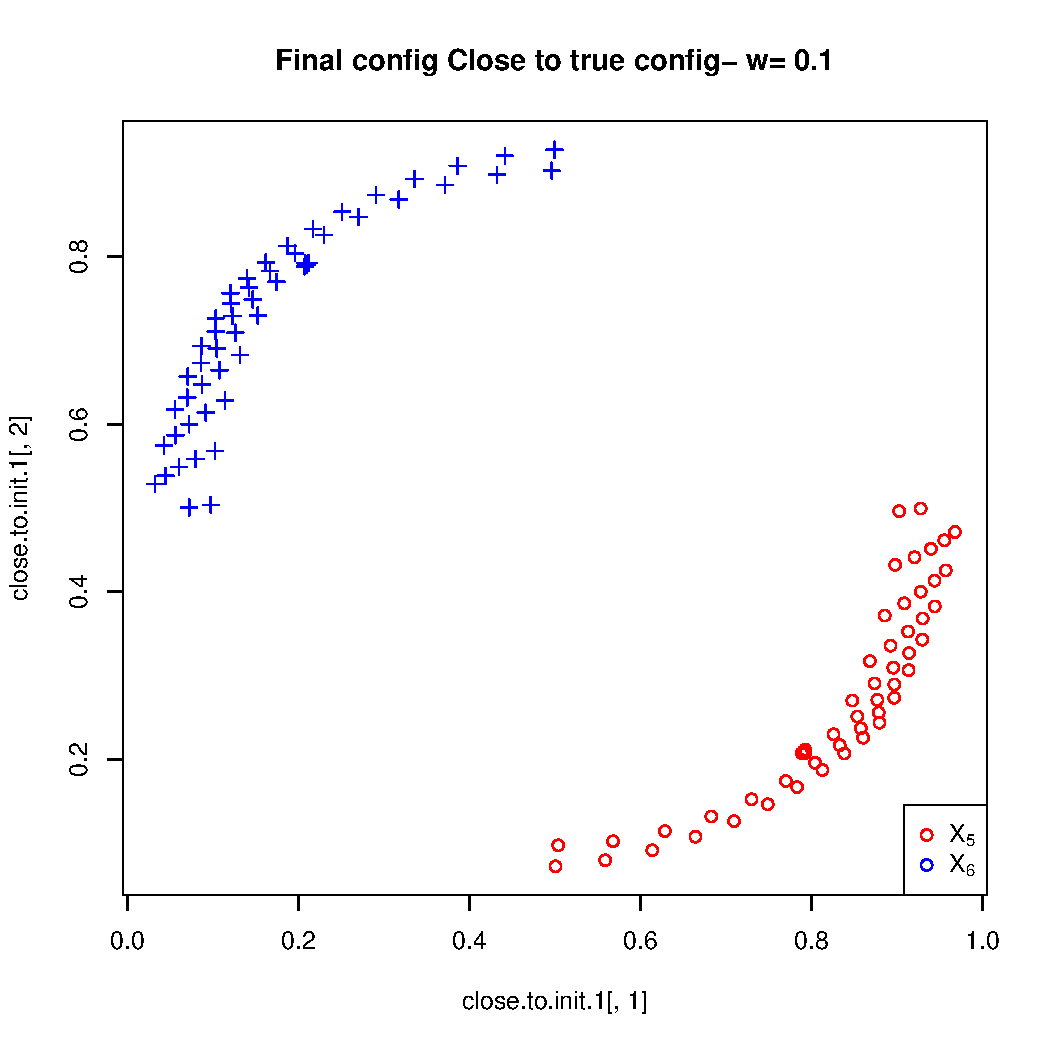
\includegraphics[scale=0.45]{true-min-w-0_1.pdf}

\label{fig:Finalconfig-MultMin-w-0_1_a}
\end{minipage}
\hspace{0.5cm}
\begin{minipage}[b]{0.5\linewidth}
\centering
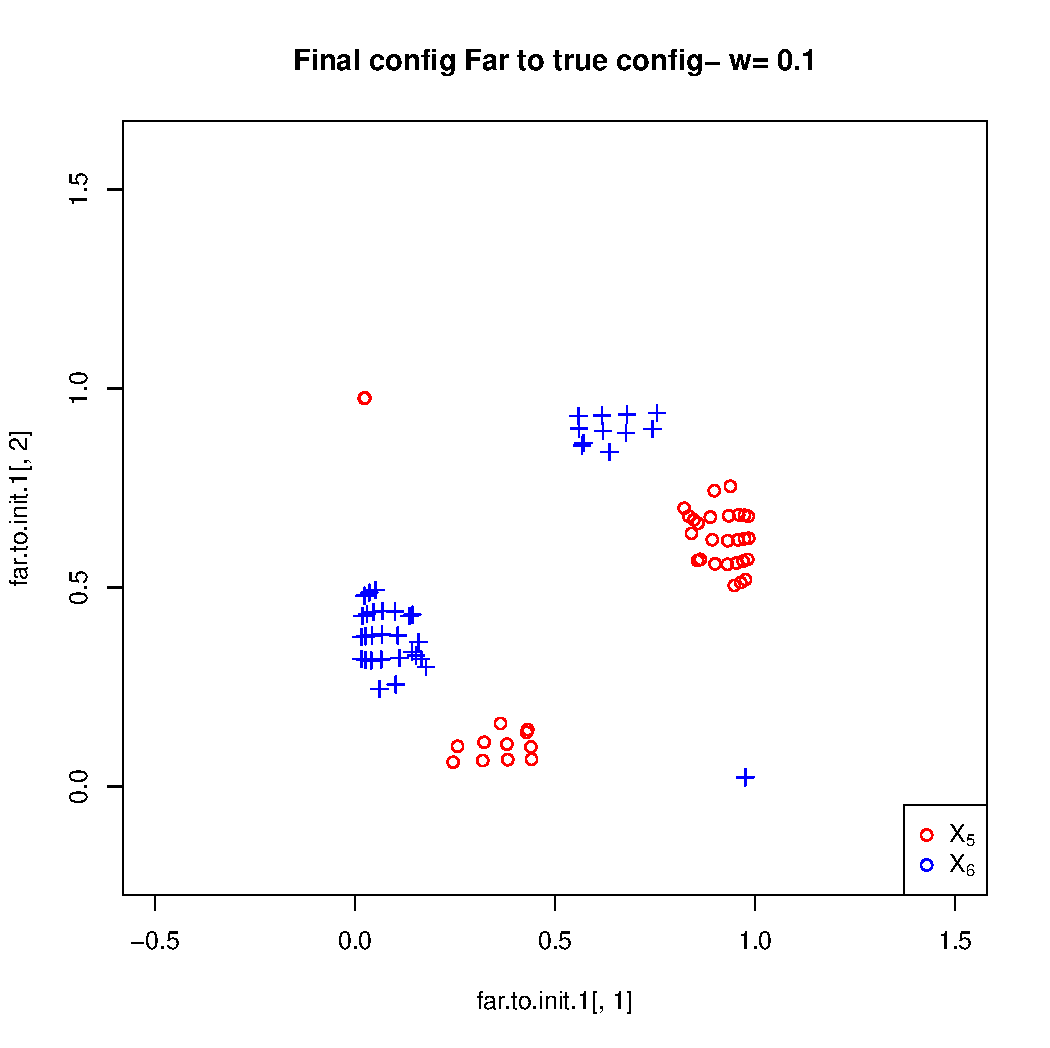
\includegraphics[scale=0.45]{other-min-w-0_1.pdf}

\label{fig:Finalconfig-MultMin-w-0_1_b}
\end{minipage}

\caption{Final configurations for for different $w=0.1$ }
\label{fig:Finalconfig-MultMin-w-0_1}


\end{figure}




\begin{figure}
\begin{minipage}[b]{0.5\linewidth}
\centering
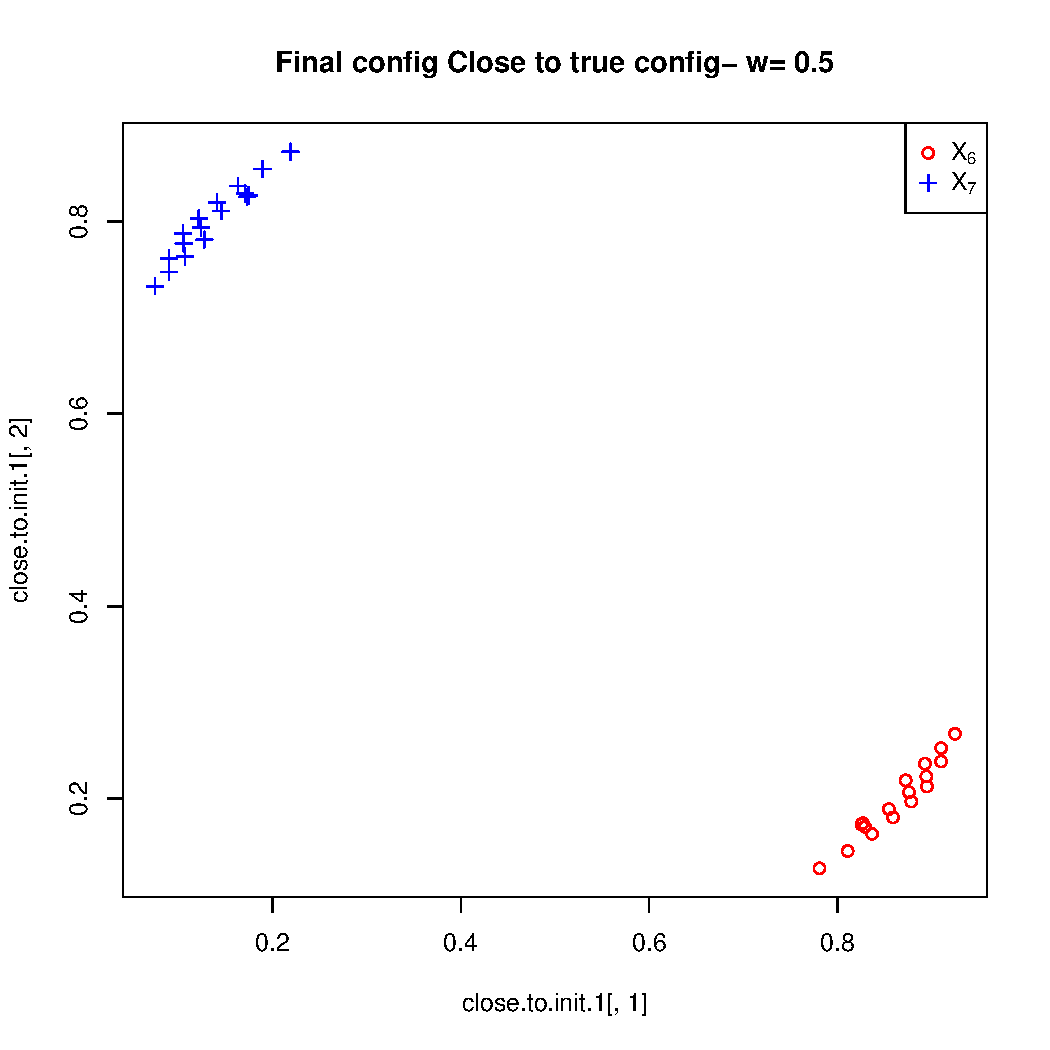
\includegraphics[scale=0.45]{true-min-w0_5}

\label{fig:Finalconfig-MultMin-w-0_5_a}

\end{minipage}
\hspace{0.5cm}
\begin{minipage}[b]{0.5\linewidth}
\centering
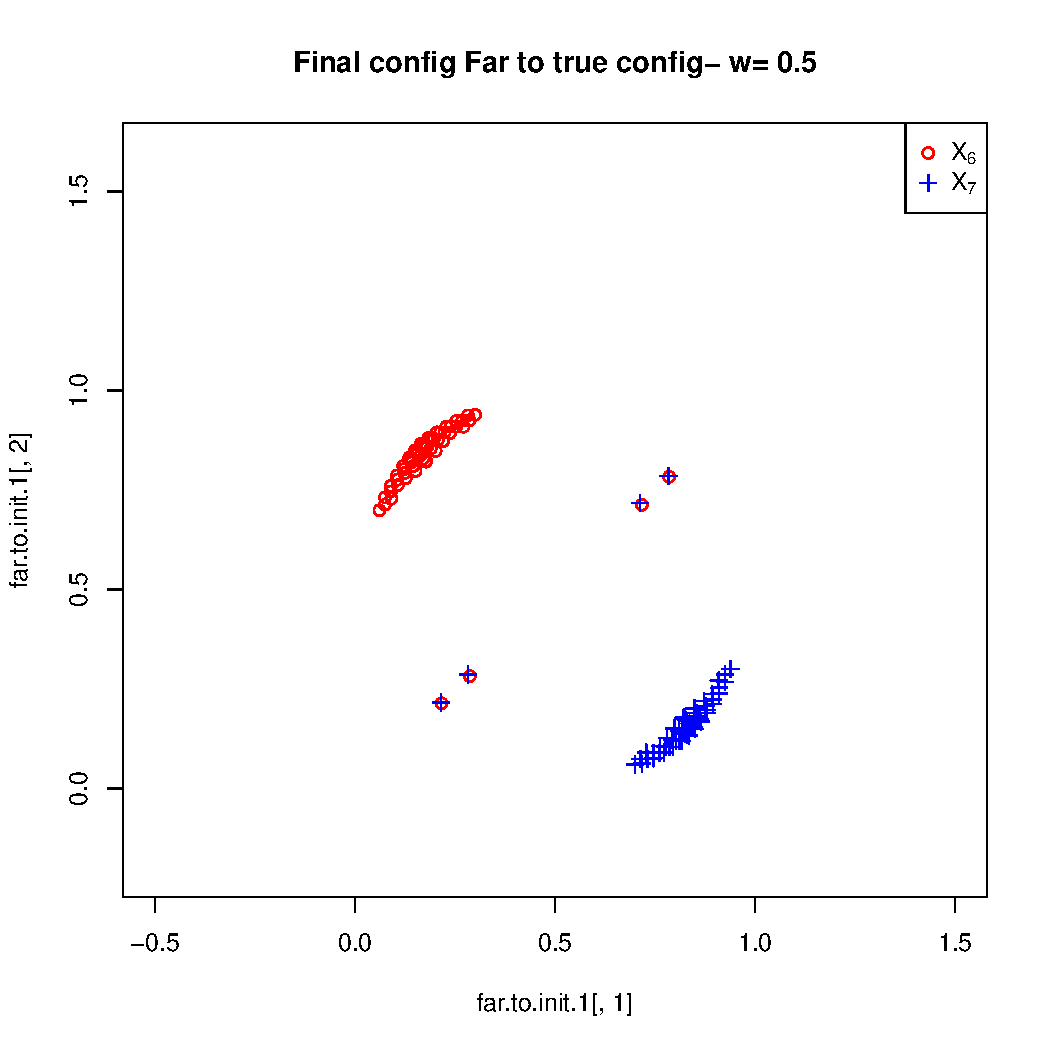
\includegraphics[scale=0.45]{other-min-w0_5.pdf}

\label{fig:Finalconfig-MultMin-w-0_5_b}

\end{minipage}

\caption{Final configurations for for different $w=0.5$ }
\label{fig:Finalconfig-MultMin-w-0_5}

\end{figure}

\begin{figure}
\begin{minipage}[b]{0.5\linewidth}
\centering
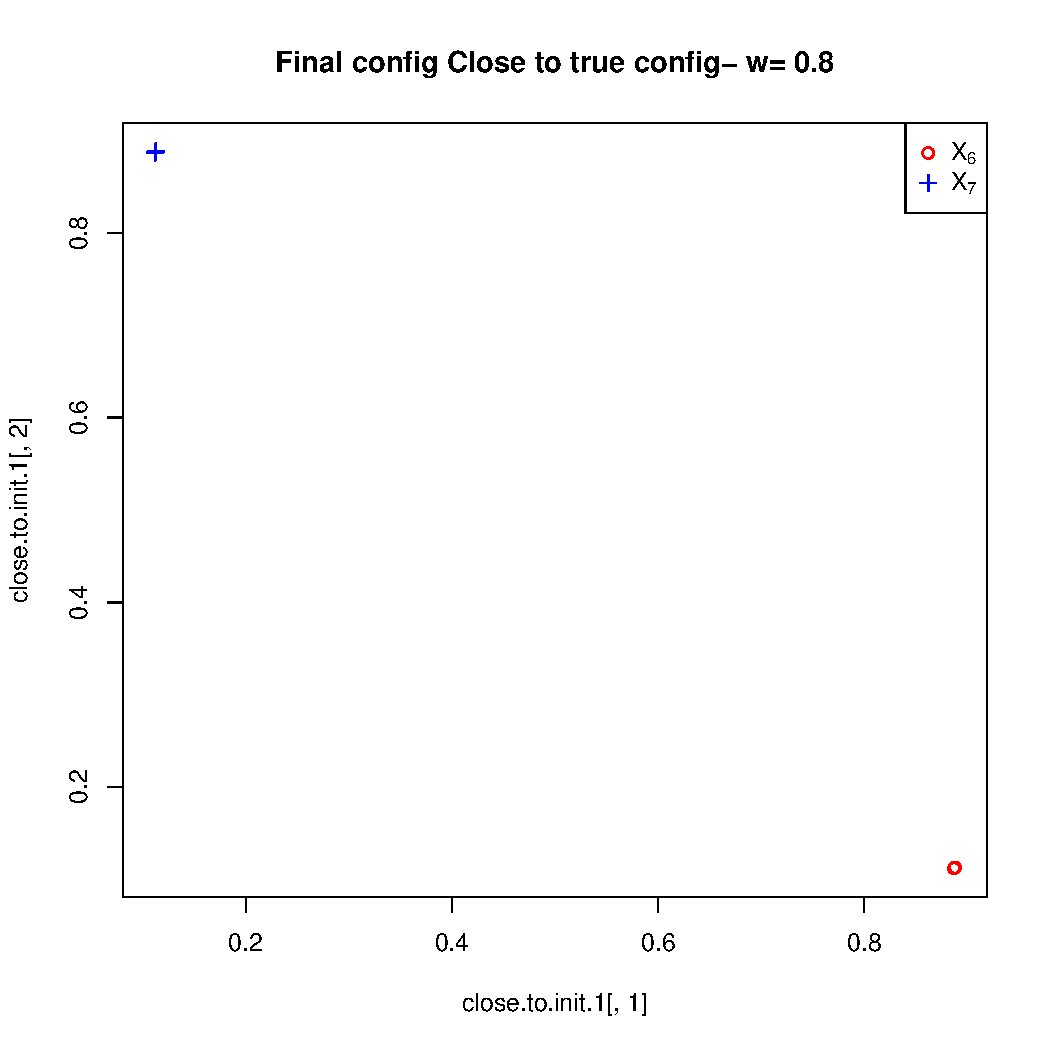
\includegraphics[scale=0.45]{true-min-w0_8.pdf}
\label{fig:Finalconfig-MultMin-w-0_8_a}


\end{minipage}
\hspace{0.5cm}
\begin{minipage}[b]{0.5\linewidth}
\centering
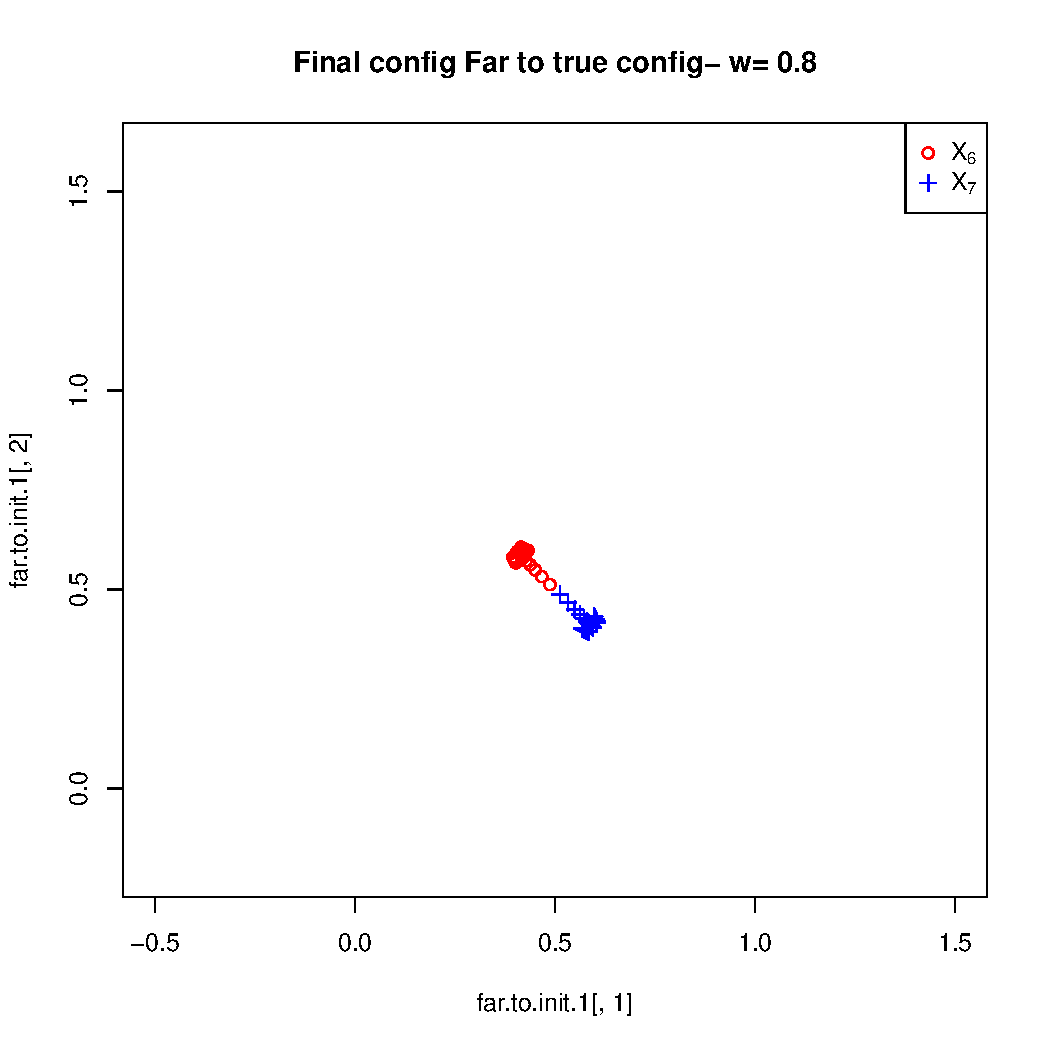
\includegraphics[scale=0.45]{other-min-w0_8.pdf}
\label{fig:Finalconfig-MultMin-w-0_8_a}


\end{minipage}

\caption{Final configurations for for different $w=0.8$ }
\label{fig:Finalconfig-MultMin-w-0_8}

\end{figure}



\begin{figure}
\begin{minipage}[b]{0.5\linewidth}
\centering
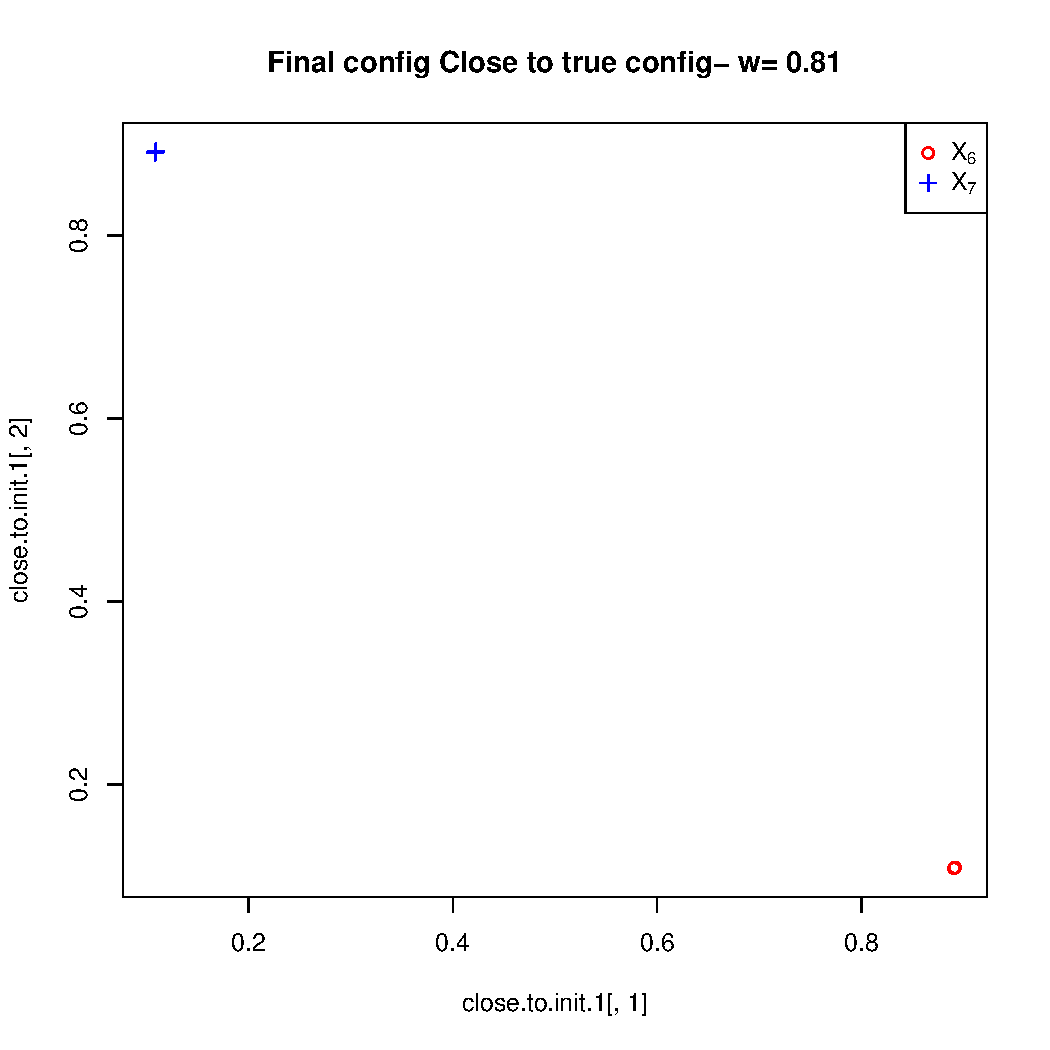
\includegraphics[scale=0.45]{true-min-w0_81.pdf}


\end{minipage}
\hspace{0.5cm}
\begin{minipage}[b]{0.5\linewidth}
\centering
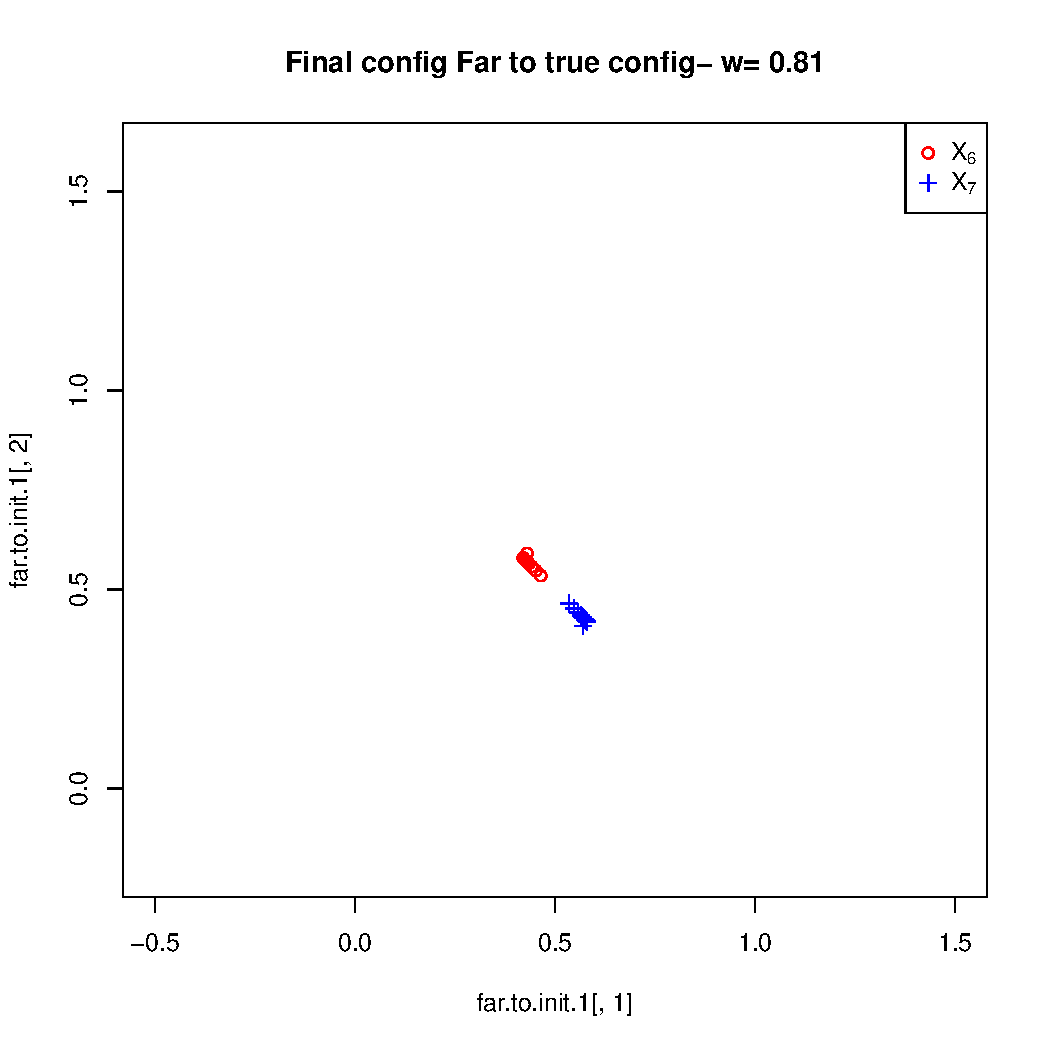
\includegraphics[scale=0.45]{other-min-w0_81.pdf}


\end{minipage}

\caption{Final configurations for for different $w=0.81$ }
\label{fig:Finalconfig-MultMin-w-0_81}

\end{figure}




\begin{figure}
\begin{minipage}[b]{0.5\linewidth}
\centering
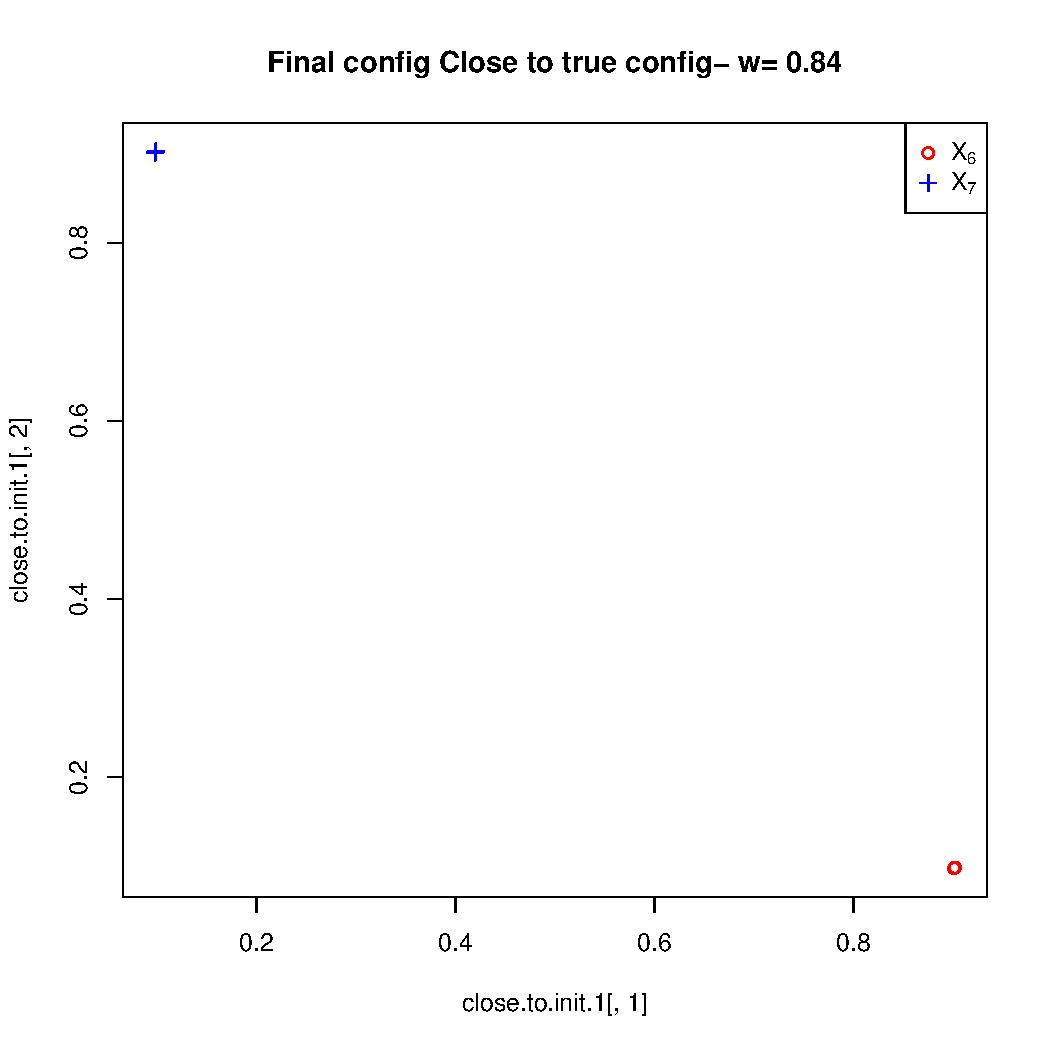
\includegraphics[scale=0.45]{true-min-w0_84.pdf}

\label{fig:figure2-1}
\end{minipage}
\hspace{0.5cm}
\begin{minipage}[b]{0.5\linewidth}
\centering
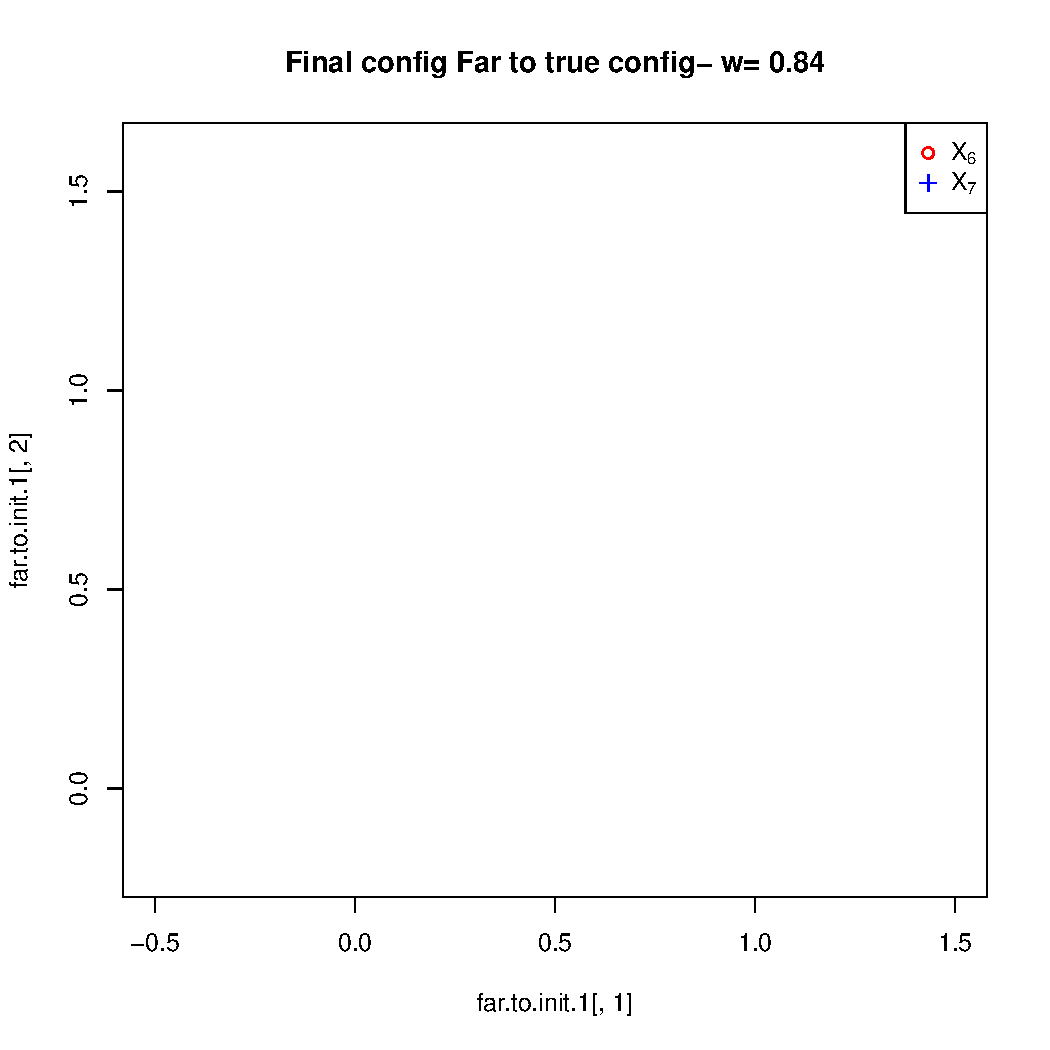
\includegraphics[scale=0.45]{other-min-w0_84.pdf}


\end{minipage}

\caption{Final configurations for for different $w=0.84$ }
\label{fig:Finalconfig-MultMin-w-0_84}

\end{figure}



% latex table generated in R 2.15.1 by xtable 1.7-0 package
% Sat Jan 05 00:54:38 2013

\begin{landscape}
\begin{table}[ht]
\def\h#1{\multicolumn{1}{p{3em}}{\mbox{}\hskip0pt #1}}
\begin{center}

\begin{tabular}{r|rrrrrrrrrrrrrrrrrrrrrrrrrrrrrrrrrrrr}
\hline
$w$ & 0.1 & 0.2 & 0.3 & 0.4 & 0.41 & 0.42 & 0.43 & 0.44 & 0.45 & 0.46 & 0.47  \\ 
\hline
Local min for real config. & 2.80 & 2.51 & 2.22 & 1.92 & 1.89 & 1.86 & 1.83 & 1.80 & 1.77 & 1.74 & 1.71 \\ 
Alternative local min & 0.39 & 0.76 & 1.10 & 1.40 & 1.43 & 1.46 & 1.48 & 1.51 & 1.53 & 1.56 & 1.58 \\ 
\hline
\end{tabular}


\begin{tabular}{r|rrrrrrrrrrrrrrrrrrrrrrrrrrrrrrrrrrrr}
\hline
$w$ & 0.48 & 0.49 & 0.5 & 0.51 & 0.52 & 0.53 & 0.54 & 0.55 & 0.6 & 0.65 & 0.7 \\ 
\hline
Local min for real config. &  1.68 & 1.65 & 1.62 & 1.59 & 1.56 & 1.53 & 1.50 & 1.47 & 1.32 & 1.17 & 1.01   \\ 
Alternative local min &  1.60 & 1.63 & 1.65 & 1.67 & 1.69 & 1.71 & 1.73 & 1.74 & 1.81 & 1.82 & 1.81  \\ 
\hline
\end{tabular}



\begin{tabular}{r|rrrrrrrrrrrrrrrrrrrrrrrrrrrrrrrrrrrr}
\hline
$w$ & 0.75 & 0.76 & 0.77 & 0.78 & 0.79 & 0.8 & 0.81 & 0.82 & 0.83 & 0.84 & 0.85  \\ 
\hline
Local min for real config. &  0.86 & 0.82 & 0.79 & 0.76 & 0.73 & 0.70 & 0.66 & 0.63 & 0.60 & 0.57 & 0.53  \\ 
Alternative local min &   1.79 & 1.77 & 1.75 & 1.72 & 1.69 & 1.66 & 1.64 & NA & NA & NA & NA \\ 
\hline
\end{tabular}

\end{center}

\caption{Final stress values for the two local minima configurations\label{table:stress_val}}
\end{table}

\end{landscape}





\begin{comment}
%old results

\begin{table}[ht]
\begin{center}
\begin{tabular}{rrrrrr}
\hline
$w$ value & 0.1 & 0.45 & 0.5 & 0.55 & 0.99 \\ 
\hline
Local min for real config. & 2.80 & 1.77 & 1.62 & 1.47 & 0.04 \\ 
Alternative local min & 0.39 & 1.53 & 1.65 & 1.74 & NA \\ 
\hline
\end{tabular}
\end{center}
\label{table:stress_val}
\end{table}
\end{comment}

\begin{knitrout}
\definecolor{shadecolor}{rgb}{0.969, 0.969, 0.969}\color{fgcolor}\begin{kframe}


{\ttfamily\noindent\bfseries\color{errorcolor}{\#\# Error: could not find function "{}ggplot"{}}}

{\ttfamily\noindent\bfseries\color{errorcolor}{\#\# Error: object 'g2' not found}}\end{kframe}
\end{knitrout}



This example was constructed carefully with a symmetric configuration of points. Under reasonable probability distributions for point configurations, it is unexpected that such a symmetry will appear with non-zero probability. Thus, we conjecture that such discontinuities with respect to $w$ in the embedded configuration  have zero measure. Since the test statistic is a continuous function of the embedded configuration, this would mean that the event that the test statistic has discontinuities with respect to $w$ also have zero measure. This suggests the assumption of stochastic continuity of the test statistic  that is used to show the continuity of $AUC$ function in \autoref{subsec:auc_cont} is a reasonable assumption.

%Other than such carefully constructed examples, it is  unexpected that slight changes in $w$  will change the ordering of the ``distinct''  local minima according to their stress values.
%Therefore,  the argmin among the local minima configurations is independent of $w$. The minimum configuration is then a continuous function of $w$. 
%By the continuity of the distance function with respect to configurations, the test statistic is continuous with respect to $w$. One can conclude  that stochastic continuity  is a valid assumption and $\beta(w) $ is a continuous function of $w$. 
%It is possible this is not the global minimum in $\mathbb{R}^d$  

%Does the discontinuity in configurations mean discontinuity  in the $\beta(w)$ function
%It is possible this is not the global minimum in $\mathbb{R}^d$  

%\section[Optional table of contents heading]{Dependence of globality of local minima on $w$}




\chapter{Simulations and Experiments}
\label{sec:simexp_results}
\chaptermark{Simulations and Experiments}





%Let us first investigate the effect of parameters on the empirical distribution of the test statistic, under null and alternative.
% For our Multivariate Normal and Dirichlet models, consider the signal and noise dimensions $p$ and $q$ respectively.
%  An increase in $p$ leads to the inflation of the test statistic under alternative
%  \ref{fig-stats-p}.


\section{Simulation Results\label{sec:Simulation Results}}
To compare the  different approaches, training data of matched pairs of measurements were generated according to the Dirichlet and Gaussian settings  with parameters $p,q,r,c$ \ref{chap:data_models}. Dissimilarity representations (\ref{sec:dissim_repr}) were computed from pairwise Euclidean distances of these measurements. A set of matched pairs and unmatched pairs of measurements were also generated for testing with the same distributions. Following the out-of-sample embedding of the dissimilarities test pairs (computed via by one of  P$\circ $M \ref{chap:PoM}, CCA \ref{chap:CCA}, regularized CCA \ref{sec:CCA} and JOFC \ref{chap:match_detection} approaches),  test statistics  for matched and unmatched pairs (corresponding to null and alternative hypothesis, respectively) were used to compute power values at a set of fixed type I error rate $\alpha$ values. By using the same generated data for all of the approaches, we are able to compare the performance of  different approaches either using the area under curve (AUC) measure or the statistical power at a desired $\alpha$ value.

 Additionally, to consider  relative robustness of methods , ``noisy" measurements were created from the original measurements by concatenating randomly generated independent noise vectors (\autoref{subsec:noise}).   This setting will be referred to as the ``noisy case". The magnitude of noise is controlled by the parameter $c$ in equation \eqref{eq:noise-expr}). The original setting, with $c=0$,  will be referred as the ``noiseless case".
If the magnitude of noise is small enough, and the embedding dimension is not larger than signal dimension, the embeddings provided by PCA and MDS should not be affected significantly by the noise. However  if the number of noise dimensions (controlled by the parameter $q$ in the distribution of $E_{ik}$ as defined in equation \eqref{eq:noise-expr} ) is large enough, it is expected that embeddings via  CCA  will  be affected due to spurious correlation between noisy dimensions.

We will now describe the steps for our Monte Carlo simulation in detail. Given the setting ("Gaussian","Dirichlet"),   the steps for each Monte Carlo replicate are as follows:
\begin{itemize}
\item A training set ($\mathbf{T}_{mc}$) which consists of  $n$ pairs of matched measurements is generated.  If $c=0$, the ``noiseless" data setting is being simulated and measurements are $p$-dimensional vectors, otherwise  the ``noisy" setting is being used to generate data and measurement vectors are $(p+q)$-dimensional. $ \mathbf{T}_{mc}$ = 
$\begin{array}{ccc}
        X_{11} & \ldots & X_{1K} \\
        \cdots & \cdots      & \cdots   \\ 
        X_{n1} & \ldots     & X_{nK} \\
    \end{array}
$
 where each $X_{ik}$ is a random vector of dimension $(p+q \times \I (c>0))$ and the conditional distribution  $X_{i.}|\bm{\alpha}_i  $ is specified as an appropriate Multivariate Normal or Dirichlet distribution. The data generation is also described in detail \autoref{chap:data_models}
\item  Dissimilarities are computed from $X_{ik}$, $\left[\Delta_{k}\right]_{ij}=d(X_{ik},X_{jk})$ for each condition $k$. We use Euclidean Distance for both Gaussian and Dirichlet settings.
\item Dissimilarities are embedded in  Euclidean space  via MDS. For P$\circ$M approach, the embedding is into $\R^d$ followed by a transformation from  $\R^d$ to  $\R^d$. For CCA , the embedding is into $\R^{p+q}$ , followed by projection into $\R^d$. For regularized CCA,  the embedding is into $\R^{s}$ where $s=(p+q)/2$\footnote{$s$ could be chosen as any integer between $d$ and $p+q$. This particular choice was a sensible one for the values of $p,q,d$ in our simulations.} , followed by projection into $\R^d$. The final embeddings lie in $\R^d$.   Denote this in-sample embedding configuration as   $\hat{\mathbf{T}}$. For JOFC approach, embedding is carried out with the weighted raw stress function $\sigma_{W}(\cdot)=f_{w}(D(\cdot),M)$ in equation \eqref{fid-comm-tradeoff-func} with a common weight $w$ for commensurability terms and another common weight $1-w$ for fidelity terms. We try different values of $w$ in our simulations. For P$\circ$M, CCA and regularized CCA, unweighted raw stress function ($\sigma(\cdot)$) is used as a criterion function for embedding the dissimilarities.
%These are \emph{non-uniform} and \emph{uniform}  weighting, respectively.

\item  $m$ pairs of matched   measurements are generated which are treated as out-of-sample, and 
\begin{itemize}
\item compute the dissimilarities  %$\mathbf{\Delta}^{new}={ \delta_{ik}^{new}; i=1,\ldots, n;\hspace{5pt} k=1,2}$
 between these out-of-sample  points and the points in ${\mathbf{T}_{mc}}$,  
\item  embed the OOS dissimilarities as pairs of embedded points via the OOS extension:\\
 $(\tilde{y}_1^{(1)},\tilde{y}_1^{(2)}),\ldots, (\tilde{y}_m^{(1)},\tilde{y}_m^{(2)})$, 
\item compute the test statistic $\tau$ for each pair, $\tau_i=d(\tilde{y}_i^{(1)},\tilde{y}_i^{(2)});\hspace{4pt}
i=1,\ldots,m$
\end{itemize}
 The values of the statistic $\tau={tau_i,i=1,\ldots,m}$ are used for computing  the empirical cumulative distribution function under null hypothesis. 

\item Identical steps for $m$ pairs of unmatched measurements result in the empirical cumulative distribution  function of $\tau$ under alternative hypothesis.
\item For any fixed $\alpha$ value, a critical value for the test statistic and the corresponding power is computed.
\end{itemize}



\begin{figure}
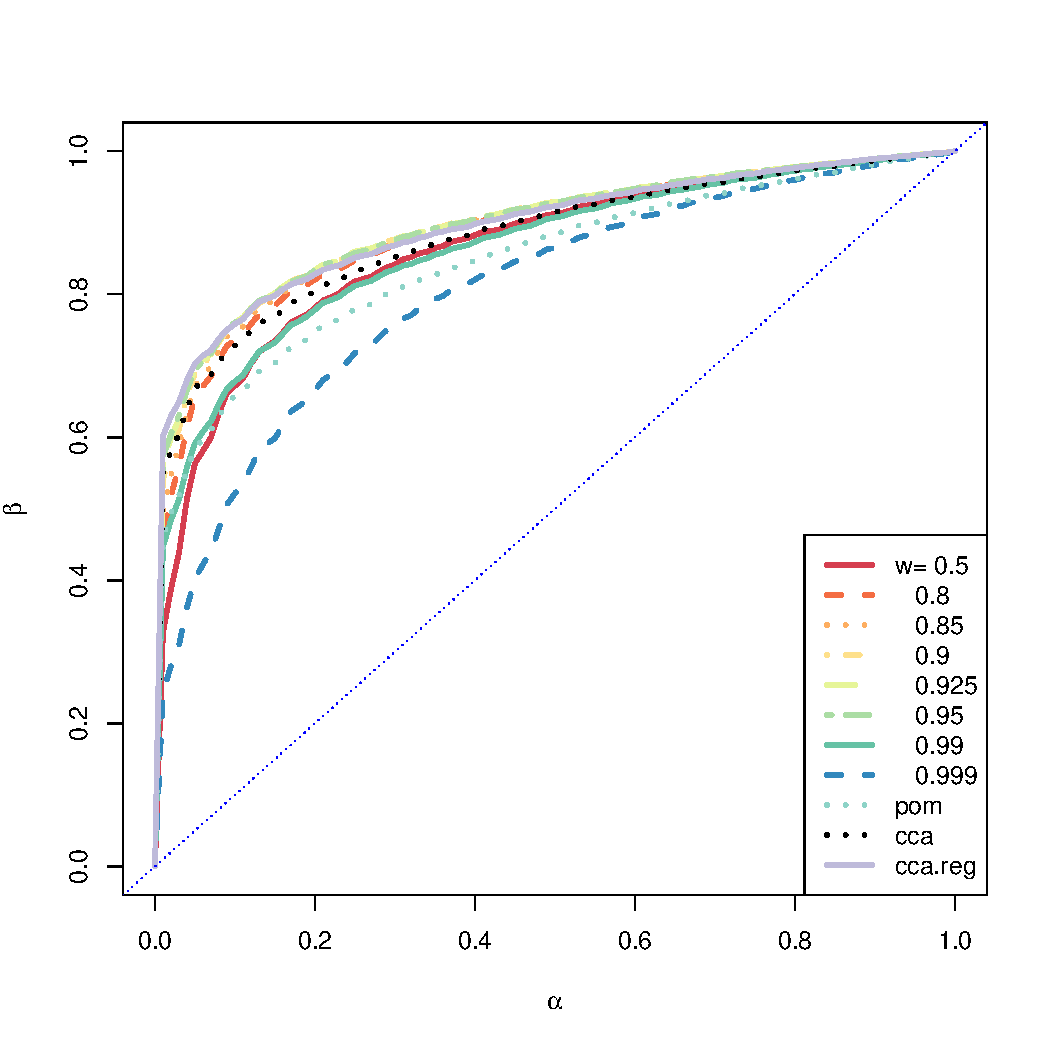
\includegraphics[scale=0.75]{MVN-FC-Tradeoff-OOS-c0_01.pdf}
\caption{Power ($\beta$) vs Type I error ($\alpha$) plot for different $w$ values for the Gaussian setting (noisy case)}
\label{fig:MVN-c001-power-alpha}
\end{figure}

\begin{figure}
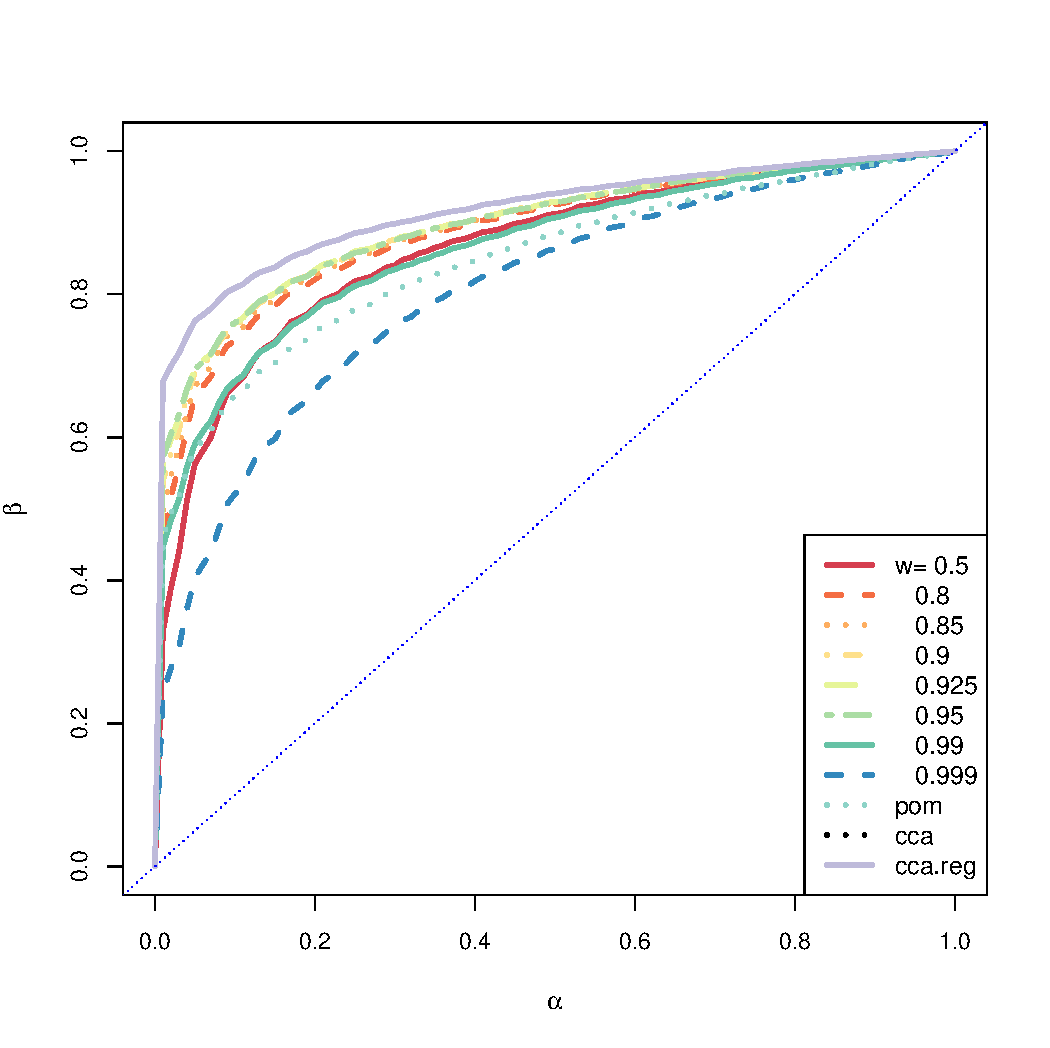
\includegraphics[scale=0.75]{MVN-FC-Tradeoff-OOS-c0.pdf}
\caption{Power ($\beta$) vs Type I error ($\alpha$) plot for different $w$ values for the Gaussian setting (noiseless case)}
\label{fig:MVN-c0-power-alpha}
\end{figure}

\begin{figure}
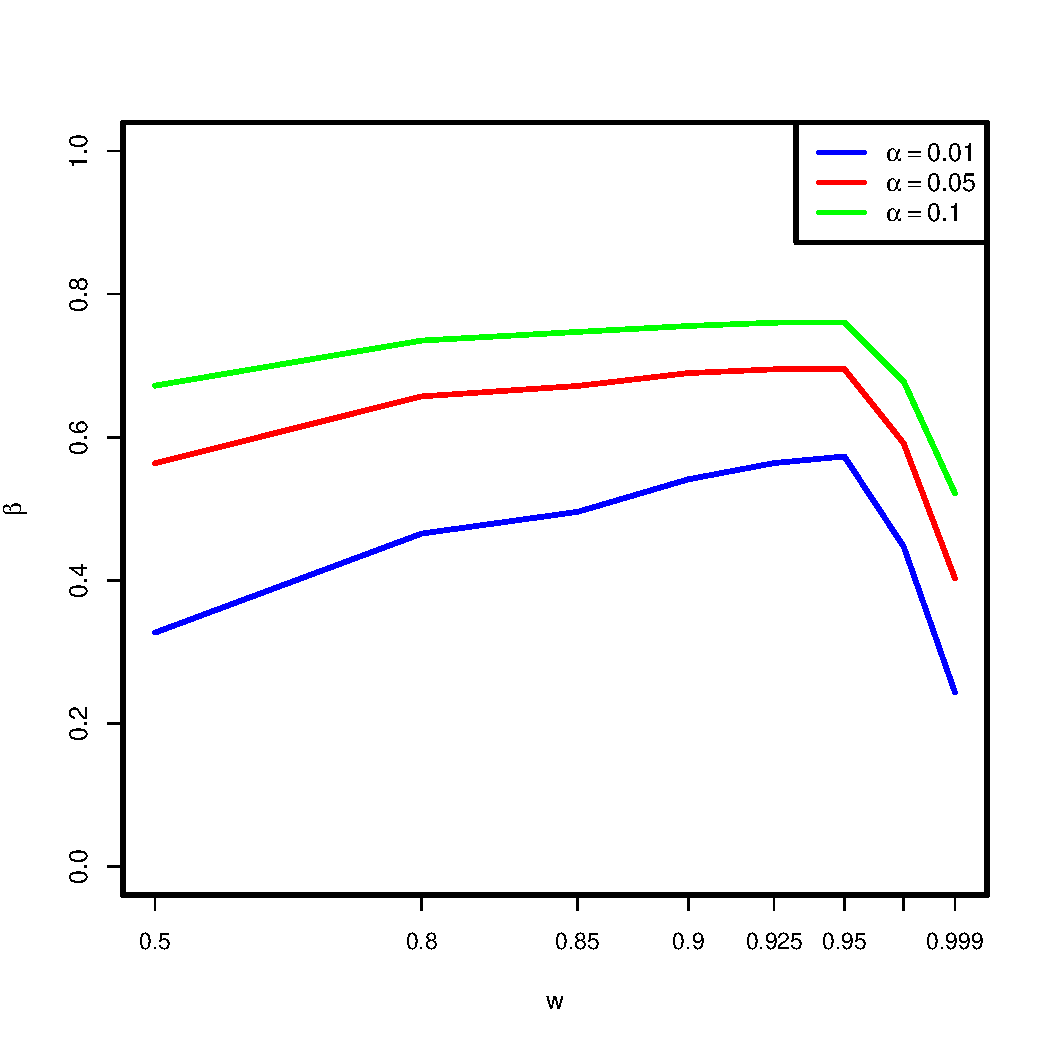
\includegraphics[scale=0.75]{OOSMVN-power-w-c0_01.pdf}
\caption{Power ($\beta$) vs $w$ plot for different Type I error ($\alpha$) values for the Gaussian setting (noisy case)}
\label{fig:MVN-c001-power-w}
\end{figure}


\begin{figure}
\includegraphics[scale=0.75]{Dirichlet-FC-Tradeoff-OOSc0-01-n150.pdf}
\caption{Power ($\beta$) vs Type I error ($\alpha$) plot for different $w$ values for the Dirichlet setting (noisy case)}
\label{fig:Dir-c001-power-alpha}
\end{figure}

\begin{figure}
\includegraphics[scale=0.75]{Dirichlet-FC-Tradeoff-OOSc0-n150.pdf}
\caption{Power ($\beta$) vs Type I error ($\alpha$) plot for different $w$ values for the Dirichlet setting (noiseless case)}
\label{fig:Dir-c0-power-alpha}
\end{figure}

\begin{figure}
\includegraphics[scale=0.80]{OOSDirichlet-power-w-c0-01.pdf}
\caption{Power ($\beta$) vs $w$ plot for different Type I error ($\alpha$) values for the Gaussian setting (noisy case)}
\label{fig:Dir-c001-power-w}
\end{figure}

For $p=5$,$q=10$,$d=2$, and $c\in{0,0.01}$, for $n=150$ and $m=150$, the average of the power values for $nmc=150$ Monte Carlo replicates are computed at  different $\alpha$s and are plotted in Figure \ref{fig:MVN-c001-power-w} against $\alpha$ for the Gaussian setting.  
%Qualititatively similar plots for the Dirichlet setting  are not included for brevity.  
The plot in \autoref{fig:MVN-c001-power-w} shows that for different values of  $w$, $\beta$-$\alpha$ curves vary significantly.  The conclusion is that the match detection tests with JOFC embedding using specific $w$ values have better performance than other $w$ values in terms of power.  In Figure
 \ref{fig:MVN-c001-power-w},  $\beta(w)$ is plotted against $w$ for fixed values of $\alpha$. It is  interesting that the optimal value of $w$ seems to be in the range of $(0.85,1)$ for all settings, which suggests a significant emphasis on commensurability might be  critical for the match detection  task. 




\begin{comment}
\begin{figure}
\includegraphics[scale=0.75]{OOS-MVN-power-w-c0.pdf}
\caption{$\beta$ vs $w$ plot for fixed $\alpha$ values for the Gaussian setting (noiseless case)}
\label{fig:MVN-c0-beta-w}
\end{figure}


\begin{figure}
\includegraphics[scale=0.65]{OOSMVN-power-w-c001.pdf}
\caption{Power ($\beta$) vs $w$ plot for fixed Type I error ($\alpha$) values for the Gaussian setting (noisy case)}
\label{fig:MVN-c001-beta-w}
\end{figure}

\end{comment}

Note that in Figure \ref{fig:MVN-c001-power-w} for $\alpha=0.05$, $\beta_{\alpha=0.05}(w=0.99)\geq\beta_{\alpha=0.05}(w=0.5)$. However, for $\alpha=0.3$, $\beta_{\alpha=0.3}(w=0.99)\leq\beta_{\alpha=0.3}(w=0.5)$. This justifies our comment that  $w^{*}$  must be defined with respect to  the AUC measure or a specific $\alpha$ value.


\begin{comment}
\begin{figure}
\includegraphics[scale=0.75]{OOS-Dirichlet-power-w-c0.pdf}
\caption{$\beta$ vs $w$ plot for fixed $\alpha$ values for the Dirichlet setting(noiseless case)}
\label{fig:fig7}
\end{figure}

\begin{figure}
\includegraphics[scale=0.35]{OOS-Dirichlet-power-w-c0-01.pdf}
\caption{$\beta$ vs $w$ plot for fixed $\alpha$ values for the Dirichlet setting(noisy case)}
\label{fig:fig8}
\end{figure}
\end{comment}



Note that  for all of the settings, the estimate of the optimal $w^{*}$ has  higher power than $w$=0.5 (the unweighted case).
To test the statistical significance of this observation, we consider the following hypothesis test:  the null hypothesis that  $\mcH_{0}: \beta_{\alpha}({\hat{w}^*})\leq\beta_{\alpha}({w=0.5})$  is tested against the alternative $\mcH_{A}=\beta_{\alpha}({\hat{w}^*})>\beta_{\alpha}({w=0.5})$.  The least favorable null hypothesis is that  $\mcH_{0}: \beta_{\alpha}({\hat{w}^*})=\beta_{\alpha}({w=0.5})$.


McNemar's test will be used to compare the two predictors (referred to as $C_1$ and $C_2$ with $w$=0.5 and $w$=$w^*$ at a fixed $\alpha$ value.
\subsection{McNemar's Test\label{subsec:McNemarstest}}
Using previous notation,  the test statistic will be denoted by $T_a(w)$ under the alternative hypothesis and $T_0(w)$ under the null hypothesis.
For a fixed $\alpha$ value, one can compute two critical values $c(0.5)=max_l \{  P(T_0(0.5)>c)<\alpha\}$,  $c(w^*)=max_l \{  P(T_0(w_2)>c)<\alpha\}$. These critical values determine two binary classifiers, if we interpret the hypothesis testing as deciding whether a new pair is ``matched'' or not, and the test statistic as a score. Hypothesis testing is more nuanced than a binary decision problem, but for the sake of comparing two tests we can treat it as such.
%The values of the decision function that uses these critical  values, for each pair of embedded points (indexed by $i$, are  $(\tilde{y}_i^{(1)},\tilde{y}_i^{(2)}),\quad i=1,\ldots,m$.
To compare the  two statistical tests with  $w=0.5$ and $w$=$w^*$ , simulation result are used to compute $2\times 2$ contingency-tables of correct decisions and incorrect decisions made by each statistical test (or equivalently true and false classifications made by two classifiers). Let $\mathcal{D}$ denote the test dissimilarities for a new test pair, $\tau(\mathcal{D})$ the test statistic for the oos-embedding of that pair,$m_{\mathcal{D}}$ denote a binary variable whose value is $1$ if the pair is matched,$0$ otherwise. Denote decision outcome (whether the true or false decision is made) for the $i^{th}$ test pair by two binary variables $g_1^{i}$ and $g_2^{i}$,respectively.  If $g_1^{i} =1$ and $g_2^{i}=0$  for the $l^{th}$ MC replicate,  the first test made the correct decision and the second test made the incorrect decision with regard to the null and alternative hypotheses. 
\begin{align*}
g_1^{i}=\I(\I(\tau(\mathcal{D^{(i)}})>c(0.5))=m_{\mathcal{D}^{(i)}}) \textrm{for the first statistical test} \\
g_2^{i}=\I(\I(\tau(\mathcal{D^{(i)}})>c(w^*))=m_{\mathcal{D}^{(i)}}) \textrm{for the second statistical test}
\end{align*}
% McNemar's test was used to compare the two contingency tables for fixed $\alpha$. McNemar's test is a statistical test for %comparing two binary classifiers based on a 2-by-2 table of the counts of misclassifications of each. That is,
Consider the contingency table for the any Monte Carlo replicate given by $$G^{(l)}= \begin{array}{|c|c|}
      \hline
       e_{00}^{(l)} & e_{10}^{(l)}\\
      \hline
       e_{01}^{(l)} & e_{11}^{(l)}\\
      \hline
      \end{array}      $$  where  $e_{uv}^{(l)}=\sum_{i}{\I(\{g_1^{i}=u\} \&\& \{g_2^{i}=v\})}$ is equal to the number of instances at which the true hypothesis were identified  correctly ($g_1^{i}=1$) or incorrectly ($g_1^{i}=0$) by the first test, and correctly ($g_2^{i}=1$) or incorrectly ($g_2^{i}=0$) by the second test \emph{ in the $l^{th}$  MC replicate}.

Under the null  hypothesis that the two predictors have the same power at $\alpha$,
 $\Pry[\left(\{g_1^{i}=1\} \&\& \{g_2^{i}=0\}\right)]=\Pry[\left(\{g_1^{i}=0\} \&\& \{g_2^{i}=1\}\right)]$. Thus, a one-sided sign test is appropriate,  where the test statistic $e_{01}^{(l)}$ is distributed according to  the binomial distribution, $\mcB(e_{10}^{(l)}+e_{01}^{(l)},0.5)$. 

We consider simulated data with the noisy version of the Gaussian setting for this McNemar's test. The critical values $c(0.5)$ and $c(w^*)$ were computed for  allowable type I error $\alpha=0.05$ for the two tests. When comparing  the null hypothesis that  $\mcH_{0}: \beta_{\alpha}({\hat{w}^*})=\beta_{\alpha}({w=0.5})$ against the alternative $\mcH_{A}=\beta_{\alpha}({\hat{w}^*})>\beta_{\alpha}({w=0.5})$, the p-value is $p<1.09E-24$ which indicates the power using estimate of optimal $w^*$ is significantly greater than the power when using $w=0.5$.

Under the null distribution, we expect p-values for each MC replicate to be uniformly distributed. We find
 the distribution of p-values from McNemar's tests  is skewed and  we reject $\beta_{0.5}>=\beta_{w^*} $ for  55\%  of the Monte Carlo replicates.
%Insert plot here? 

\section{Effects of parameters of data model }
 Another avenue for investigation is  how the parameters of the distribution of  data such as $p$ ,$q$, $r$, $c$ and $d$ affect the results. We speculated  that as $q$, the number of   noise dimensions increases, the performance of  CCA approach would suffer, due to spurious correlations. We tested  our speculation using simulated data in the Gaussian Setting with $q=90$. The results are visualized in the  bundle of ROC curves in the Figure \ref{fig:largeq}.  Both CCA and  regularized CCA are not competitive with the JOFC approach with the appropriate $w$ values. In fact, the ROC curve for CCA is not very distinct from  random guess line. We conclude that CCA approach is not robust with respect to large number of noise dimensions, no matter what the magnitude  of the noise  is (which is controlled by the parameter $c$).

\begin{figure}
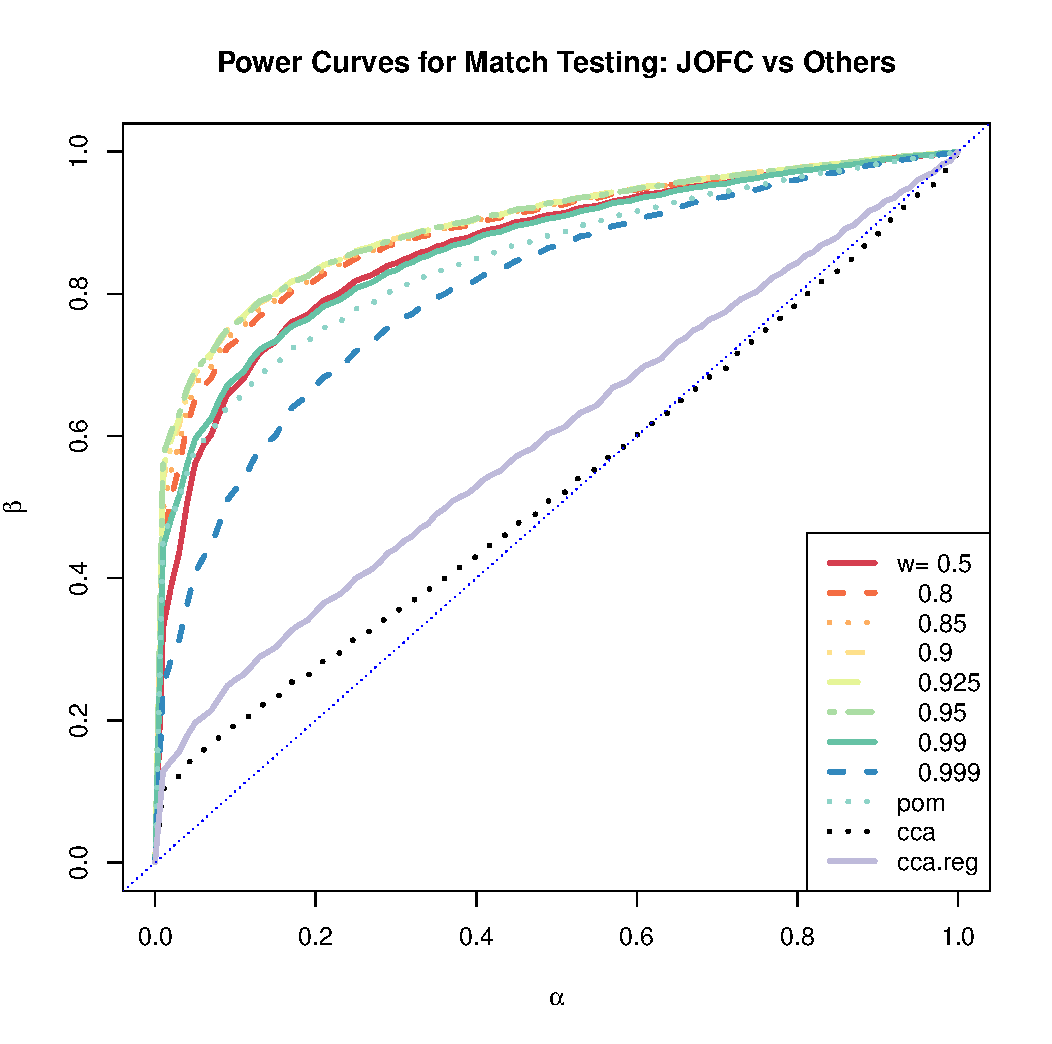
\includegraphics[scale=0.8]{MVN_JOFC_q_90_c_0_001}
\caption{Large Noise Dimension Behaviour of JOFC,P$\circ$ M and CCA approaches}
\label{fig:largeq}
\end{figure}


\section{Match Testing when the number of\\ conditions, $K$, is larger than 2\label{k_more_than_two_experiment}}


As it was mentioned, all of the approaches are generalizable to $K>2$ conditions, though an ambiguity need to be resolved. The alternative hypothesis could be  defined as the event that at least one of the K new dissimilarities are pairwise unmatched ($ H_{A1}: \exists i, j , 1\leq i < j \leq K :\bm{y}_{i} \nsim \bm{y}_{j} $ ) or it could be defined as the case that absolutely none of the K dissimilarities are pairwise matched   ($H_{A2}: \forall i, j , 1\leq i < j \leq K :\bm{y}_{i} \nsim \bm{y}_{j}$ ). We chose the alternative   $ H_{A1}$ for our simulations.
% and the sample from the alternative must be generated accordingly during Monte Carlo simulation. In the first case, an appropriate test statistic is then the maximum of the pairwise %distances between embeddings of each test K-tuple.

To adapt the P$\circ$M approach to this setting, one can use Procrustes analysis  generalized to more than two configurations. Generalized Procrustes Analysis \cite{GPCA} is described in \autoref{sec:GenProcrustes}.

We also have described generalized CCA in \autoref{sec:GenCCA}.  Of the different choices for the generalization of CCA, SUMCOR criterion was chosen.

To test whether P$\circ$M, JOFC, CCA and generalized CCA approaches are appropriate for this setting as well,
the simulations in \autoref{sec:Simulation Results} were repeated with $K$-condition data , generated by a multivariate normal model with $K=3$ conditions. 
 
 We investigate the  ``noisy" case for this setting , i.e. 
 $q$-dimensional noise vectors of magnitude $c$ were added to the matched measurements, and ``signal" vectors were multiplied by $1-c$.  
 
 The ROC curves for these simulations are shown in \ref{fig:MVN-c001-power-w-Kcond}.


\begin{figure}
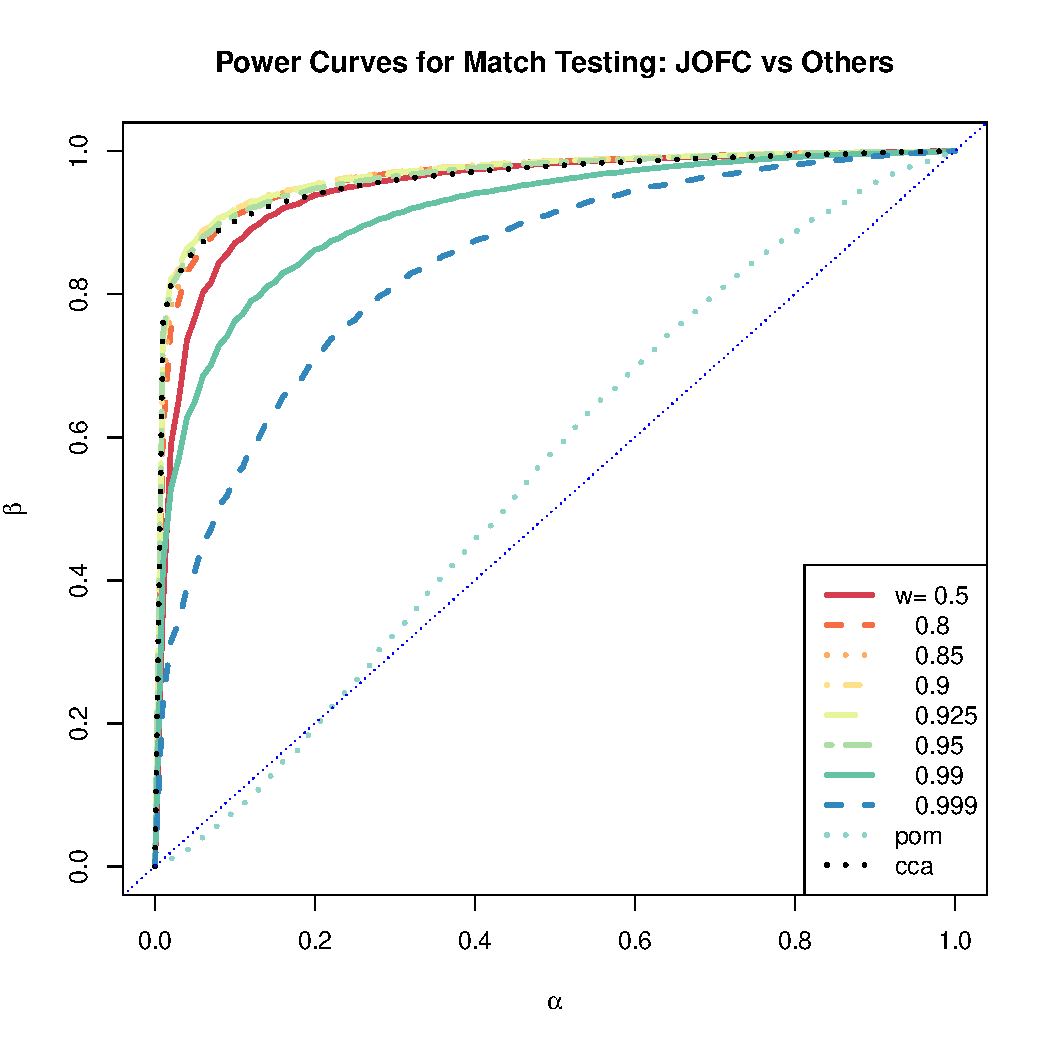
\includegraphics[scale=0.95]{MVN-FC-Tradeoff-OOS-3cond.pdf}
\caption{Power ($\beta$) vs Type I error ($\alpha$) plot for different $w$ values for the Gaussian setting with $K=3$ conditions (noisy case)}
\label{fig:MVN-c001-power-w-Kcond}
\end{figure}

The results indicate a similar behaviour as $K=2$ case. Different  values of $w$ has significantly different ROC curves. This shows that JOFC is a suitable approach for match detection using $K>2$ conditions as well as $K=2$ conditions.


\section{Experiments on Wiki Data}
To test the JOFC approach with real data, a collection of articles are collected from the English Wikipedia, consisting of the
 directed 2-neighborhood of the document "Algebraic Geometry". 
   This  collection of 1382 articles and the correspondence of each article in French 
Wikipedia is our real-life dataset. It is possible to utilize both textual content of the documents and the hyperlink graph structure. The textual content of the documents is summarized by the bag-of-words model. Dissimilarities between documents  in the same language are computed by the Lin-Pantel discounted mutual information \cite{LinPantel,PantelLin}
 and cosine dissimilarity $k(x_{ik}; x_{jk}) = 1 - (x_{ik} x_{jk})/(\|x_{ik}\|_2\|x_{ik}\|_2)$. 
 The dissimilarities based on the hyperlink graph of the collection of the articles are 
 for each pair of vertices $i$ and $j$, the number of vertices one must travel to go from $i$ to $j$.  Further details about this dataset is available in \cite{Zhiliang_disparate}.     
Only  dissimilarities based on the textual content will be considered for our experiments presented here.
   
The exploitation task is still testing for matchedness of vertices between different conditions, in this case wiki articles that are on the same topic  in  different languages.
For hypothesis testing,   randomly held out four documents - one matched pair and one unmatched pair
 -  are used to compute empirical type I error $\alpha$ and estimate of power based on the critical value computed
  from the distribution of the test statistic for the remaining 1380 matched pairs. 
The test statistic is computed using one of the three approached mentioned  CCA, P$\circ$M, and JOFC. 
The two sets of held-out matched pairs are embedded as $\tilde{y}_1$ and $\tilde{y}_2$, via out-of-sample
embedding, to estimate the null distribution of the test statistic $T_0 = d(\tilde{y}_1; \tilde{y}_2)$. This allows
us to estimate critical values for any specified Type I error level. 
Then the two sets of heldout unmatched pairs are embedded as $\tilde{y}_1^{(u)}$ and $\tilde{y}_2^{(u)}$, via out-of-sample embedding. 
$T_{a} = d(\tilde{y}_1^{(u)}; \tilde{y}_1^{(u)})$ will give us an empirical distribution of the test statistic  under the alternative hypothesis. 
And the distribution under null hypothesis and under alternative hypothesis can be used to estimate power.
Target dimensionality d is determined by the Zhu and Ghodsi  automatic dimensionality selection
method \cite{ZhuGhodsi}, resulting in d = 6 for this data set.


\begin{figure}
 \centering
\includegraphics[scale=0.8]{graphs/FidCommPaperwiki-two-cond-plot}
\caption{Match Detection using Wikipedia dataset. Different $w$ values listed in the legend correspond to different ROC curves.}
\end{figure}

The results show that a lot fidelity is prioritized more compared to Gaussian and Dirichlet simulations presented in \label{sec:Simulation Results}. Our conclusion is that there is no universal $w^*$, as its value depends on the data distribution and the inference task.


\section{Model Selection}
For the simulations presented up to now, the embedding dimension $d$ was set to 2. This was a convenient choice which allowed us to investigate various aspects of the JOFC and competing approaches.
However,  more care is required in selection of this parameter, since it plays such a big role in performance in general learning settings. To investigate the performance of JOFC approach as $d$ changes, we ran the usual Gaussian setting simulations. The signal dimension was set to $p=10$ and different $d=2,5,7,10,15$ values were used to test the JOFC approach.

The  plots of ROC curves in    \ref{fig:ROC-d} and  \ref{fig:ROC-d-15} shows the effect of $d$ parameter on the performance of different methods for the Gaussian setting for the noisy case.

\begin{figure}
 \centering
  \captionsetup[subfigure]{labelformat=empty}
        \begin{subfigure}[b]{0.5\textwidth}        
               \centerline{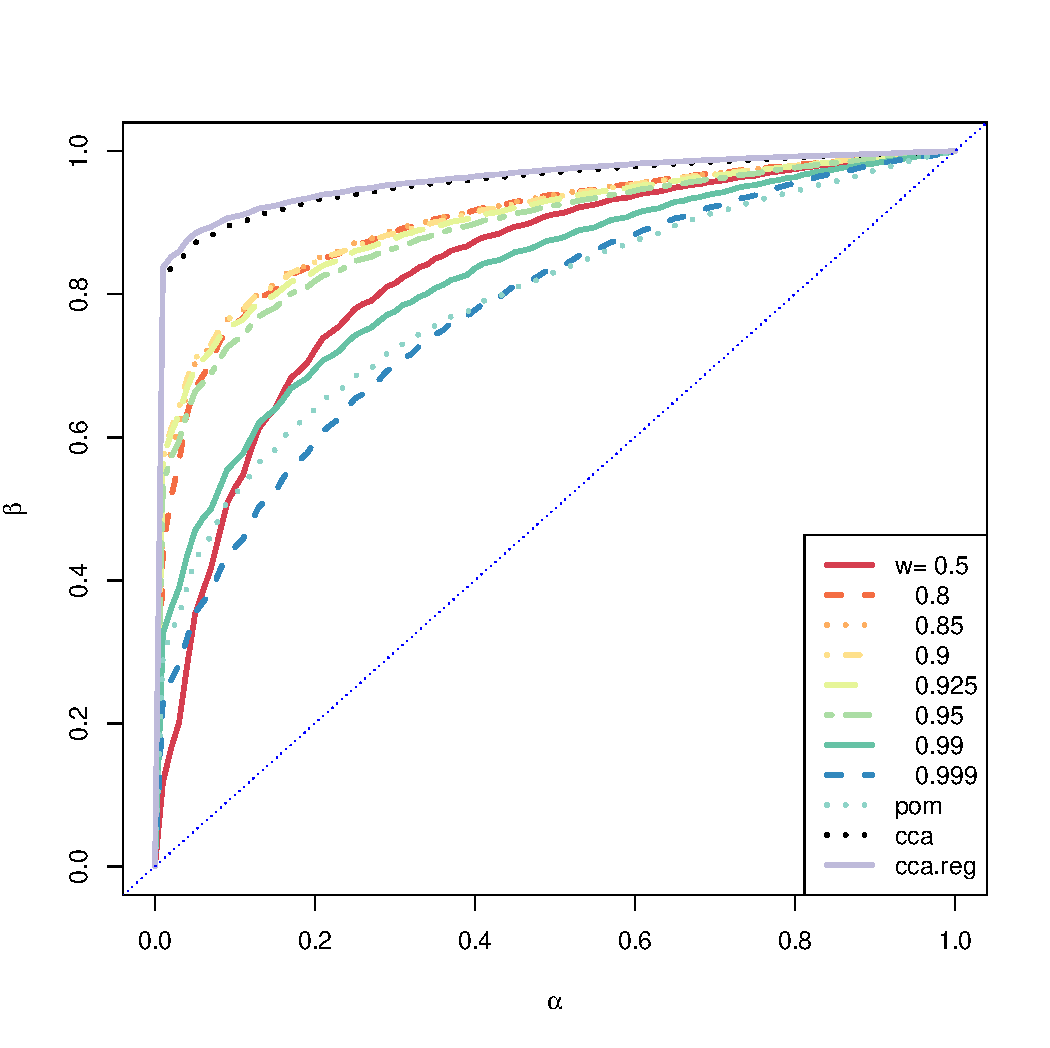
\includegraphics[width=\textwidth]{ROC-d-2.pdf}}
                \caption{d=2}
                \label{fig:ROC-d-2}
        \end{subfigure}%
         %add desired spacing between images, e. g. ~, \quad, \qquad etc. 
          %(or a blank line to force the subfigure onto a new line)
        \begin{subfigure}[b]{0.5\textwidth}           
                  \centerline{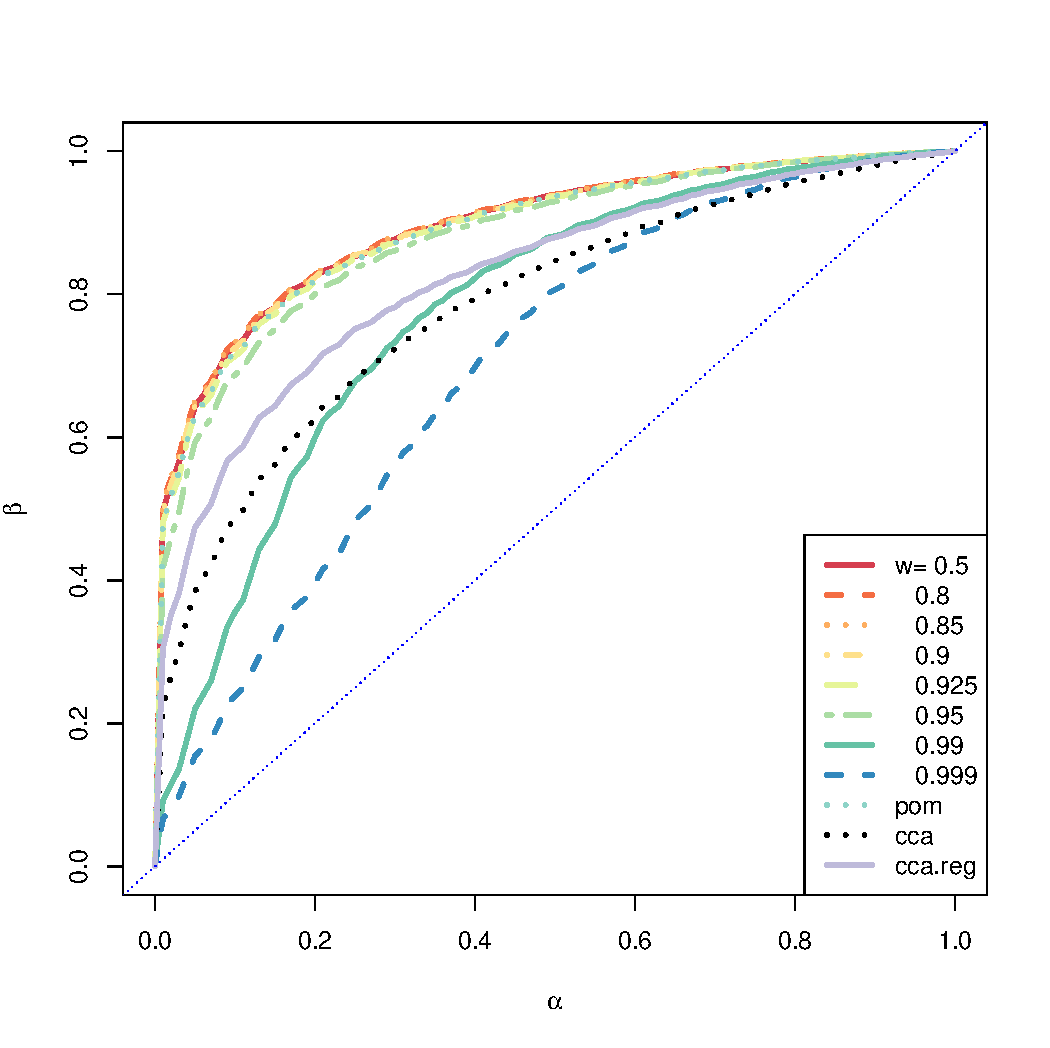
\includegraphics[width=\textwidth]{ROC-d-5.pdf}}
                \caption{d=5}
                \label{fig:ROC-d-5}
        \end{subfigure}      
        %add desired spacing between images, e. g. ~, \quad, \qquad etc.    %(or a blank line to force the subfigure onto a new line)
        \begin{subfigure}[b]{0.47\textwidth}             
               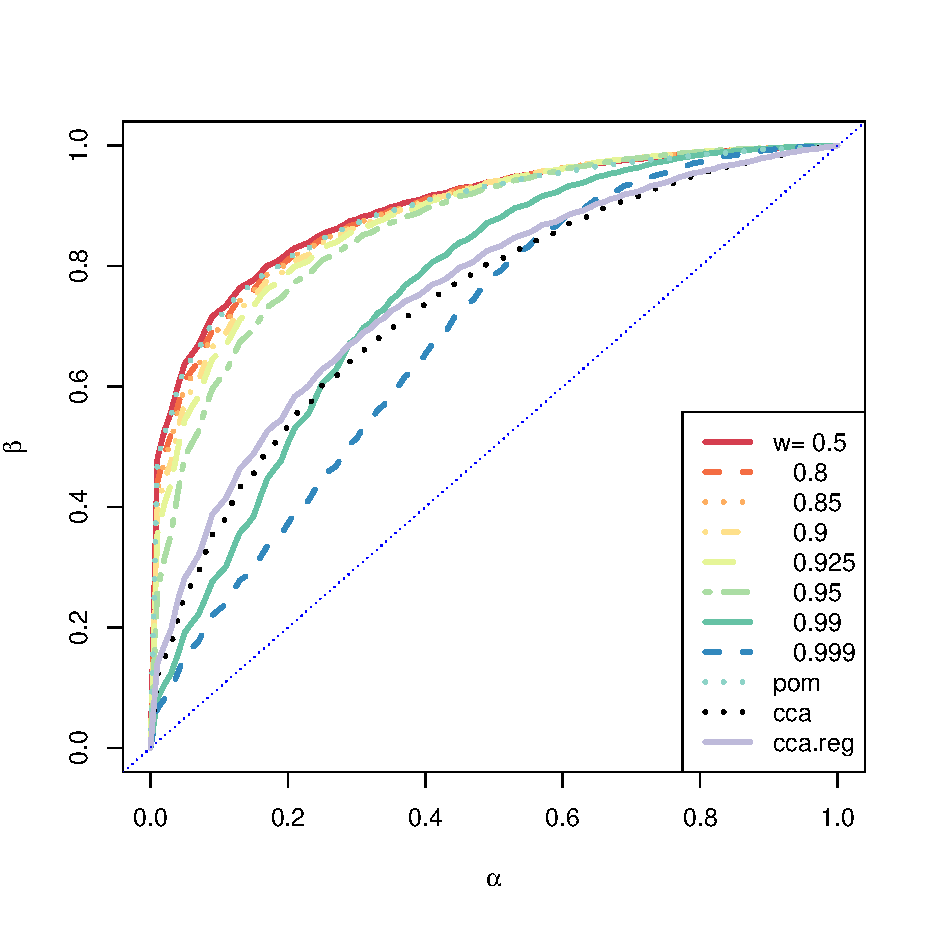
\includegraphics[width=\textwidth]{ROC-d-7.pdf}
                \caption{d=7}
                \label{fig:ROC-d-7}
        \end{subfigure}          
               \begin{subfigure}[b]{0.47\textwidth}
                \centering
               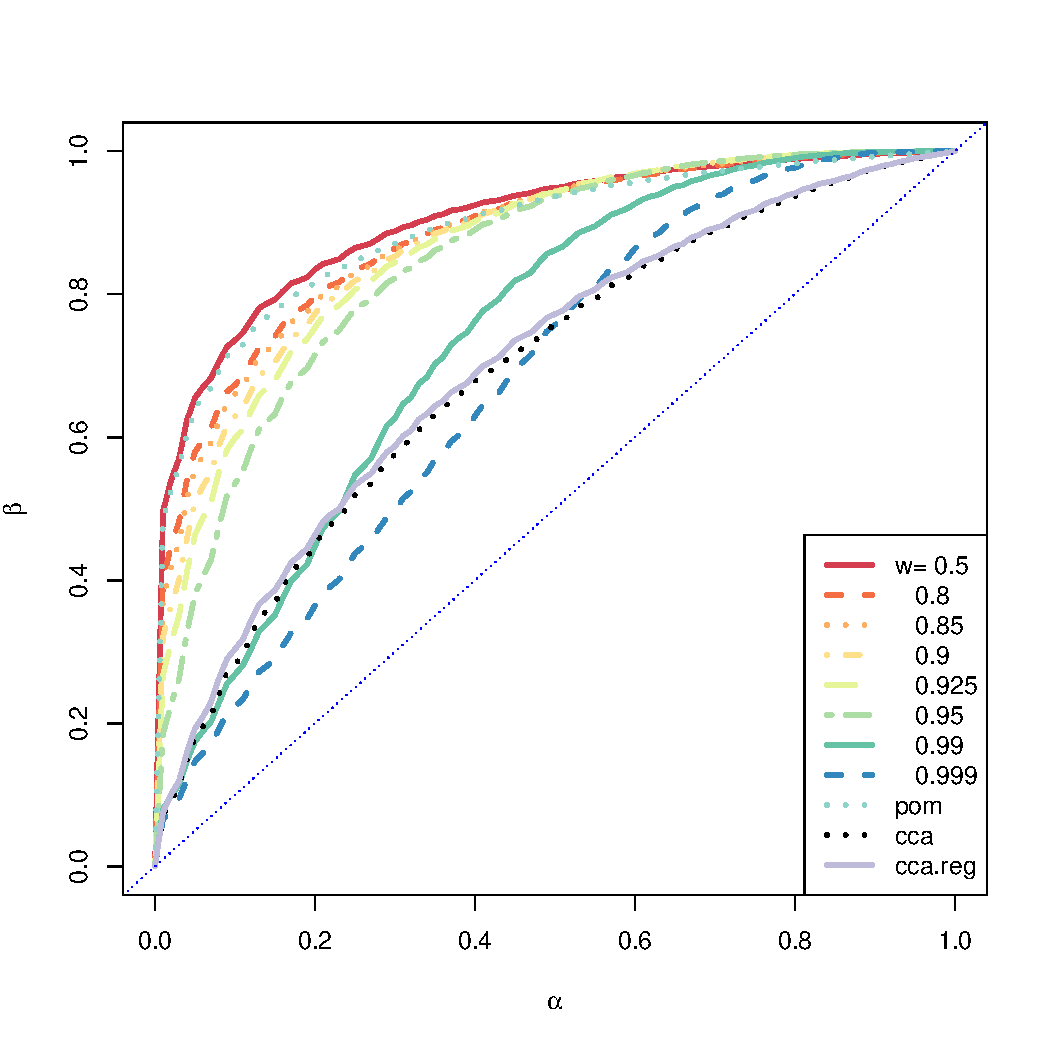
\includegraphics[width=\textwidth]{ROC-d-10.pdf}
                \caption{d=10}
                \label{fig:ROC-d-10}
        \end{subfigure}
         
        \caption{Effect of $d$ parameter on ROC plots}\label{fig:ROC-d}
        \label{fig:ROC-d}

\end{figure}

\begin{center}
\begin{figure}

                \centering
               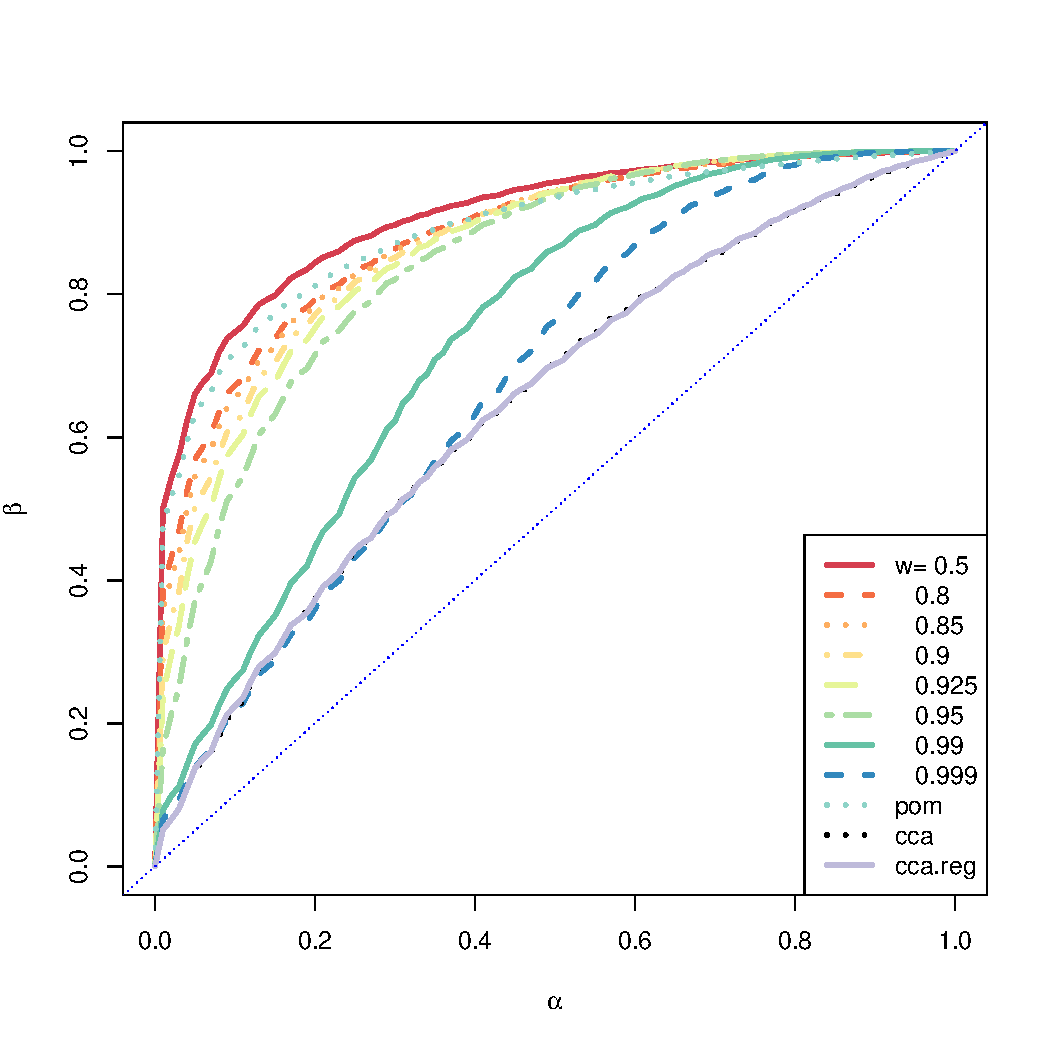
\includegraphics[scale=0.75]{ROC-d-15.pdf}
                \caption{d=15}
                \label{fig:ROC-d-15}
       
\end{figure}
\end{center}


The results show how different approaches are sensitive to the embedding dimension. For larger $d$, CCA and regularized CCA has serious degradation in performance. We expect that this is again due to spurious correlation phenomenon, where more noise dimensions appear in the embedding as the embedding dimension increases. At the same time, the performance of  P$\circ$M and and JOFC with  $w=0.5$  improve with increasing embedding dimension and become the approaches with the best performing test statistic. JOFC with the highest $w$ values ${0.95,0.99,0.999}$  perform slightly worse while the ROC curves for the other $w$ values are more or less the same. Increasing the embedding dimension, seems to push $w^*$ towards the fidelity end ($w=0$) of the fidelity-commensurability tradeoff.
These results require more investigation, so we can  provide a rigorous explanation as to   how the embedding dimension effects the different approaches (JOFC and  P$\circ$M). Specifically, it would help how the null and alternative distributions of the test statistic for the different approaches change with $d$.







\chapter{Seeded Graph Matching and Fast Approximate Quadratic Programming}
\label{sec:sgm-faq}
\chaptermark{Seeded Graph Matching and Fast Approximate Quadratic Programming }

\section{Introduction to Graph Matching}

Another application of  the JOFC approach is  a variant of the graph matching problem. First let us define the general graph matching problem.

 
\subsection{Graph Matching}
Consider two  graphs $G_1=(V_1,E_1)$ and $G_2=(V_2,E_2)$   such that $\| V_1 \|=\| V_2 \|$. Suppose there exists a bijection $f$  between $V_2$ and $V_1$ such that $f(v_2)=v_1$ and $\forall v' \in \mcN(v_2) \textrm{ iff } f(v') \in \mcN(v_1)$. Then the \emph{exact} graph matching problem  is to find $f$. Even the problem of \emph{Graph Isomorphism}, which is defined as determining the existence  of such an isomorphism, is NP-hard.  Although an efficient algorithm  for the general  graph matching problem is not known, there are various principled heuristic algorithms for  approximate solutions of the graph matching problem  in the literature\cite{GraphMatchReview}.
Even though an isomorphism between the two graphs might not exist,  the \emph{approximate} graph matching problem, which is the task of  finding a bijection $f$ between the
graphs which minimizes the degree  of mismatch   between  (edges of ) the two graphs, is an interesting problem  worth studying on its own with practical applications\cite{GraphMatchReview,Bengoetxea2002,recentdevGraphMatching2000,VogConGraphMatchFAQ,Zaslavskiy2009}.


In a specific version of this problem, matchings between some vertices of different graphs are known  and  the  inference task is to infer the correspondences between the remaining collection of vertices in the graphs.  The pairs of vertices whose correspondences are known will be referred to as ``seeds'' and denoted by the pair $(v_2^*,f'(v_2^*)) $  where $v_2^* \in V_2^{*} \subset V_2$ and $f'$ is a bijection between  $V_2^{*}$ and $V_1^{*}\subset V_1$. We will refer to this variant of the graph matching problem as the ``seeded graph matching'' (SGM) problem. These seed pairs provide additional constraints on $\hat{f}$ : $\hat{f}$ must be consistent with the given correspondences, i.e.  $\hat{f}(v_2)=v_1=f'(v_2)\quad \forall v_2 \in V_2^{*} \subset V_2$ and $v_1 \in V_1$. 

Assume $G_1$ and $G_2$ are unweighted graphs\footnote{We should note that most of the notation and methods carry over to the weighted case}. It will be convenient to state the SGM problem in terms of adjacency matrices:

Suppose $A,B \in \mathcal{R}^{(m+s)\times (m+s)}$ are adjacency matrices for graphs $G_1$ and $G_2$
 partitioned as ($m$ rows and then $s$ rows, $m$ columns and then $s$ columns)
\[  A =\left [
\begin{array}{cc} A_{11} & A_{12} \\ A_{21} & A_{22} \end{array} \right ]
\ \ \ \ \ \ \ \ \ B =\left [
\begin{array}{cc} B_{11} & B_{12} \\ B_{21} & B_{22} \end{array} \right ]
\]
Without loss of generality, suppose that $A_{11}=B_{11}$ , \ie the first $m$ vertices
of $A$'s graph correspond respectively to the first $m$ vertices of $B$'s graph,
and we wish to complete the isomorphism by determining the correspondences between the pairs of $s$ vertices. 
That is, we seek a permutation matrix $P \in \{0,1\}^{s \times s}$ such that $A=(I_{m \times m}
\oplus P)B(I_{m \times m} \oplus P)^T$, ie
 \[
 \left [
\begin{array}{cc} A_{11} & A_{12} \\ A_{21} & A_{22} \end{array}
\right ]
\left [
\begin{array}{cc} I_{m \times m} & 0_{m \times s} \\ 0_{s \times m} & P \end{array}
\right ]
=
\left [
\begin{array}{cc} I_{m \times m} & 0_{m \times s} \\ 0_{s \times m} & P \end{array}
\right ]
\left [
\begin{array}{cc} B_{11} & B_{12} \\ B_{21} & B_{22} \end{array}
\right ] 
\].  It is obvious that $P$ determines $f$: $V_2 \rightarrow V_1$, the bijection  between the two graphs we are interested in.

For the approximate graph matching problem, we seek $P$ that minimizes $h(P)$ over all bijective functions, where $h(.)$ measures the mismatch between $G_1$ and $f$ applied to vertices of $G_2$.
For unweighted graphs, the degree of mismatch is characterized by the number of adjacency disagreements, \ie 
$h(P)=\|A- (I_{m \times m}\oplus P)^{T}B(I_{m \times m}\oplus P)\|_1$ subject to $P$ being a permutation matrix.
For weighted graphs, it could be any monotonic transformation of the difference between the weights of correspending edges (lack of edges corresponding to an edge weight of 0).
%
   
   
 Note this optimization problem is equivalent to the minimization of various functions over all permutation matrices $P$,  \eg
 \begin{itemize}
\item $\|A(I_{m \times m}\oplus P)-(I_{m \times m}\oplus P)B\|_1$ (since $I_{m \times m}\oplus P$ is a permutation matrix and the norm is independent of the ordering of the rows and column) or
\item $\|A-(I_{m \times m}\oplus P)B(I_{m \times m}\oplus P)^T\|_2$ (monotonic function of $\ell_1$ norm) or
\item  $\|A(I_{m \times m}\oplus P)-(I_{m \times m}\oplus P)B\|_2$ ( $I_{m \times m}\oplus P$ is unitary), 
 \end{itemize}
or maximizing 
\begin{itemize}
\item $\tr {A^T(I_{m \times m}\oplus P)B(I_{m \times m}\oplus P^T)}$ (expanding out $\|A-(I_{m \times m}\oplus P)B(I_{m \times m}\oplus P)^T\|_2^2=
\|A\|_2^2 + \|B\|_2^2
- 2 \cdot \tr{A^T(I_{m \times m}\oplus P)B(I_{m \times m}\oplus P^T)}$  and removing the constant terms) \label{item:squareofdist_eq_tr_crossprod}
\end{itemize}

where $\| \cdot \|_2$ is the $\ell_2$ vector norm on matrices.   Althought these different formulations  are equivalent, \ie  their global extrema are the same, their relaxations result in different methods for solving the approximate graph matching problem(\autoref{subsec:rqap2}). Specifically the $\ell_1$ formulation is the  linear assignment problem. $\ell_2$ formulations are examples of the quadratic assignment problem.

 
\section{Fast approximate quadratic programming for Seeded Graph Matching}


A relaxation of the general   approximate graph matching problem by letting the  domain of $P$ be doubly stochastic matrices can be solved efficiently by successively solving linearizations of the objective function, the Frank-Wolfe Method. We propose the seeded case version of this relaxation (named as fast approximate quadratic programming)  as the solution to the seeded graph matching problem.
\subsection{Frank-Wolfe algorithm}
A brief review of the Frank-Wolfe algorithm is necessary before we go into FAQ method for Seeded Graph Matching. The F-W algorithm solves the following optimization problem: the minimization of a convex and differentiable function, denoted by $h(x)$ 
over a bounded and convex domain $\mathbf{S}$. 

\begin{algorithm}[H]
 \SetAlgoLined
 %\KwData{this text}
 \KwResult{$x^*$}
 $i=1$\;
 
 $\alpha=1$\;
 
 $x^1$ = Random element of   $\mathbf{S}$  or initial estimate of $\mathit{x^*}$ \;
 
 \While{$\hat{\alpha}>\epsilon $ or $\|\nabla{h(x^{i})}\| > \epsilon$ }{
  Solve $\hat{y}= \argmin_{y}{\nabla{h(x^{i})}}^{T}y$  with respect to  $y$.  
  
 Solve  $\hat{\alpha}= \argmin_{\hat{\alpha}}{h(x^{i}+\alpha*(\hat{y}-x^{i}))}$  with $\alpha \in (0,1)$.
 
  Let $x^{i+1}= x^{i}+\hat{\alpha}*(y-x^{i})$. 
  
  $\mathit{x^*}=x^{i+1}$ 
  
 }
 \caption{Frank-Wolfe algorithm}
\end{algorithm}

The first step in each iteration solves a linear approximation of the problem $h(x)=h(x^i)+\nabla{h(x^i)}(x-x^i)$. The second step minimizes the original function with the domain restricted to the line between $\hat{y}$ and $x^{i}$. When $h(x)$ is quadratic, a unique  $\hat{\alpha}$ can be found analytically.

\subsection{rQAP\textsubscript{1} formulation of Seeded Graph Matching and FAQ Algorithm}
Let us now present the derivation of the steps of  FAQ algorithm.  The objective function we use for FAQ is $\tr {A^T(I_{m \times m}\oplus P)B(I_{m \times m}\oplus P^T)}$. This is a simplified expression for $\ell_2$ distance of $A$ and $(I_{m \times m}\oplus P)B(I_{m \times m}\oplus P)^T$. The feasible region for the optimization is the set of permutation matrices. The minimization of  a cost function over the set of permutations (each one corresponding to an assignment) is known as the quadratic assignment problem. In this case, the cost function has a value of $1$ when the adjacency matrices ($B$ with the vertex labels  permuted and  $A$) agree \ie between two pairs of assigned vertices, there is an edge in one of the graphs and no edges in the other.  The cost function has a value of $0$ when the adjacency matrices disagree.
The relaxation of the optimization where the feasible region is relaxed to the set of doubly stochastic matrices gives our first formulation for the seeded graph matching problem. Therefore we call this formulation relaxed quadratic assignment problem (rQAP\textsubscript{1}).

The objective function is
\begin{eqnarray*}  h(P)  & =  &   \tr \left (
\left [  \begin{array}{cc}  A^T_{11} & A^T_{21} \\ A^T_{12} & A^T_{22}  \end{array} \right ]
\left [  \begin{array}{cc}  I_{m \times m} & 0_{m \times s}
\\ 0_{s \times m} & P  \end{array} \right ]
\left [  \begin{array}{cc}  B_{11} & B_{12} \\ B_{21} & B_{22}  \end{array} \right ]
\left [  \begin{array}{cc}  I_{m \times m} & 0_{m \times s}
\\ 0_{s \times m} & P^T  \end{array} \right ]
\right ) \\
& = & \tr \left (
\left [  \begin{array}{cc}  A^T_{11} & A^T_{21} \\ A^T_{12} & A^T_{22}  \end{array} \right ]
\left [  \begin{array}{cc}  B_{11} & B_{12}P^T \\ PB_{21} & PB_{22}P^T  \end{array} \right ]
\right )\\
& = & \tr A_{11}^TB_{11}+ \tr A_{21}^TPB_{21}+\tr A_{12}^TB_{12}P^T
+ \tr A_{22}^TPB_{22}P^T \\
& = &  \tr A_{11}^TB_{11}+ \tr P^T A_{21}B_{21}^T+\tr P^TA_{12}^TB_{12}
+ \tr A_{22}^TPB_{22}P^T
\end{eqnarray*}
which has gradient $\nabla_{P}(h)$ which is presented  as a matrix-valued function of $P$ as 
\begin{eqnarray*}
\boldsymbol{\nabla}(P):=A_{21}B_{21}^T+A_{12}^TB_{12}+A_{22}PB_{22}^T+A_{22}^TPB_{22} .
\end{eqnarray*} Note that $h(P)$ has a quadratic form with respect to $P$ which will help us with the one-dimensional optimization subproblem in the second step of F-W iterations.


In our experiments,  the Frank-Wolfe Algorithm was initialized with
$\tilde{P}=\frac{1}{s}\vec{1}_{s} \vec{1}_{s}^T$. (This initialization is arbitrary. A random $\tilde{P}$ can be chosen for initializations. Different random initializations would alleviate the local minima problem). 

Now we adapt F-W algorithm to the minimization of $h(P)$.  For each iteration $i$ of the algorithm, in the first step, let $\tilde{P}^{i}$ the current estimate of $P$. We are supposed to compute  $\hat{Q}$ which is the minimizer of  $-\tr Q^{T}\boldsymbol{\nabla}(\tilde{P}^{i})$ over all $s \times s$ doubly stochastic matrices $Q \in \M _{s \times s}$. Equivalently, $\tr Q^{T}\boldsymbol{\nabla}(\tilde{P}^{i})$ is maximized with respect to $Q$. We will use  $\boldsymbol{\nabla}$ in place of the matrix $\boldsymbol{\nabla}(\tilde{P}^{i})$.

 $\hat{Q}$ can be assumed to be a permutation matrix. Birkhoff-von Neumann Theorem\cite{MatrixTheory} states that the set of doubly stochastic matrices is the convex hull of permutation matrices. Since $\tr{Q^{T}\boldsymbol{\nabla}\tilde{P}^{i})}$  is a linear function of $Q$, its maximizer in the convex hull has to be one of the extrema, unless 
%To see this, assume $\hat{Q}$ is not a permutation matrix and there exist a row, say $i^{th}$ row of $\hat{Q}$,named $q_i$, that is not a standard basis of $\R^{s}$($\mathbf{e}_j \in \R^{s}$ with $1$ in $j^{th}$ coordinate, $0$ in other coordinates). Note that the contribution of $q_{i}$ to trace of $Q^{T}G(\tilde{P}^{i})$ is $\sum_{k}{q_{ik}\boldsymbol{\nabla}{}_{ik}}$. Since $\hat{Q}$ is a doubly stochastic  matrix, we also have the constraint $\sum_{k}{q_{ik}}=1$. Of the convex combinations of $\boldsymbol{\nabla}{}_{ik}$, the maximum value achievable is  $\max_k{\boldsymbol{\nabla}{}_{ki}}$ and this maximum is achieved by $q_i=\mathbf{e}_{\argmax_k{\boldsymbol{\nabla}{}_{ki}} }$. As that makes $q_i$ a standard basis $\R^{s}$ , we arrive at a contradiction. 
Thus, $\hat{Q}$  is a permutation matrix and we can limit the feasible region to the set of permutation matrices.
Therefore, the  Hungarian Algorithm which minimizes $-\tr Q^{T}\boldsymbol{\nabla}(\tilde{P}^{i})$ subject to $Q$ being a permutation matrix will in fact find the optimal $Q$, which we denote by $\hat{Q}$.

The next step in the Frank-Wolfe algorithm 
is maximizing the objective function over the line
segment from $\tilde{P}^{i}$ to $\hat{Q}$;  \ie maximizing the scalar-valued univariate function $z(\alpha):=h(\alpha \tilde{P}
+(1-\alpha ) \hat{Q})$ over $\alpha \in [0,1]$. This one-dimensional optimization can be solved with the quadratic formula once the coefficients have been computed. Denote
$$c:=\tr A^T_{22} \tilde{P} B_{22} \tilde{P}^T,\quad d:=\tr (A^T_{22} \tilde{P} B_{22} \tilde{Q}^T +
    A^T_{22} \tilde{Q} B_{22} \tilde{P}^T), \onespace e:=\tr A^T_{22} \tilde{Q} B_{22} \tilde{Q}^T$$ and
$$\quad u:=\tr ( \tilde{P}^TA_{21}B_{21}^T   + \tilde{P}^TA_{12}^TB_{12} ), \quad v:=\tr ( \tilde{Q}^TA_{21}B_{21}^T   + \tilde{Q}^TA_{12}^TB_{12} ).$$ Then
(ignoring the additive constant $\tr A_{11}^TB_{11}$ without loss of
generality)
we have $$z(\alpha)=c \alpha^2+d \alpha (1-\alpha)
+e(1-\alpha)^2+u \alpha + v(1-\alpha)$$  which simplifies to
$z(\alpha)=(c-d+e)\alpha^2+(d-2e+u-v)\alpha + (e+v)$. Setting the
derivative of $z$ to zero yields potential critical point
$\hat{\alpha}:=\frac{-(d-2e+u-v)}{2(c-d+e)}$. We set $\hat{\alpha}:=\min(1,\frac{-(d-2e+u-v)}{2(c-d+e)})$.
%(if indeed $0 \leq \hat{\alpha}\leq 1$). 
If $\hat{\alpha}<\epsilon$, the algorithm terminates at that iteration as  $\hat{P}=\tilde{P}^{i}$  has reached a local minimum. Otherwise, we set $\tilde{P}^{i+1}= \hat{\alpha} \tilde{P}^{i}
+(1- \hat{\alpha} ) \hat{Q}$ if $\hat{\alpha}>\epsilon$   and repeat the steps for the next iteration.

At the termination of the Frank-Wolfe Algorithm, it is quite possible that   $\hat{P}$ is not a permutation matrix. One way to get a permutation matrix solution is to find  ${\tilde{P}}^{*}$ that is as close as possible to  $\hat{P}$ (in some sense). Assume we require the closest permutation matrix in $\ell_2$ sense. Note that in discussion of the different formulations of the  original optimization problem \ref{item:squareofdist_eq_tr_crossprod}, we showed that maximizing $2*\tr {ST}$ with respect to $S$ was equivalent to minimizing $\ell_2$ distance between $S$ and $T$. We have also shown, in the discussion of the FAQ algorithm, minimization of  $2*\tr {ST}$ is solved by the Hungarian algorithm when $S$ is constrained to be permutation matrix. Therefore we can use the Hungarian algorithm one last time to get  the closest permutation matrix to  $\hat{P}$ in $\ell_2$ sense by minimizing $\tr {\tilde{P}}^{*}\hat{P}$ with respect to ${\tilde{P}}^{*}$.

\subsubsection{Demonstration of FAQ on simulated data\label{subsubsec:sgm_sim_results}}

We will demonstrate that  FAQ for SGM works with the following data model:
Let $\G_1=(V_1,E_1)$ be an Erdos-Renyi graph that consists of $n$ vertices and $A$ be its adjacency matrix,  that is
  $\left[A\right]_{ij} \sim \mcB(p)$ where $\left[A\right]_{ij}$ is ${ij}^{th}$ entry of the adjacency matrix  $A$. Another adjacency matrix, $B'$, is a entry-wise bit-flipped version of the adjacency matrix of $A$, that is
    $\{\left[B' \right]_{ij}|\left[A\right]_{ij}=0 \} \sim \Bern(p_{10})$ $\{\left[B'\right]_{ij}|\left[A\right]_{ij}=1 \} \sim \Bern(p_{11})$  . Suppose $p_{10}=p_{11}=p_{pert}$.
    
    Let the isomorphism from  $V_1$ to vertices of the second graph, $V_2$, be denoted by $\psi$. Thus we define the second graph $\G_2=(V_2,E_2)$ with the adjacency matrix $B=P_{\psi}B'P_{\psi}$ where $P_{\psi}$ is the permutation matrix that corresponds to the bijection $\psi$. $m$ ($0\leq m<n$) seeds randomly selected from $n$ pairs of vertices, $\sigma_m \subset V_1$  and  $\{\psi(i), i \in \sigma_m \}\subset V_2 $. The assignment problem for remaining $n-m$ pairs of vertices is solved via FAQ. The quality of the solution to the assignment problem, $\hat{f}_m$ which is a bijection from  $V_1$ to  $V_2$ is evaluated  by  $\delta^{(m)} = \frac{|\{i\in V_1-\sigma_m: \hat{f}_m(i)=\psi(i)\}|}{n-m}$.
  
  The results of our simulations are plotted in the figures \ref{fig:sim_bitflip_rqap_fig1},\ref{sim_bitflip_rqap_fig2},\ref{sim_bitflip_rqap_fig3}. For graph size, we choose $n=600$. We generate pairs of random Erd\o s-Renyi graphs  for different number of seeds, $m$, and  we solve the FAQ problem for the remaining $n-m$ vertex pairs. The probability of flipping an entry of the adjacency matrix is the perturbation parameter $p_{pert}$ which is the variable on the x-axis. The performance measure, the proportion of true matches to the number of matches, is the variable on the y-axis.
  Note that 
  under chance, the expected number of true matches is 1. this means for completely random assignments of vertices, the performance measure of the assignments would be $\frac{1}{n-m}$, as shown with the dashed line.  $p_{pert}$ varies from $0$ to $1$ in increments of $0.1$. 

\begin{figure}[h]
 \centering
  
 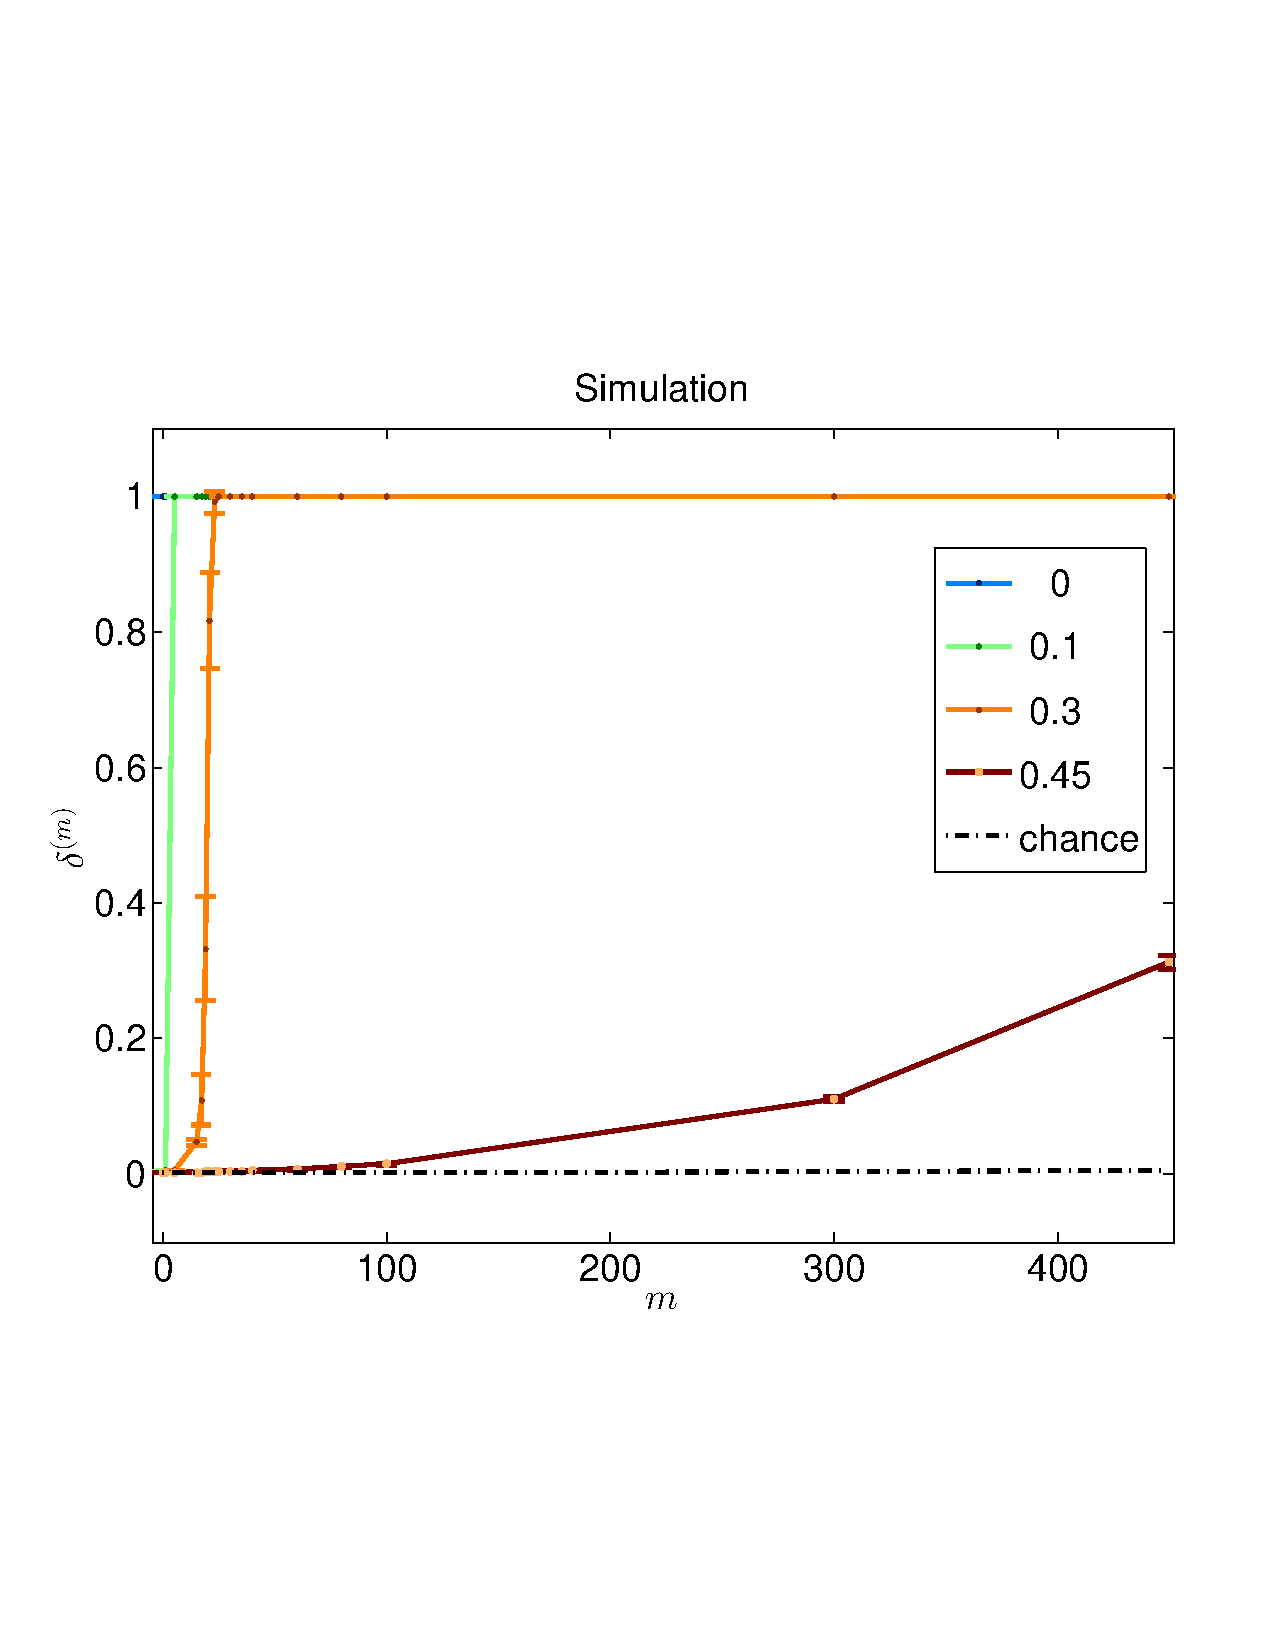
\includegraphics[width=\textwidth]{sim_bitflip-paper600.pdf}
 \caption{$\delta^{(m)}$ vs $m$ for $n=600$ vertices. The error bars represent two times  the standard error of the mean of the true match ratio. Different colors listed in the legend correspond to different $p_{pert}$ values.
 \label{fig:sim_bitflip_rqap_fig1}}
\end{figure}

\begin{figure}
 \centering  
 \includegraphics[width=\textwidth]{sim_bitflip_cluster_300_paper_2.pdf}
 \caption{$\delta^{(m)}$ vs $m$ for $n=300$ vertices. The error bars represent two times  the standard error of the mean of the true match ratio. Different colored lines correspond to different $p_{pert}$ values.
 \label{sim_bitflip_rqap_fig2}}
\end{figure}

\begin{figure}
 \centering
 \includegraphics[width=\textwidth]{sim_bitflip_cluster_300_s_paper_2.pdf}
 \caption{$\delta^{(m)}$ vs $m$ for $n=300$ vertices. This plot includes a  portion of \autoref{sim_bitflip_rqap_fig2} which includes  the x-axis from  $m=0$ to $m=29$. The error bars represent two times  the standard error of the mean of the true match ratio. Different colored lines correspond to different $p_{pert}$ values.
 \label{sim_bitflip_rqap_fig3}}
\end{figure}


\subsection{Relaxations of alternate formulations of \\ the approximate seeded graph matching problem \label{subsec:rqap2}}
There is another quadratic assignment problem formulation of  the approximate seeded graph matching problem, where the objective function is  minimized. We call this formulation rQAP\textsubscript{2}.
The objective function for rQAP\textsubscript{2} is
$\|A\bm{P}-\bm{P}B\|_2^2$ where $\bm{P}=(I_m\oplus P)$. If one applies the constraint of $P$ being an orthogonal matrix, \ie $\|PX\|=\|X\|$ (since the unrelaxed problem requires that $P$ be a permutation matrix, it is also a orthogonal matrix), this objective function simplifies to minimum of -2 times the objective function of  rQAP\textsubscript{1}. The objective function for  rQAP\textsubscript{2} can be simplified as follows:
\begin{align*}
h(P) & = & \lVert A\bm{P}-\bm{P}B\rVert _{F}^2\\
 & = & \underbrace{{\left\Vert A_{21}-PB_{21}\right\Vert _{F}^2}}_{\textrm{Term (1)}} & + & \underbrace{{\left\Vert A_{12}P-B_{12}\right\Vert _{F}^2}}_{\textrm{Term (2)}} & + \underbrace{{\left\Vert A_{22}P-PB_{22}\right\Vert _{F}^2}}_{\textrm{Term(3)} } 
\end{align*}
Consider term (1)
\begin{align*}
\left\Vert A_{21}-PB_{21}\right\Vert _{F} & = & \tr\left[\left(A_{21}-PB_{21}\right)^{T}\left(A_{21}-PB_{21}\right)\right]\\
 & = & \tr\left[A_{21}^{T}A_{21}-B_{21}^{T}P^{T}A_{21}-A_{21}^{T}PB_{21}+B_{21}^{T}P^{T}PB_{21}\right]\\
 & = & \tr\left[A_{21}^{T}A_{21}-B_{21}^{T}P^{T}A_{21}-A_{21}^{T}PB_{21}+P^{T}PB_{21}B_{21}^{T}\right]\\
 & = & \tr\left[A_{21}^{T}A_{21}-2*B_{21}^{T}P^{T}A_{21}+P^{T}PB_{21}B_{21}^{T}\right] \\
 & = & \underbrace{\tr\left[A_{21}^{T}A_{21}\right]}_{(1.1)}
 -\underbrace{2\tr\left[ B_{21}^{T}P^{T}A_{21}\right]}_{(1.2)}
 +\underbrace{\tr\left[P^{T}PB_{21}B_{21}^{T}\right]}_{(1.3)}
\end{align*}
where the simplification in the fourth line is due to the fact that $B_{21}^{T}P^{T}A_{21}$ and $A_{21}^{T}PB_{21}$
 are transposes of each other.
The three terms  in the last line are referred
as (1.1), (1.2) and (1.3), respectively.

We make a similar simplification for term (2):
\begin{align*}
\left\Vert A_{12}P-B_{12}\right\Vert _{F} & = & \tr\left[\left(A_{12}P-B_{12}\right)^{T}\left(A_{12}P-B_{12}\right)\right]\\
 & = & \tr\left[ P^{T}A_{12}^{T}A_{12}P-B_{12}^{T}A_{12}P-P^{T}A_{12}^{T}B_{12}+B_{12}^{T}B_{12}\right]\\
 & = & \tr\left[ PP^{T}A_{12}^{T}A_{12}-B_{12}^{T}A_{12}P-P^{T}A_{12}^{T}B_{12}+B_{12}^{T}B_{12}\right]\\
 & = & \tr\left[ PP^{T}A_{12}^{T}A_{12}-2P^{T}A_{12}^{T}B_{12}+B_{12}^{T}B_{12}\right] \\
 & =  & \underbrace{\tr\left[ PP^{T}A_{12}^{T}A_{12}\right]}_{(2.1)}
 -\underbrace{2 \tr \left[P^{T}A_{12}^{T}B_{12}\right]}_{(2.2)}
 +\underbrace{\tr \left[B_{12}^{T}B_{12}\right]}_{(2.3)}
\end{align*}
The three trace terms will be referred as (2.1), (2.2) and
(2.3), respectively.

Finally, for term (3):
\begin{align*}
\left\Vert A_{22}P-PB_{22}\right\Vert _{F} &=&\tr\left[\left(A_{22}P-PB_{22}\right)^{T}\left(A_{22}P-PB_{22}\right)\right]\\
 &=&\tr\left[P^{T}A_{22}^{T}A_{22}P-B_{22}^{T}P^{T}A_{22}P-P^{T}A_{22}^{T}PB_{22}+B_{22}^{T}P^{T}PB_{22}\right]\\
 &=&\tr\left[PP^{T}A_{22}^{T}A_{22}-B_{22}^{T}P^{T}A_{22}P-P^{T}A_{22}^{T}PB_{22}+PB_{22}B_{22}^{T}P^{T}\right]\\
  &=& {\tr\left[PP^{T}A_{22}^{T}A_{22}\right]}
 - {\tr\left[ B_{22}^{T}P^{T}A_{22}P\right]}\\
 &-&{\tr\left[P^{T}A_{22}^{T}PB_{22}\right]}
 +{\tr\left[ PB_{22}B_{22}^{T}P^{T}\right]}\\
 &=&\underbrace{\tr\left[PP^{T}A_{22}^{T}A_{22}\right]}_{(3.1)}
 -\underbrace{2\tr\left[P^{T}A_{22}^{T}PB_{22}\right]}_{(3.2)}
 +\underbrace{\tr\left[ PB_{22}B_{22}^{T}P^{T}\right]}_{(3.3)}
\end{align*}

The three terms inside the brackets are referred as (3.1),(3.2)  and (3.3)
  respectively.

%Note that $\tr\left[PP^{T}A_{22}^{T}A_{22}-B_{22}^{T}P^{T}A_{22}P-P^{T}A_{22}^{T}PB_{22}+PB_{22}B_{22}^{T}P^{T}\right]$
%can be further simplified to \[
%\tr\left[PP^{T}A_{22}^{T}A_{22}-2*P^{T}A_{22}^{T}PB_{22}+PB_{22}B_{22}^{T}P^{T}\right]
%\]
%.


The gradient for rQAP\textsubscript{2} with hard seeds (minimization problem) is
$\boldsymbol{\nabla}_{P}f(P)=
\underbrace{-2A_{21}B_{21}^{T}}_{(1.2)}
+\underbrace{2PB_{21}B_{21}^{T}}_{(1.3)}
-\underbrace{2A_{12}^{T}B_{12}}_{(2.2)}
+\underbrace{2A_{12}^{T}A_{12}P}_{(2.1)}
+\underbrace{2A_{22}^{T}A_{22}P}_{(3.1)}
+\underbrace{2PB_{22}B_{22}^{T}}_{(3.3)}
-\underbrace{4A_{22}^{T}PB_{22}}_{(3.2)}$. The numbers below the underbraces indicate which term  of $h(P)$ each gradient term comes from.

For the second step of F-W algorithm, we set  $P=(1-\alpha) \hat{P}+ \alpha\hat{Q}$ and maximize $h(P)$ with respect to $\alpha$ for $\hat{Q}$ found in the first step. We will now derive a simplification of this one dimensional optimization problem.

The function in terms of $\alpha$ is
%\begin{flushleft}
\begin{align*}
g(\alpha) & = & \alpha^{2}  \tr\biggl[\hat{P}^{T}\hat{P}\left(B_{21}B_{21}^{T}+B_{22}B_{22}^{T}\right)  & \qquad(1.3+3.3) \\
 &  & +\left(A_{12}^{T}A_{12}+A_{22}^{T}A_{22}\right)\hat{P}\hat{P}^{T} & \qquad (2.1+3.1)\\
 &  &   -2\hat{P}^{T}A_{22}^{T}\hat{P}B_{22}\biggr] & \qquad (3.2)\\ %-\hat{P}^{T}A_{22}\hat{P}B_{22}^{T}
 & +  & \left(1-\alpha\right)^{2}  \tr\biggl[\hat{Q}^{T}\hat{Q}\left(B_{21}B_{21}^{T}+B_{22}B_{22}^{T}\right) & \qquad (1.3+3.3) \\
 &  & +\left(A_{12}^{T}A_{12}+A_{22}^{T}A_{22}\right)\hat{Q}\hat{Q}^{T} &  \qquad (2.1+3.1)\\
 &  &   -\hat{Q}^{T}A_{22}^{T}\hat{Q}B_{22}\biggr] & \qquad (3.2)\\ %-\hat{Q}^{T}A_{22}\hat{Q}B_{22}^{T}
 & + & \alpha\left(1-\alpha\right)  \tr \biggl[ \left(\hat{Q}^{T}\hat{P}+\hat{P}^{T}\hat{Q}\right)\left(B_{21}B_{21}^{T}+B_{22}B_{22}^{T}\right) & \qquad  (1.3)+(3.3) \\
 &  & +\left(A_{12}^{T}A_{12}+A_{22}^{T}A_{22}\right)\left(\hat{Q}\hat{P}^{T}+\hat{P}\hat{Q}^{T}\right)& \qquad (2.1)+(3.1)\\
 &  & -2\hat{P}^{T}\left[A_{22}^{T}\hat{Q}B_{22}\right]-2\hat{Q}^{T}\left[A_{22}^{T}\hat{P}B_{22}\right] \biggr] & \qquad (3.2)\\
 & + & \alpha  \tr\left[-2\hat{P}B_{12}^{T}A_{12}-2\hat{P}^{T}A_{21}B_{21}^{T}\right] &\qquad [-(2.2)-(1.2)]\\
 & + & \left(1-\alpha\right)  \tr\left[-2\hat{Q}B_{12}^{T}A_{12}-2\hat{Q}^{T}A_{21}B_{21}^{T}\right] &  \qquad [-(2.2)-(1.2)]
\end{align*}
%\par\end{flushleft}
where the  numbers in the right end of each line refer to the
terms for corresponding to $\left\Vert A_{21}-PB_{21}\right\Vert _{F}$
,$\left\Vert A_{12}P-B_{12}\right\Vert _{F}^2$ and $\left\Vert A_{22}P-PB_{22}\right\Vert _{F}^2$
in the objective function. Writing $g\left(\alpha\right)$ in terms
of $\alpha$ and (1-$\alpha$),

$g\left(\alpha\right)=c\alpha^{2}+e(1-\alpha)^{2}+d\alpha(1-\alpha)+u\alpha+v(1-\alpha)$


\begin{align*}
c & = &\tr&\left[\hat{P}^{T}\hat{P}\left(B_{21}B_{21}^{T}+B_{22}B_{22}^{T}\right)+\left(A_{12}^{T}A_{12}+A_{22}^{T}A_{22}\right)\hat{P}\hat{P}^{T}-2\hat{P}^{T}A_{22}^{T}\hat{P}B_{22}\right]
\\
d & = & \tr& \biggl[\left(\hat{Q}^{T}\hat{P}+\hat{P}^{T}\hat{Q}\right)\left(B_{21}B_{21}^{T}+B_{22}B_{22}^{T}\right)+\left(A_{12}^{T}A_{12}+A_{22}^{T}A_{22}\right)\left(\hat{Q}\hat{P}^{T}+\hat{P}\hat{Q}^{T}\right) \\
 &  &  & -\hat{P}^{T}\left[2 A_{22}^{T}\hat{Q}B_{22}\right]-\hat{Q}^{T}\left[ 2 A_{22}^{T}\hat{P}B_{22}\right]\biggr] \\
e & =& \tr & \left[\hat{Q}^{T}\hat{Q}\left(B_{21}B_{21}^{T}+B_{22}B_{22}^{T}\right)+\left(A_{12}^{T}A_{12}+A_{22}^{T}A_{22}\right)\hat{Q}\hat{Q}^{T}-2\hat{Q}^{T}A_{22}^{T}\hat{Q}B_{22}\right]
\\ u & = & \tr &\left[-2\hat{P}B_{12}^{T}A_{12}-2\hat{P}^{T}A_{21}B_{21}^{T}\right]
\\ v & = & \tr &\left[-2\hat{Q}B_{12}^{T}A_{12}-2\hat{Q}^{T}A_{21}B_{21}^{T}\right]
\end{align*}

The coefficients of this  polynomial of $\alpha$ in standard form $g(\alpha)= a{\alpha}^2+b\alpha+c$ equal $a=c+e-d$,
$b=d-2e+u-v$ and $c=e+v$ .

Note that if this rQAP\textsubscript{2} formulation is further simplified  by the unitary/orthogonality property of permutation  matrix, we get the first rQAP\textsubscript{1} formulation. When we use the constraints $P^TP=PP^T=I_{s}$, terms (1.3),(2.1),(3.1),(3.3) become constant terms. The corresponding  terms that in $\boldsymbol{\nabla}_{P}f(P)$ vanish,
$\boldsymbol{\nabla}_{P}f(P)=-2A_{21}B_{21}^{T}+2PB_{21}B_{21}^{T}-2A_{12}^{T}B_{12}+2A_{12}^{T}A_{12}P+2(A_{22}^{T}A_{22}P+PB_{22}B_{22}^{T}-2A_{22}^{T}PB_{22})$
becomes $-2*(A_{21}B_{21}^T+A_{12}^TB_{12}+A_{22}PB_{22}^T+A_{22}^TPB_{22})$ which is the gradient for rQAP\textsubscript{1} formulation.
%This can be interpreted as a projection on
%The stronger condition of minimization over the set of permutation matrices is incorporated in the Hungarian Algorithm step.
An interesting question is how does this extra constraint effect the convergence properties of Frank-Wolfe algorithm.  This question is investigated in the comparison of rQAP\textsubscript{1} and rQAP\textsubscript{2} formulations.  

\subsection{The comparison of rQAP\textsubscript{1} against the alternative formulation rQAP\textsubscript{2}}
Although the two formulations are equivalent and the global extrema of the two functions are the same, we expect different convergence  properties. In particular the extra terms in the gradient of rQAP\textsubscript{2} which vanishes for unitary matrices should act as a random noise. The conclusion of the literature of stochastic optimization  is that, under some conditions, such noise speeds up convergence, by overcoming local extrema. However, for convergence of the iterative algorithm , the noise needs to vanish to negligible levels. While the final permutation matrix is orthogonal, the solution of the rQAP\textsubscript{1} is not necessarily orthogonal. So rQAP\textsubscript{2}  will eventually converge to an orthogonal matrix, while rQAP\textsubscript{1}   has no such constraint.

The experiment in the \autoref{subsubsec:sgm_sim_results} was repeated with both rQAP\textsubscript{1} and rQAP\textsubscript{2}. For the same pairs of graphs,  the fraction of nonseed vertices correctly matched were computed for both methods.
%and the fraction of nonseed vertices correctly matched and the average number of iterations to satisfy a stopping criteria was compared between the two formulations. 


\begin{figure}
 \centering
  \caption{ Fraction of correctly matched non-seed vertices for $m$ seeds (x-axis). Different colors correspond to different  $p_{pert}$. Solid and dashed lines corresponds to rQAP\textsubscript{1} and rQAP\textsubscript{2} solutions, respectively, for the matching problem.
 \label{rqap2}}
 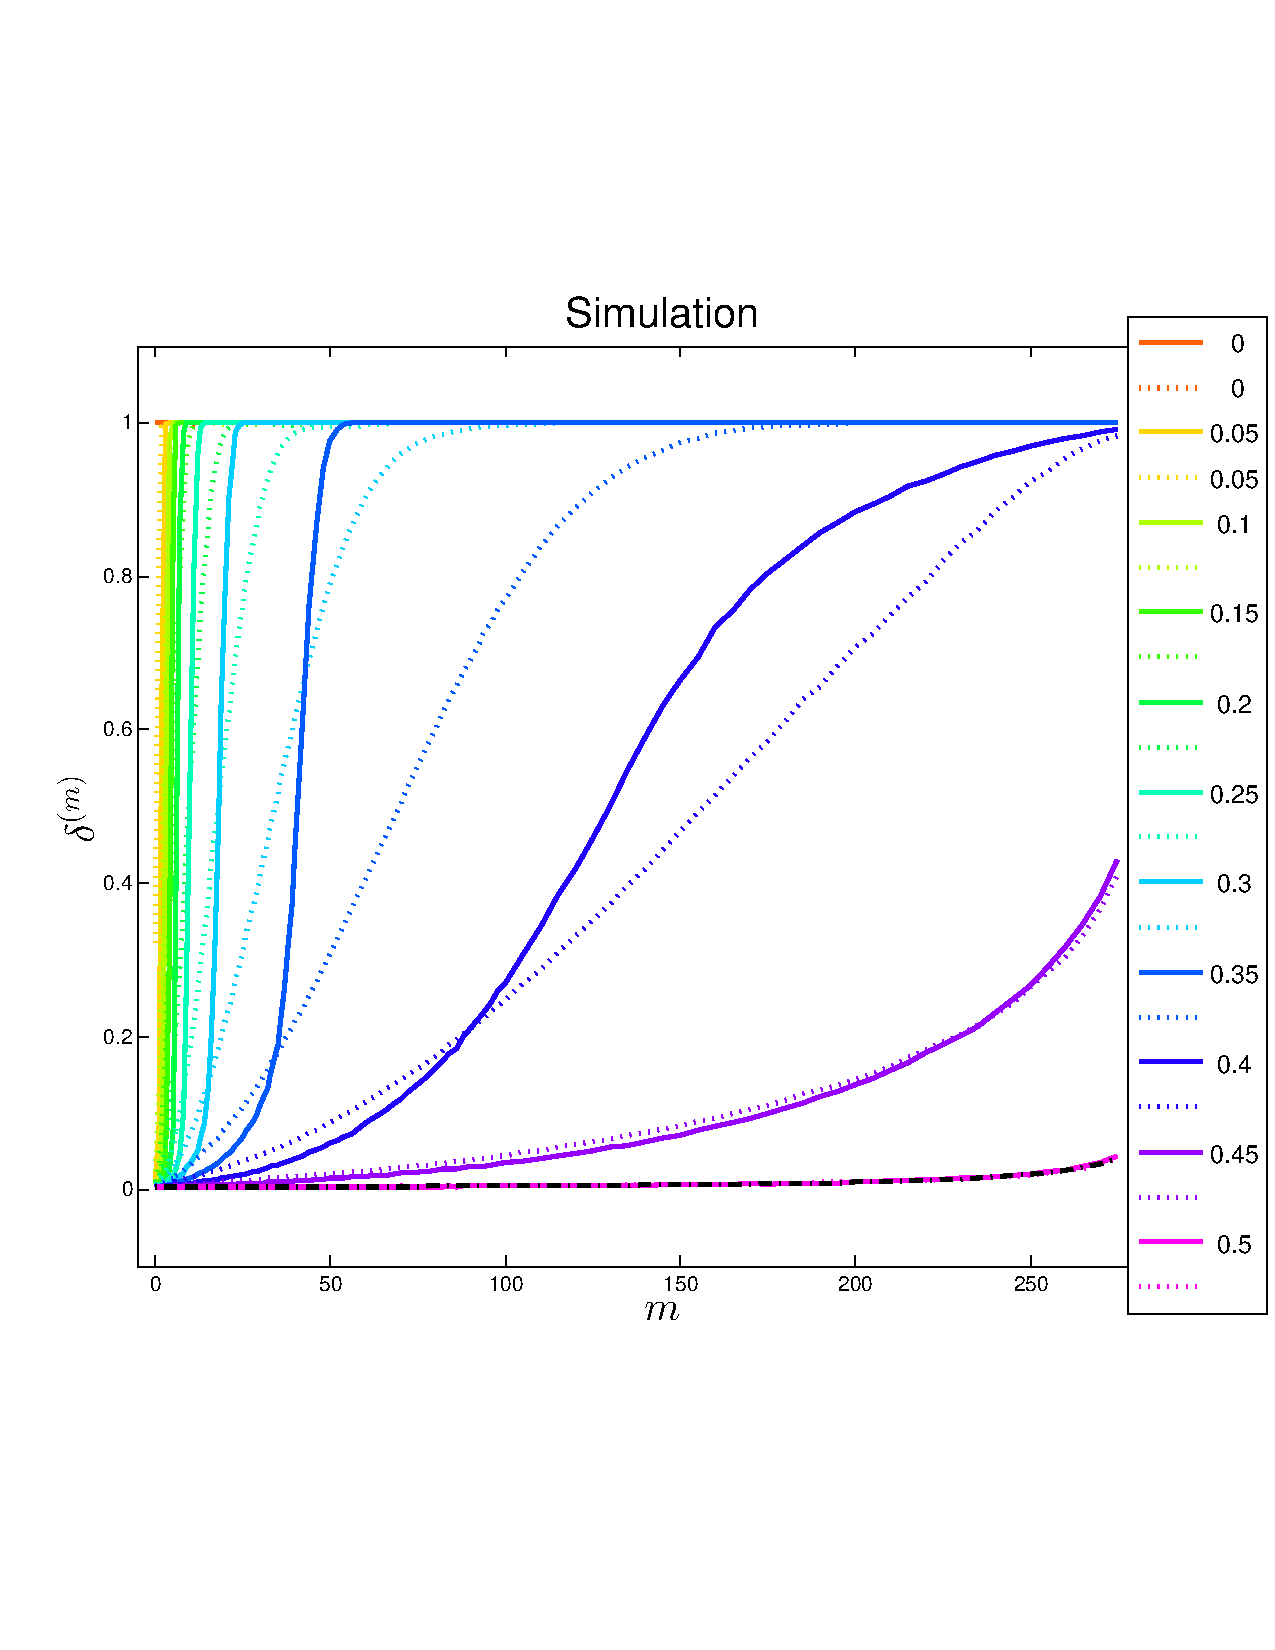
\includegraphics[width=1.2\textwidth]{sim_bitflip_rqap2_300_hsv.pdf}
\end{figure}

\begin{figure}
 \centering
  \caption{Fraction of the $n-m=70$ nonseeds correctly matched using our $\ell_2$-based algorithm for rQAP\textsubscript{1} and rQAP\textsubscript{2} formulations
 \label{figell2}}
 \includegraphics[scale=0.8]{rQAP_vs_rQAP2-alotmore.pdf}
\end{figure}
Note that for small number of hard seeds rQAP\textsubscript{2} is slighly better, while for larger number of hard seeds rQAP\textsubscript{1} is clearly better. The average number of iterations of Frank-Wolfe algorithm until termination for the two formulation is as follows,


Our conclusion is that our expectations for the two formulations is warranted, rQAP\textsubscript{2}   converges slower (or doesn't converge, but stays within the neighborhood of the extrema), while rQAP\textsubscript{1} converges in very few steps. When the number of hard seeds is small (which corresponds to lower number of constraints for P and higher incidence of local minima near the true solution.), rQAP\textsubscript{2} is slightly better than rQAP\textsubscript{1}.


A natural follow-up to the previous inquiry is whether one can get the best of both worlds by making a hybrid of the two formulations: First start with minimizing rQAP\textsubscript{2} function, until the current iterate of solution is relatively close to the true solution, and follow with maximizing rQAP\textsubscript{1} function. 


\subsection{A hybrid formulation: Fast approximate quadratic programming with smooth transition from rQAP\textsubscript{2} to rQAP\textsubscript{1} \label{subsec:hybrid}}

For this hybrid form of the FAQ algorithm, we weight the terms that differ between the gradients of  rQAP\textsubscript{2} and rQAP\textsubscript{1} by a decreasing weight $r$. $\boldsymbol{\nabla}_{P}h(P)=
r*\{2PB_{21}B_{21}^{T}
+2A_{12}^{T}A_{12}P
+A_{22}^{T}A_{22}P
+PB_{22}B_{22}^{T}\}
-2A_{21}B_{21}^{T}-2A_{12}^{T}B_{12}
-4A_{22}^{T}PB_{22}$. As $r \rightarrow 0 $, the gradient expression at each step of F-W algorithm approaches
$-2*(A_{21}B_{21}^T+A_{12}^TB_{12})+A_{22}PB_{22}^T+A_{22}^TPB_{22})$ which is -2 times the gradient in rQAP\textsubscript{1}. We let $r= 0.5- \frac{\tan((i-(i_{end}/2)))}{\pi}$, so as the iteration counter, $i$ goes from $1$ to $i_{end}$, $r$ goes from $1$ to $0$. This hybrid formulation will behave like rQAP\textsubscript{2} for the initial iterations of Frank-Wolfe algorithm and will start to behave like rQAP\textsubscript{1} as $i$ approaches $i_{end}$.


\begin{figure}
 \centering
  \caption{
 \label{fig:hybrid}}
 \includegraphics[scale=0.85]{sim_bitflip_hybrid_cluster_300_hsv.pdf}
\end{figure}



\chapter{JOFC Approach as a solution to Seeded Graph Matching and comparison to FAQ}
\label{sec:sgm-jofc}
\chaptermark{Seeded Graph Matching and JOFC}


Let us first explain the relevance of JOFC to the graph matching problem. The  task of finding vertex correspondences is similar to  detecting matched pairs \ref{chap:match_detection} in that both of the tasks require the quantification of distance between vertex pairs  in the two graphs.
Using omnibus  embedding, it is possible to embed the vertices of two graphs in a commensurate space.
Therefore, the JOFC approach can be used here for determining the pairwise distances in the commensurate space between  the vertices of $A$ and $B$.
The next step is to use the pairwise distances as costs to find the optimal one-to-one matchings by the Hungarian algorithm \cite{Hung-algo}. The Hungarian algorithm finds an optimal matching between two sets of vertices such that the total  cost which is the sum of the pairwise distances of matched nodes is minimized.
%This matching step is separate from the embedding,  we can investigate compare  different parameters for the JOFC approach on a equal footing.

Now, we detail how we use JOFC embedding for seeded graph matching. We begin by jointly embedding our two graphs, $\G_1$ and $\G_2$, into a common Euclidean space. Let $\Delta_1\in \M_{n \times n}$ and $\Delta_2\in \M_{n \times n}$ be two dissimilarity matrices computed by the application of the dissimilarity measure to the vertices of the two graphs. Since we have two separate graphs, we have two conditions and the default assumption is that we do not have  between-graph (between-condition) dissimilarities. We will assume that prior to embedding, the dissimilarities have been normalized to be on the same scale.
%see Remark \ref{rem:norm} for further discussion.

Without loss of generality, we can assume the vertices in both graphs are labeled as integers  from $1$ to $n$, the labeling consistent with the true correspondence  of vertices from different graphs. Suppose we have $m,\, 0 \leq m <n$ seeds. Again, without loss of generality, let the seeded vertices be labeled  as the first $m$ vertices in both graphs, $S_1=\{1,2,\ldots,m\}$ and $S_2=\{1,2,\ldots,m\}$, so that 
$$\Delta^{(1)}=\bordermatrix{&S_{1}&U_{in}\cr
                S_1&\gD^{(1)}_{{in},{in}} 
                & \gD^{(1)}_{{in},2}  \cr
                U_1& \gD^{(1)}_{{oos},{in}}  
                &  \gD^{(1)}_{{oos},{oos}}},\,\,
                \Delta{(2)}=\bordermatrix{&S_2&U_2\cr
                S_2&\gD^{(2)}_{{in},{in}} 
                & \gD^{(2)}_{{in},{oos}}  \cr
                U_2& \gD^{(2)}_{{oos},{in}}  
                &  \gD^{(2)}_{{oos},{oos}}}.$$


Note that the seeds correspond to the in-sample dissimilarities we considered in the match detection task\ref{chap:match_detection} . As these seeds provide the known correspondences (matched observations in the match detection task), we embed them using the in-sample JOFC embedding methodology we introduced in \ref{sec:jointembed}. That is, we find $\X= \begin{array}{c}
\X_1 \\
\X_2
\end{array}$ such that $d(\X)$ is as close as possible to $$M= \begin{array}{cc}
\gD^{(1)}_{in,in} & L \\
 L^T &\gD^{(2)}_{in,in}
\end{array} . $$

The remaining non-seed vertices are embedded using out-of-sample embedding with respect to the embedded seeds, \ie we seek the configuration ${ \hat{\mathbf{Y}}}$ consisting of points in $\mathbb{R}^{d'}$ that consists of the $n-m$ unseeded vertices of $G_1$, with the embedded coordinates  $\{\yhat^{(1)}_{(m+1)},\ldots,\yhat^{(1)}_{(n)}\}$, and the $n-m$ unseeded vertices of $G_2$, with the embedded coordinates  $\{\yhat^{(2)}_1,\ldots,\yhat^{(2)}_{(n-m)}\}$, where $\yhat_{i}^{(k)}, \onespace 1\leq i \leq (n-m), k \in {1,2}$  minimize the stress function:
\begin{align}
\sigma({\bf Y})&=\sum_{s=1}^{m}\sum_{t=m+1}^{n} {W^{(1)}_{in,oos}(s,t-m)  \left(d(X^{(1)}_{s},\yhat_t^{(1)})-\gD^{(1)}_{in,oos}(s,t-m)\right)^2 } \label{eq:oos}\\
&+\sum_{s=m+1}^{n}\sum_{t=1}^{m}
{W^{(2)}_{oos,in}(s-m,t)  \left(d(X^{(2)}_{s},\yhat_t^{(2)})-\gD^{(2)}_{oos,in}(s-m,t)\right)^2}  \label{eq:oos2}\\
&+\sum_{s=m+1}^{n}\sum_{t=1}^{m} 
{W^{(2)}_{oos,oos}(s-m,t-m) \left(d(\yhat_s^{(1)},\yhat_t^{(1)})-\gD^{(1)}_{oos,oos}(s-m,t-m)\right)^2} \label{eq:oos3}\\
&+\sum_{s=m+1}^{n}\sum_{t=1}^{m} 
{W^{(2)}_{oos,oos}(s-m,t-m) \left(d(\yhat_s^{(2)},\yhat_t^{(2)})-\gD^{(2)}_{oos,oos}(s-m,t-m)\right)^2} \label{eq:oos4} \\
&+\sum_{s=m+1}^{n} \sum_{t=1}^{m}
W^{(1,2)}_{oos,oos}(s-m,t-m) \left(d(\yhat_s^{(1)},\yhat_t^{(2)})-\delta(\yhat_s^{(1)},\yhat_t^{(2)})\right)^2 \label{eq:oos5}\\
&+\sum_{s=m+1}^{n} \sum_{t=1}^{m}
W^{(1,2)}_{oos,in}(s-m,t) \left(d(\yhat_s^{(1)},X^{(2)}_{t})-\delta(\yhat_s^{(1)},X^{(2)}_{t})\right)^2 \label{eq:oos6}\\
&+\sum_{s=1}^{m} \sum_{t=m+1}^{n}
W^{(1,2)}_{in,oos}(s,t-m) \left(d(X^{(1)}_{s},\yhat_t^{(2)})-\delta(X^{(1)}_{s},\yhat_t^{(2)})\right)^2 \label{eq:oos7}
%+\sum_{i=1}^{u_1} \sum_{j=1}^{s_2} W^{(1,2)}_{in,oos}(s-m,t) \left(d(Y^{(1)}_i,X^{(2)}_j)-\delta(Y^{(1)}_i,X^{(2)}_j)\right)^2 \\
%&+\sum_{i=1}^{s_1} \sum_{j=1}^{u_2} W^{(1,2)}_{in,oos}(s-m,t-m)\left(d(X^{(1)}_i,Y^{(2)}_j)-\delta(X^{(1)}_i,Y^{(2)}_j)\right)^2, 
\end{align}
%where again $\widetilde w(\cdot,\cdot):V_1\times V_2 \mapsto\mathbb{R}$ are weighting functions representing our confidence in the computed/imputed dissimilarity between pairs of vertices, and as before $\delta$ is the unknown across--graph dissimilarity. 
where $W_{a,b}^{(k)}$ and $W_{a,b}^{(k_1,k_2)}$ (for $a,b \in \{`in', `oos'\}$ are the weights for dissimilarities between in/out-of-sample observations both in $k^{th}$ (or $k_1^{th}$ and $k_2^{th}$) conditions.

Note that \ref{eq:oos5}, \ref{eq:oos6} and \ref{eq:oos7} involve dissimilarities $\delta(.^{(1)},.^{(2)})$ between different conditions, which are generally not available. While  the dissimilarities in \ref{eq:oos6} and \ref{eq:oos7} can be imputed via known dissimilarities, the dissimilarities in \ref{eq:oos5}  cannot be imputed in any way. In fact, if these dissimilarities in  \ref{eq:oos5}   between out-of-sample observations in different conditions were known, we would already know the solution to our inference task, as we would have the  assignment cost  of any oos observation in one condition to another oos observation in another condition and we would minimize the total cost over all possible alignments. In other words, all we would have to do is solve the linear assignment problem).

\ref{eq:oos3} and \ref{eq:oos4} contain dissimilarities between oos observations in the same condition. They can be  used or ignored in the joint embedding, depending on whether one wishes to embed oos observations all together or one at a time. If between-condition oos dissimilarities are ignored, the oos embedding function $\sigma({\bf Y})$ is separable with respect to different  $\yhat^{(k)}_{j} \quad j \in m+1,\ldots n$. Then we would get the same embedding configuration if the oos observations $\yhat^{(k)}_{j}\quad j \in m+1,\ldots n$ are embedded one at a time.

Once we find a minimum configuration ${ \hat{\mathbf{Y}}}$, we compute the pairwise distances between the points $c_{ij}=d(\yhat^{(1)}_s,\yhat^{(2)}_t),\onespace s \in \{(m+1),\ldots n\}, t \in  \{(m+1),\ldots n\}$, which corresponds to the off-diagonal block matrix of $d({ \hat{\mathbf{Y}}})$. This is the assignment cost matrix $C=\left[c_{ij} \right]$ for which we solve the linear assignment problem for which is to minimize $\tr(A^{T}C)=\sum_{ij} a_{ij}*c_{ij}$  for the assignment $\{a_{ij}\}$ where
$\forall i',j' \qquad a_{i'j'} \in {0,1},\onespace \sum_{i}{a_{ij'}} =\sum_{j} a_{i'j} =1 $ \ie $A$ is a permutation matrix. 

So the seeded graph matching problem is solved by a joint embedding of the two graphs followed by solving the linear assignment problem of distances between embedded points.
 
One useful property of dissimilarity representation is that the structure of data is irrelevant once an appropriate dissimilarity function  for the data is available. 
There are many dissimilarities that can be defined between vertices in graphs. We assume that an appropriate dissimilarity measure is available to us.
%See \cite{diffdist}, \cite{dis1}, \cite{dis2} for a wealth of possible dissimilarity measures.  
In our experiments we will use five different dissimilarities/distances between vertices in a graph:
\begin{itemize}
 \item the shortest path on the  unweighted graph whose adjacency matrix is available
 \item the shortest path on a weighted version of the graph whose weight matrix is available
 \item diffusion distance between vertices on the (unweighted) graph.
 \item weighted extension of Czekanowski-Dice dissimilarity\cite{DICE,weightedDICE} which simplifies to the original Czekanowski-Dice dissimilarity in the case of unweighted graphs(C-D dissimilarity  quantifies local similarity of two vertices in a graph).
 \item expected commute time for random walks on the graph.
 \end{itemize}
 %We will omit the results for weighted graph dissimilarities, since they seem to have the same performance as the weighted dissimilarities.
 \begin{remark}
 Note that these dissimilarities are defined between vertices of the same graph. Since the dissimilarities between vertices of different graphs are not available, we have to resort to the same imputation work-arounds  as the JOFC embedding in  \ref{rem:imputationofdiss}.
 %We impute the inter-condition dissimilarities   as described before in section \ref{omnibus}, or ignore them as defined before in \ref{eq:oos}.
 We would again choose 0 for the dissimilarities between matched vertices, then either impute the remaining unknown dissimilarities or ignore them in the embedding.
 \end{remark}
 
 While it is plausible the JOFC approach can also solve the seeded graph matching (SGM) problem, it is not obvious it can compete with the modified FAQ algorithm, specifically formulated to solve the  seeded approximate graph matching problem. Then, why should one choose to use JOFC for SGM? One of the many problems with analysis of real data is that the graph representation of real data is not always well-defined and the correspondence of vertices may be  ambiguous, one-to-many or many-to-many. In such situations, we would prefer a robust algorithm, that would still match seeded graphs with satisfactory performance. Modified FAQ, in the form that we have presented, can not handle such pathologies and significant changes must be made to modified FAQ algorithm before it can handle them. If it turns out that the true match ratios by the assignments given by the JOFC approach is at least as high as the ones given by the modified FAQ algorithm, we can conclude JOFC is reasonably competitive with the modified FAQ algorithm for seeded graph matching. Our simulations using the correlated Erdos-Renyi graphs and experiments with real graph data are tailored for comparison of  the two approaches. We compared the algorithms whenever both of the approaches   are  feasible for the problem size (the running times are acceptable). This application of JOFC for seeded graph matching is  investigated  in \cite{SGMviaJOFC} with simulation and real datasets and some of the same results will be presented in herein.
 

 
 \section{Demonstrations}

We perform SGM simulations with graphs generated according to a paired Erdos-Renyi graph, and experiments on real-life graphs for  both modified FAQ approach and JOFC. The performance measure we consider is the true match ratio: the number of true matchings of vertices  divided by the number of pairs of vertices.

\subsection{Simulations}


  We first present our exploratory simulations to  test the JOFC approach, and figure out what are reasonable choices for  the dissimilarity measure and $w$ (Fidelity-Commensurability tradeoff parameter). We will also  see how sensitive the results are for different choices of the dissimilarity measure and different $w$ values. 
  
  consider the following simulation: $A$ is the adjacency matrix of an Erdos-Renyi graph, \ie
  $\left[A\right]_{ij} \sim Binomial(p)$ where $\left[A\right]_{ij}$ is $ij$-th entry of the adjacency matrix  $A$. The adjacency matrix  $B$ is a entry-wise bit-flipped version of the adjacency matrix of $A$, \ie
    $\left[B\right]_{ij}|\left[A\right]_{ij}=0 \sim Binomial(p_{10})$ $\left[B\right]_{ij}|\left[A\right]_{ij}=1 \sim Binomial(p_{11})$. Suppose $p_{10}=p_{11}=p_{pert}$.
  
  The probability of flipping an entry of the adjacency matrix is the perturbation parameter $p_{pert}$ which is the variable on the x-axis. 
  The performance measure is the proportion of true matches to the number of matches. Note that 
  under chance, the expected number of true matches is 1, as shown with the dashed line. In this particular simulation, we consider the JOFC approach with classical and raw stress variants and compare the performance of each in small graphs. For JOFC with raw stress, we set $w=0.8$. The joint embedding with cMDS is compared with  the JOFC approach, in order to figure out how the performance measure is sensitive to the Fidelity-Commensurability tradeoff. 
  %$r=20$ and $s=5$. 
  $p_{pert}$ varies from $0$ to $1$ in increments of $0.1$.  
  



  

 


\begin{knitrout}
\definecolor{shadecolor}{rgb}{0.969, 0.969, 0.969}\color{fgcolor}\begin{kframe}


{\ttfamily\noindent\bfseries\color{errorcolor}{\#\# Error: cannot change working directory}}

{\ttfamily\noindent\color{warningcolor}{\#\# Warning: cannot open file './JOFC\_MatchDetect/lib/multipleMinimaTest\_fn.R': No such file or directory}}

{\ttfamily\noindent\bfseries\color{errorcolor}{\#\# Error: cannot open the connection}}

{\ttfamily\noindent\itshape\color{messagecolor}{\#\# You're loading optmatch, by B. Hansen and M. Fredrickson.\\\#\#\ \ The optmatch package makes essential use of D. P. Bertsekas\\\#\#\ \ and P. Tseng's RELAX-IV algorithm and code, as well as\\\#\#\ \ Bertsekas' AUCTION algorithm and code.\ \ Using the software\\\#\#\ \ to 'satisfy in any part commercial delivery requirements to\\\#\#\ \ government or industry' requires a special agreement with\\\#\#\ \ Dr. Bertsekas. For more information, enter\\\#\#\ \ relaxinfo() at the command line.}}

{\ttfamily\noindent\color{warningcolor}{\#\# Warning: cannot open file './JOFC\_MatchDetect/lib/simulation\_math\_util\_fn.R': No such file or directory}}

{\ttfamily\noindent\bfseries\color{errorcolor}{\#\# Error: cannot open the connection}}

{\ttfamily\noindent\color{warningcolor}{\#\# Warning: cannot open file './JOFC\_MatchDetect/lib/oosMDS.R': No such file or directory}}

{\ttfamily\noindent\bfseries\color{errorcolor}{\#\# Error: cannot open the connection}}

{\ttfamily\noindent\color{warningcolor}{\#\# Warning: cannot open file './JOFC-GraphMatch/lib/smacofM.R': No such file or directory}}

{\ttfamily\noindent\bfseries\color{errorcolor}{\#\# Error: cannot open the connection}}

{\ttfamily\noindent\color{warningcolor}{\#\# Warning: cannot open file './JOFC-GraphMatch/lib/oosIM.R': No such file or directory}}

{\ttfamily\noindent\bfseries\color{errorcolor}{\#\# Error: cannot open the connection}}

{\ttfamily\noindent\color{warningcolor}{\#\# Warning: cannot open file './JOFC-GraphMatch/lib/diffusion\_distance.R': No such file or directory}}

{\ttfamily\noindent\bfseries\color{errorcolor}{\#\# Error: cannot open the connection}}

{\ttfamily\noindent\color{warningcolor}{\#\# Warning: cannot open file './JOFC-GraphMatch/lib/graph\_embedding\_fn.R': No such file or directory}}

{\ttfamily\noindent\bfseries\color{errorcolor}{\#\# Error: cannot open the connection}}

{\ttfamily\noindent\bfseries\color{errorcolor}{\#\# Error: could not find function "{}ER"{}}}

{\ttfamily\noindent\bfseries\color{errorcolor}{\#\# Error: could not find function "{}omnibusM"{}}}

{\ttfamily\noindent\bfseries\color{errorcolor}{\#\# Error: object 'G.comb' not found}}

{\ttfamily\noindent\bfseries\color{errorcolor}{\#\# Error: object 'Graph.M' not found}}\end{kframe}
\end{knitrout}


\begin{knitrout}
\definecolor{shadecolor}{rgb}{0.969, 0.969, 0.969}\color{fgcolor}\begin{kframe}


{\ttfamily\noindent\bfseries\color{errorcolor}{\#\# Error: could not find function "{}ER"{}}}\end{kframe}
\end{knitrout}



\begin{knitrout}
\definecolor{shadecolor}{rgb}{0.969, 0.969, 0.969}\color{fgcolor}\begin{kframe}


{\ttfamily\noindent\color{warningcolor}{\#\# Warning: there is no package called 'arrayhelpers'}}

{\ttfamily\noindent\bfseries\color{errorcolor}{\#\# Error: could not find function "{}array2df"{}}}

{\ttfamily\noindent\bfseries\color{errorcolor}{\#\# Error: could not find function "{}summarySE"{}}}

{\ttfamily\noindent\bfseries\color{errorcolor}{\#\# Error: could not find function "{}ggplot"{}}}\end{kframe}
\end{knitrout}


Our first observation from the plot is that for low amounts of perturbation, JOFC performs satisfactorily, that is most of the test vertices are matched correctly. Various dissimilarity measures can be chosen for the dissimilarity matrix. The appropriate dissimilarity measure might depend on the degree distribution and the size of the graph. \autoref{fig:JOFC_on_Graphs_Plot} shows some dissimilarity measures result in significantly different behaviour as $p_{pert}$  changes.

 As the perturbation parameter gets larger, (for all dissimilarity measures) the performance  degrades until it is indistinguishable from random chance at $p_{pert}=0.5$. For this $p_{pert}$ value, there is no edge correlation between the two graphs, since the mutual information between $A_{ij}$ and $B_{ij}$ is 0. So at that  $p_{pert}$ value, we expect on average the same number of true matches as random chance. Further $p_{pert}$ means the dissimilarity between truly matched vertices, say  with the shortest path distance as the dissimilarity measure, is even larger than you would expect by chance, which means even less number of true matches.




\begin{knitrout}
\definecolor{shadecolor}{rgb}{0.969, 0.969, 0.969}\color{fgcolor}\begin{kframe}


{\ttfamily\noindent\color{warningcolor}{\#\# Warning: there is no package called 'arrayhelpers'}}

{\ttfamily\noindent\bfseries\color{errorcolor}{\#\# Error: could not find function "{}array2df"{}}}

{\ttfamily\noindent\bfseries\color{errorcolor}{\#\# Error: argument "{}x"{} is missing, with no default}}

{\ttfamily\noindent\bfseries\color{errorcolor}{\#\# Error: object 'nc.cmds.lf' not found}}

{\ttfamily\noindent\bfseries\color{errorcolor}{\#\# Error: object 'nc.jofc.lf' not found}}

{\ttfamily\noindent\bfseries\color{errorcolor}{\#\# Error: object 'nc.jofc.shortpath.lf' not found}}

{\ttfamily\noindent\bfseries\color{errorcolor}{\#\# Error: object 'nc.jofc.shortpath.lf' not found}}

{\ttfamily\noindent\bfseries\color{errorcolor}{\#\# Error: could not find function "{}summarySE"{}}}

{\ttfamily\noindent\bfseries\color{errorcolor}{\#\# Error: could not find function "{}ggplot"{}}}\end{kframe}
\end{knitrout}


JOFC embedding  has significantly better performance compared to cMDS \ref{fig:JOFC_vs_cMDS_on_ER_graph}. 



As $p_{pert}$ approaches $1$, $\G_2$ gets closer to the complement of $\G_1$. An interesting feature of the plot is the U-shape of the curve for some of the dissimilarities. This invariancy with respect to complement of the graph should be investigated further.  



%An interesting trend in the graph is that shortest-path based dissimilarities are an improvement over diffusion-path dissimilarities for perturbation parameter less than 0.5 , but as perturbation parameter increases past 0.5, fraction of correct matches for diffusion distance based dissimilarity recovers, while for other dissimilarities the fraction continues to fall. 

%The dissimilarity type that has the best improvement in performance is JOFC with shortest path distances in weighted graphs(unweighted graphs have similar performance).


\begin{knitrout}
\definecolor{shadecolor}{rgb}{0.969, 0.969, 0.969}\color{fgcolor}\begin{kframe}


{\ttfamily\noindent\bfseries\color{errorcolor}{\#\# Error: could not find function "{}ER"{}}}\end{kframe}
\end{knitrout}



\begin{knitrout}
\definecolor{shadecolor}{rgb}{0.969, 0.969, 0.969}\color{fgcolor}\begin{kframe}


{\ttfamily\noindent\color{warningcolor}{\#\# Warning: there is no package called 'arrayhelpers'}}\begin{verbatim}
##  num [1:11, 1:100, 1:5] 0 0 0 0 0 0 0 0 0 0 ...
## NULL
\end{verbatim}


{\ttfamily\noindent\bfseries\color{errorcolor}{\#\# Error: could not find function "{}array2df"{}}}

{\ttfamily\noindent\bfseries\color{errorcolor}{\#\# Error: object 'nc.jofc.w.lf' not found}}

{\ttfamily\noindent\bfseries\color{errorcolor}{\#\# Error: could not find function "{}summarySE"{}}}

{\ttfamily\noindent\bfseries\color{errorcolor}{\#\# Error: could not find function "{}ggplot"{}}}\end{kframe}
\end{knitrout}


This graph \ref{fig:JOFC-on-ER-Graph-w_param-plot} shows the effect of the weight parameter of stress $w$ on the probability of true matches. We note that in this graph matching setting using the shortest path distance as the dissimilarity measure and for the $w$ values we tested, there is no significant difference between the true matching ratios. This indicates that the choice of the parameter $w$ is not necessarily critical for performance in all data settings. 
%\begin{figure}
%\includegraphics{FidCommPaper-graph-plot-4}
%\end{figure}



\begin{knitrout}
\definecolor{shadecolor}{rgb}{0.969, 0.969, 0.969}\color{fgcolor}\begin{kframe}


{\ttfamily\noindent\bfseries\color{errorcolor}{\#\# Error: could not find function "{}ER"{}}}

{\ttfamily\noindent\bfseries\color{errorcolor}{\#\# Error: could not find function "{}omnibusM"{}}}

{\ttfamily\noindent\bfseries\color{errorcolor}{\#\# Error: could not find function "{}ER"{}}}

{\ttfamily\noindent\bfseries\color{errorcolor}{\#\# Error: could not find function "{}abind"{}}}\end{kframe}
\end{knitrout}


\begin{knitrout}
\definecolor{shadecolor}{rgb}{0.969, 0.969, 0.969}\color{fgcolor}\begin{kframe}


{\ttfamily\noindent\color{warningcolor}{\#\# Warning: there is no package called 'arrayhelpers'}}

{\ttfamily\noindent\bfseries\color{errorcolor}{\#\# Error: object 'nc.jofc.cmds.d' not found}}

{\ttfamily\noindent\bfseries\color{errorcolor}{\#\# Error: object 'nc.jofc.cmds.d' not found}}

{\ttfamily\noindent\bfseries\color{errorcolor}{\#\# Error: object 'nc.jofc.cmds.d' not found}}

{\ttfamily\noindent\bfseries\color{errorcolor}{\#\# Error: object 'nc.jofc.cmds.d' not found}}

{\ttfamily\noindent\bfseries\color{errorcolor}{\#\# Error: could not find function "{}array2df"{}}}

{\ttfamily\noindent\bfseries\color{errorcolor}{\#\# Error: object 'nc.jofc.d.lf' not found}}

{\ttfamily\noindent\bfseries\color{errorcolor}{\#\# Error: could not find function "{}summarySE"{}}}

{\ttfamily\noindent\bfseries\color{errorcolor}{\#\# Error: could not find function "{}ggplot"{}}}\end{kframe}
\end{knitrout}


\autoref{fig:JOFC_on_ER_Graph_d_param-plot} shows that the embedding dimension is a more important concern when the classical MDS embedding is used. For JOFC, even the smallest embedding ($d=4$) dimension is large enough so that significant amount of fidelity  is not  lost which results in mostly accurate matchings of vertices.



There are a lot  of interesting questions to ponder about the number of known correspondences, such as 
\begin{itemize}
\item How many known correspondences are necessary for satisfactory performance for graphs of some fixed size 
\item Are there  any ``elbows'' in the ``match ratio'' vs number of known correspondences curve,  after which the cost of more correspondences are not justified by the accompanying increase in ``match ratio''.
\end{itemize}.
We try to find answers to these questions by using the Erdos-Renyi graph pair model we introduced along with some real-world graphs.

Figure \ref{fig:bitflipJOFC} shows ``match ratio'' plotted against number of ``seeds'' for the bitflip simulations (the data is generated using the Erdos-Renyi graph pair model) using the Czekanowski-Dice dissimilarity measure. These results along with the previous simulations suggest that even with the perturbation, when a portion of the correspondences are known, it is possible to recover most of the remaining correspondences using JOFC embedding of the pair of graphs. We note that the number of correspondence that must be known before the proportion of true matches are satisfactory depends on various factors such as the size and average connectivity of the graphs, the connectivity of the seed vertices, the dissimilarity measure and the amount of perturbation between the two graphs. Further investigations into these factors could be fruitful. 

\begin{figure}
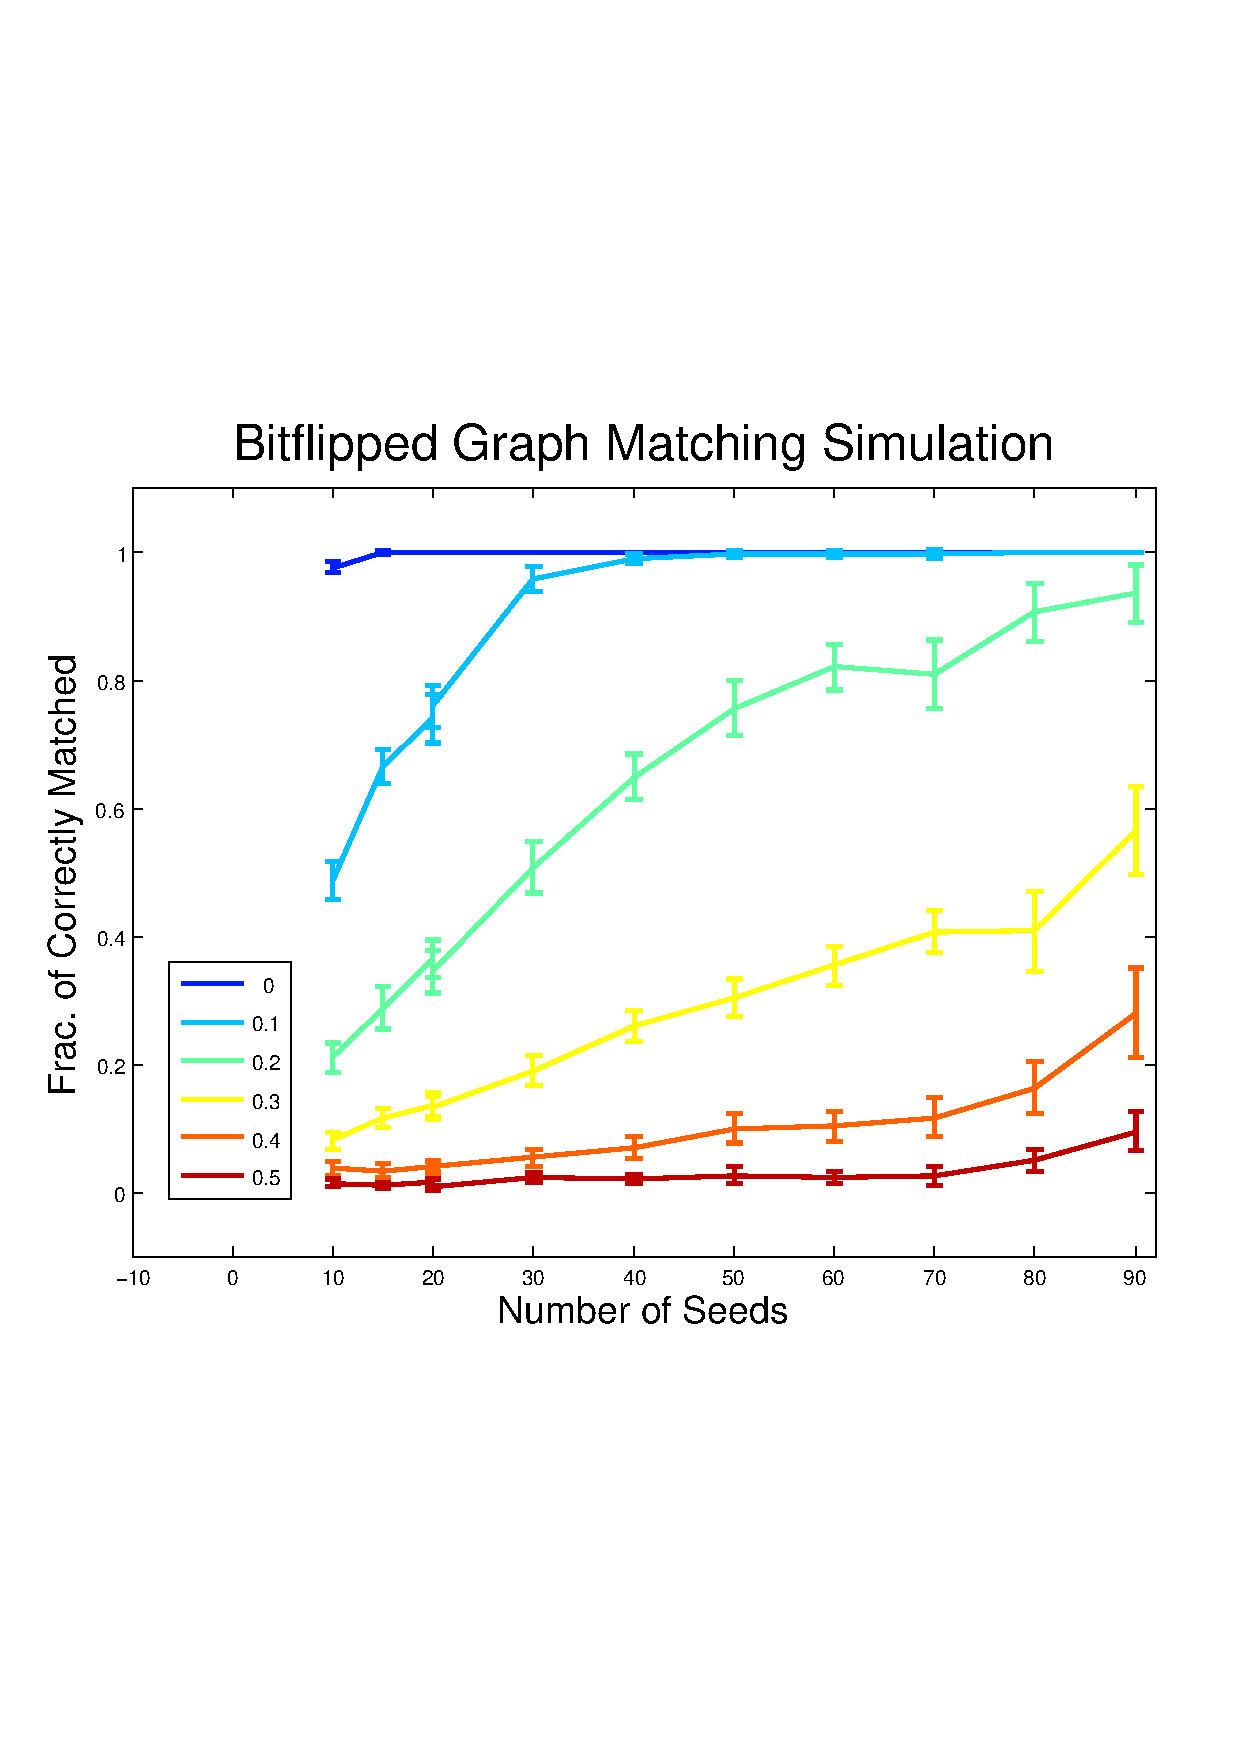
\includegraphics[scale=0.75]{bitflip_JOFC}
\caption{Bitflip Simulations for JOFC \label{fig:bitflipJOFC}}
\end{figure}


\subsection{Experiments on Real data}

\subsubsection{C. elegans connectome}
As one of the real graph data, we consider two connectivity graphs of 279 neurons of the  nematode, \textit{Caenorhabditis elegans}. The two conditions correspond to the two ways of measuring connectivity among neurons $\G_c$ and $\G_g$ . The connectivity in the first connectome is defined by chemical synapses, a directed connection between two cells. This connectome is represented by a weighted graph where the weights correspond to number of synapses identified in images of C. elegans specimens.  The  weight matrix for the first connectivity type is $A_c$ which is not symmetric, has values between 0 and 37 and is relatively sparse (has 2194 non-zero entries). The second connectivity type forms a unweighted graph $\G_g$ with the adjacency matrix $A_g$ and is defined by the existence of gap junctions between neurons. $\G_g$ is even sparser(1031 non-zero entries) than $\G_c$.

We remove isolated vertices from the two graphs and keep vertices which are connected in both graphs. This leaves $n=253$  vertices. We consider both the original weighted graph for the first connectome and binarized version of the same graph. We  also consider symmetrized versions of each graph (which leads to directed and undirected graphs, respectively). In the case of weighted graphs, we normalize the two graphs, so that they approximately have the same scale. For the JOFC approach, we use the weighted DICE dissimilarity (which simplifies to the generic DICE dissimilarity in the case of unweighted graphs) to compute $\Delta_c$ and $\Delta_g$.   

\begin{figure}
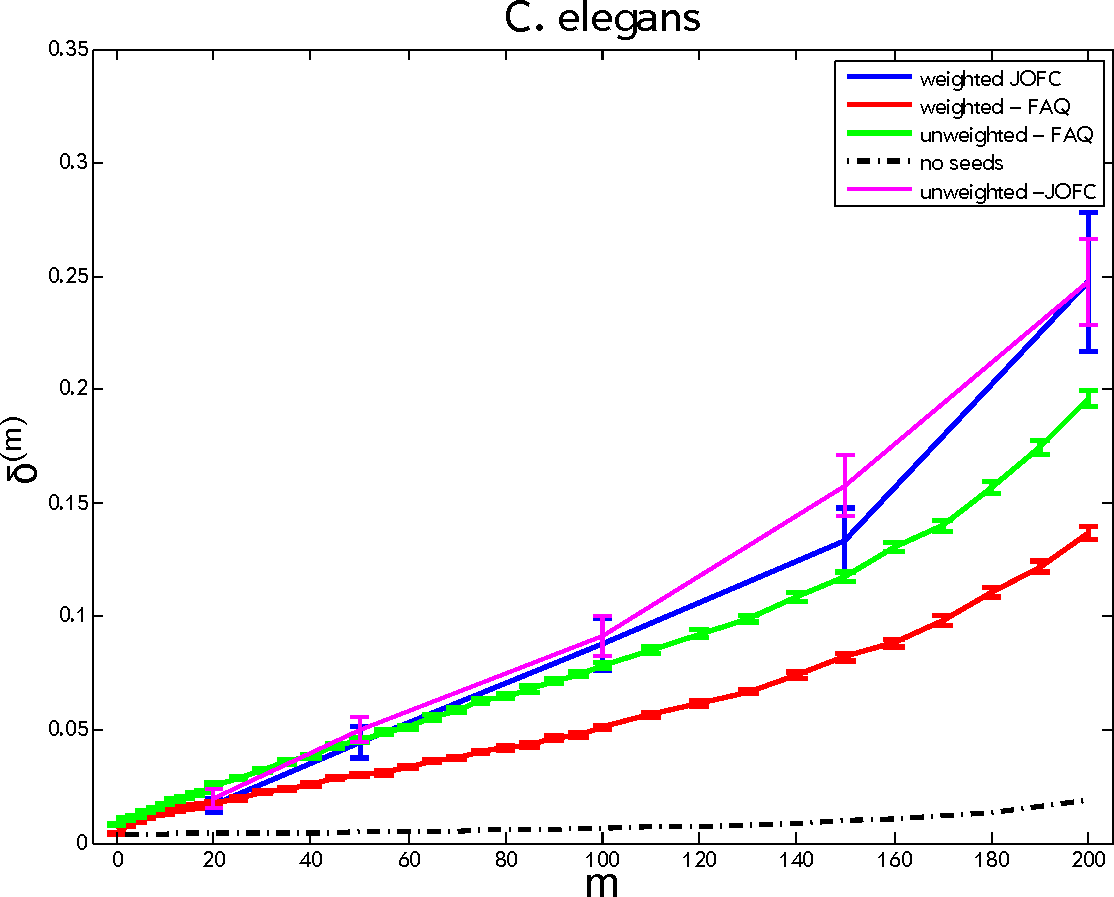
\includegraphics[scale=0.75]{worm_jofc_vs_faq_wt_unwt-crop}
\caption{Graph Matching experiments on the C. elegans connectomes using JOFC and FAQ algorithms \label{worm_graphmatch}}
\end{figure}

We make  a comparison of the JOFC approach and the modified FAQ algorithm using the two connectomes. While the true matching ratio ($\delta^{(m)}$) of both approaches is helped by the number of seeds,  $\delta^{(m)}$ are relatively low compared to the maximum possible value ($1$). This means that the correlation between the two connectomes is small and we expect there are biological explanations for this conclusion.  
The first conclusion we can reach from the comparison is that the two approaches are competitive. In fact, the JOFC approach provide significant improvement over the modified FAQ algorithm. The modified FAQ algorithm is not suitable for the situation when one graph is weighted, and the other graph is unweighted (as in the weighted case) or the number of non-zero entries are significantly different as in this case (as in both the weighted or unweighted cases). JOFC approach works much better in both weighted or unweighted cases. 

\subsubsection{Enron communication graph}
The Enron communication graph is extracted from the  Enron  email corpus, which was made public during criminal investigations by the  Federal Energy Regulatory Commission. Though the number of actual users is about 150,  each email alias is considered as a vertex in the communication graph. The original number of email aliases is 184. The whole time interval is divided into 187 sub-intervals (each corresponding to a week). The emails are grouped according to which time interval their timestamps are in. We then construct a time series of graphs $\mathfrak{G}=\{G^{(t)} = (V,E^{(t)})\}$ where $E^{(t)}$ correspond to emails that were sent at $t^{th}$ interval. We are interested in the intervals $t=130$ , $t=131$ (and $t=132$ for some experiments), as previous  investigations of the corpus found chatter anomalies at these time intervals \cite{EnronStudy}. When isolated vertices (and their corresponding vertices in the other graph) are removed in these two graphs, the number of vertices is reduced to 146. It is these pruned graphs we match. The first two results are from matching of $G(130)$ and $G(131)$. We consider both the undirected and directed versions of the two graphs.


\begin{figure}
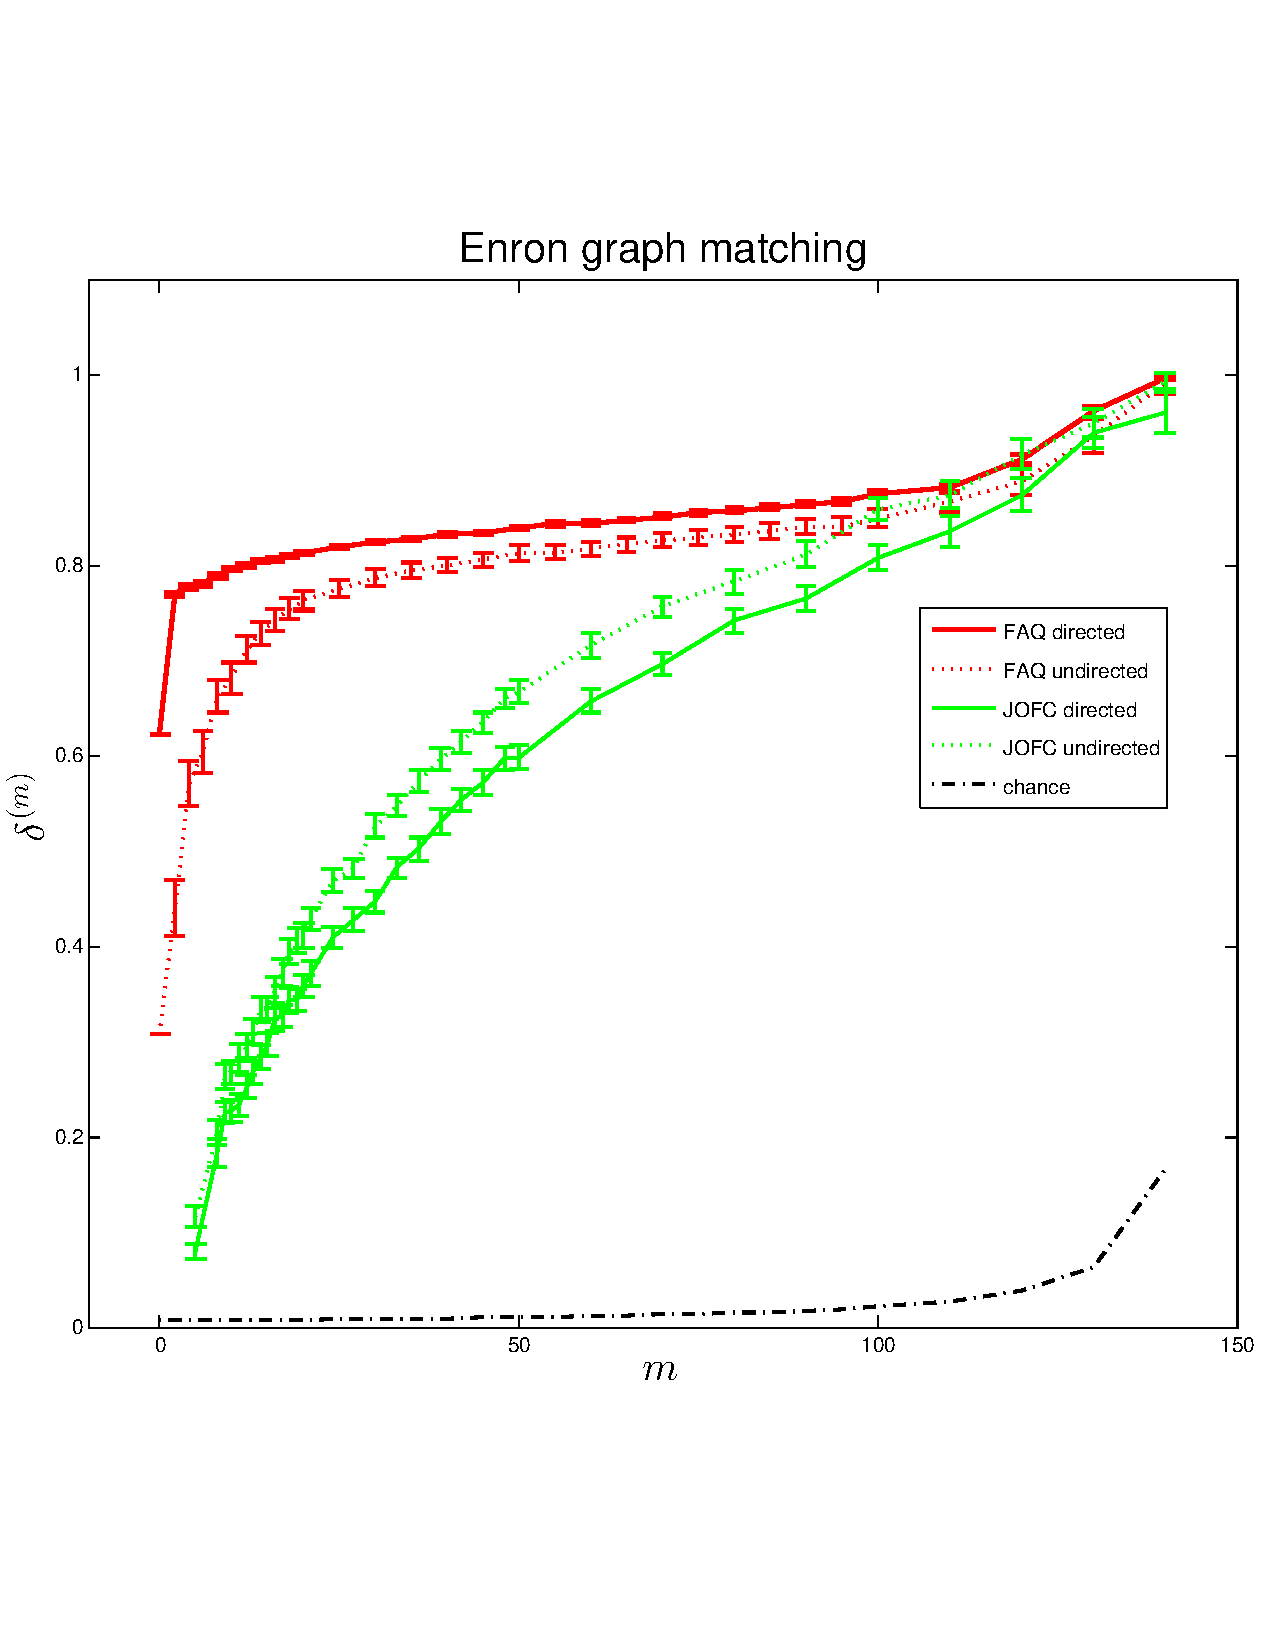
\includegraphics[scale=0.75]{enron-JOFC-FAQ-paper.pdf}
\caption{Experiments on the Enron communication graphs for FAQ and JOFC \label{enron_graphmatch_faq_jofc}}
\end{figure}

We compare the performance of the modified-FAQ algorithm with the JOFC algorithm\ref{enron_graphmatch_faq_jofc}. Here the modified-FAQ algorithm is significantly better than JOFC. This observation  is valid for both directed and undirected versions of the graphs.  With a large  number of seeds, the difference between the two approaches gets smaller. We also note that the performance with the directed graphs is higher than for the undirected graph for the modified FAQ algorithm, while for the JOFC approach  results are   the undirected graph.

\begin{figure}
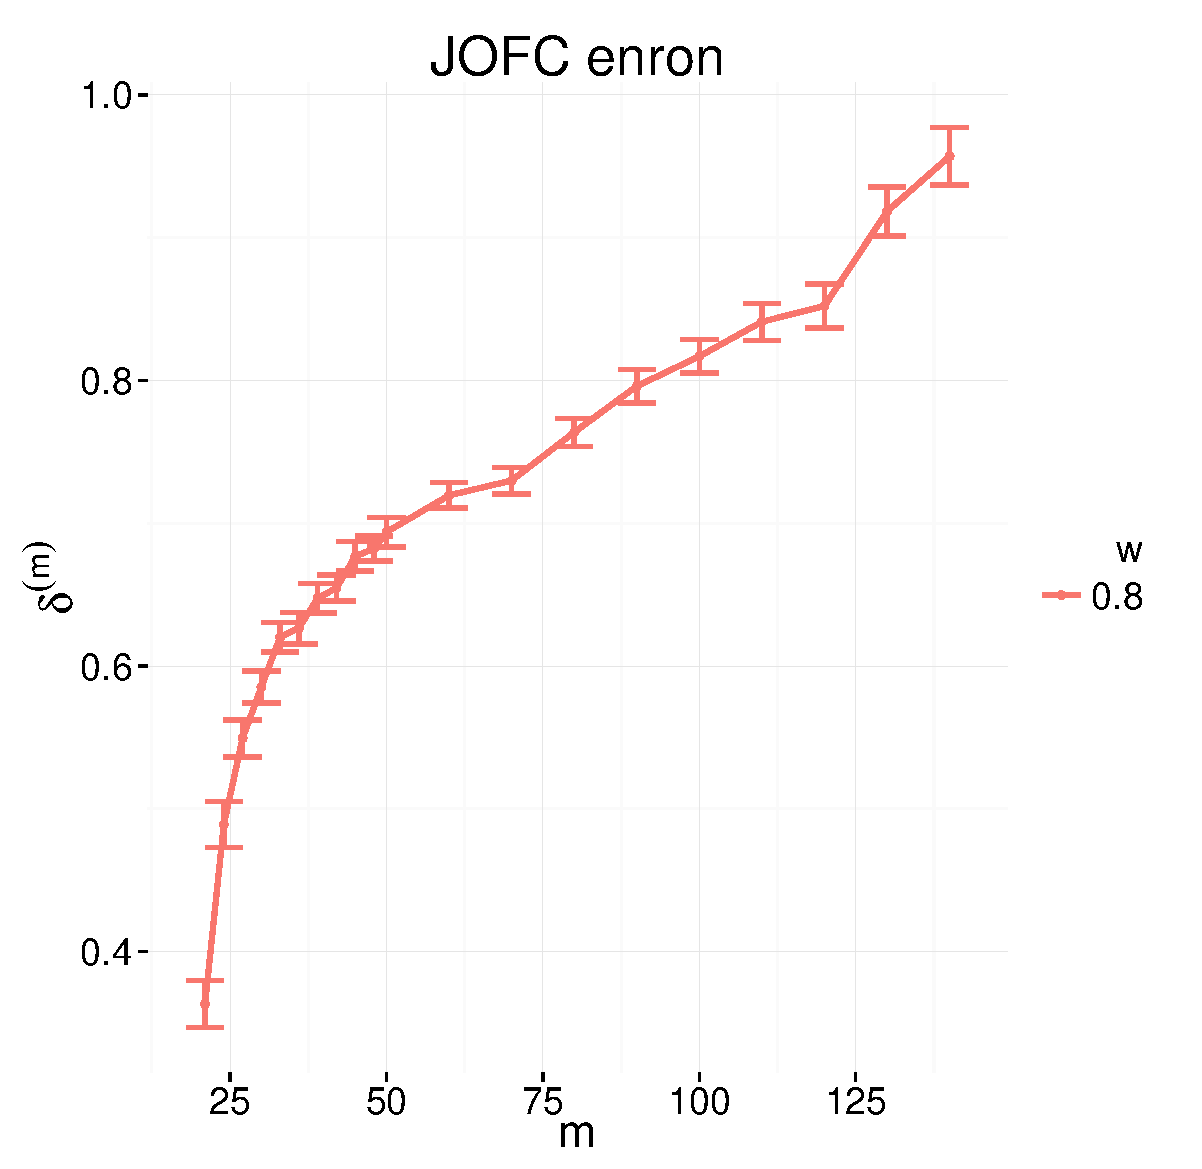
\includegraphics[scale=0.75]{JOFC-enron_dim_20}
\caption{Experiments on the Enron communication graphs for JOFC \label{enron_graphmatch}}
\end{figure}

For the plot in  $\ref{enron_graphmatch}$, we chose the embedding dimension $d$ as 20. These results are better compared to \label{enron_graphmatch_faq_jofc} which leads us to conclude that $d$ is another parameter that must be chosen with care. 


\begin{figure}
\includegraphics[scale=0.75]{enron-paper.pdf}
\caption{Experiments on the Enron communication graphs for FAQ for t=130,131,132 \label{enron_graphmatch_faq_t}}
\end{figure}
The plot in \autoref{enron_graphmatch_faq_t} is another result for matching the Enron graphs using the FAQ algorithm. The comparison of the three pairs from $t=130,131,132$. As one would expect the graph matching between $G(130)$ and $G(131)$ is much more successful than    the graph matching between $G(130)$ and $G(132)$. We also note that if enough seeds are available even the matching between  $G(130)$ and $G(132)$ can be improved significantly . In fact the improvement in the graph matching between  $G(130)$ and $G(132)$  is larger than for the graph matching of the other two pairs.

We are also interested in the chatter anomaly detected in \cite{EnronStudy}. This anomaly is detected at $t=132$. We also see from the graph matching results that the matching between $t=130$ and $131$ is better than the matching between $G(131)$ and $G(132)$. If there is excessive change in the connectivity, we expect the graph matching performance to suffer. This makes one wonder if the true match ratio can be used for detecting anomalies in a time series of graphs. Graph matching can be carried out for the graph instances at consecutive time steps, and significant outliers would be labeled as outliers. The true matching ratio  for a fixed number of seeds would be a statistic for anomaly detection. 

\subsubsection{Wikipedia hyperlink subgraph}

Wikipedia is a free online encyclopedia created by volunteers around the world consisting of millions of article in hundreds of languages (30 million articles in 287 languages, including over 4.3 million in the English Wikipedia as of November 2013 \cite{wikipedia}). Articles contain text, links to other articles and multimedia content. We interpret the links as directed edges in a hyperlink graph where vertices correspond to articles. A collection of articles were collected from the English Wikipedia, consisting of the
 directed 2-neighborhood of the document "Algebraic Geometry"\cite{wikiwebpage}. 
   This  collection of 1382 articles and the correspondence of each article in French 
Wikipedia is our real-life dataset. For inference tasks, it is possible to utilize both textual content of the documents and the hyperlink graph structure. The textual content of the documents is summarized by the bag-of-words model. Dissimilarities between documents  in the same language are computed by the Lin-Pantel discounted mutual information \cite{LinPantel,PantelLin}
 and cosine dissimilarity $k(x_{ik}; x_{jk}) = 1 - (x_{ik} x_{jk})/(\|x_{ik}\|_2\|x_{ik}\|_2)$. 
 The dissimilarities based on the hyperlink graph are shortest path distances in the graph:
 for each pair of vertices $i$ and $j$, the number of vertices one must travel to go from $i$ to $j$. Due to the fact the French Wikipedia graph is sparser, the induced graph in French Wikipedia of 2-neighborhood in English Wikipedia might be a disconnected graph. Therefore the shortest path dissimilarities in French Wikipedia are set to 6 (maximum shortest path distance in English Wikipedia graph), if they are larger than 6.  Further details about this dataset is available in \cite{Zhiliang_disparate}.
 
 As this graph is relatively large compared to other real life graphs we considered, we only tested modified FAQ algorithm. Note that testing JOFC on this graph is still possible, but we had no reason to believe that another JOFC experiment would provide any new insight.

\begin{figure}
\includegraphics[scale=0.75]{wiki-all-with-unseeded.pdf}
\caption{Graph Matching Experiments on the English and French Wikipedia subgraph for FAQ \label{wiki_graphmatch}}
\end{figure}

The results show that there is strong correlation between the two wikipedia graphs, and as many as 50 seeds is enough to improve graph matching dramatically. More seeds improve the true matching ratio,  but the improvements are much more modest. With graph matching using no seeds, we get a very small number of  true matches. 
%The different values plotted in   \ref{wiki_graphmatch} for the no seed case are just independent repeat
      
\subsubsection{Charitynet graph}

The charitynet dataset consists  of timestamped donation relationships between 8052 donors and 756 charities. The donations are divided into two time intervals according to whether they are before the midpoint of the earliest and latest timestamps.
Let $tmid = \frac{(tmax - tmin)}{2}$.
We build two bipartite graphs represented by $B_1$ and $B_2$ for $\left[tmin,tmid\right)$ and $\left(tmid,tmax\right]$, respectively --
each $B^{(t)}$ is $n \times m$, where $n$ is total number of donors in all of charitynet and $m$ is total number of charities in all of charitynet.
so $B_{ij}^{(t)}$ is a 1 if donor $i$ gives to charity $j$ during time interval $t$.

For charities $i$ and $j$,
let $A_{ij}^{(t)}= \sum_{k}{(B_{ik}^{(t)}B_{jk}^{(t)}}$, i.e. the number of donors that both $i$ and $j$ receive from during time interval $t$.
We match the two graphs represented by  $A^{\left[ tmin,tmid \right)}$, $A^{\left(tmid,tmax\right]}$.

\begin{figure}
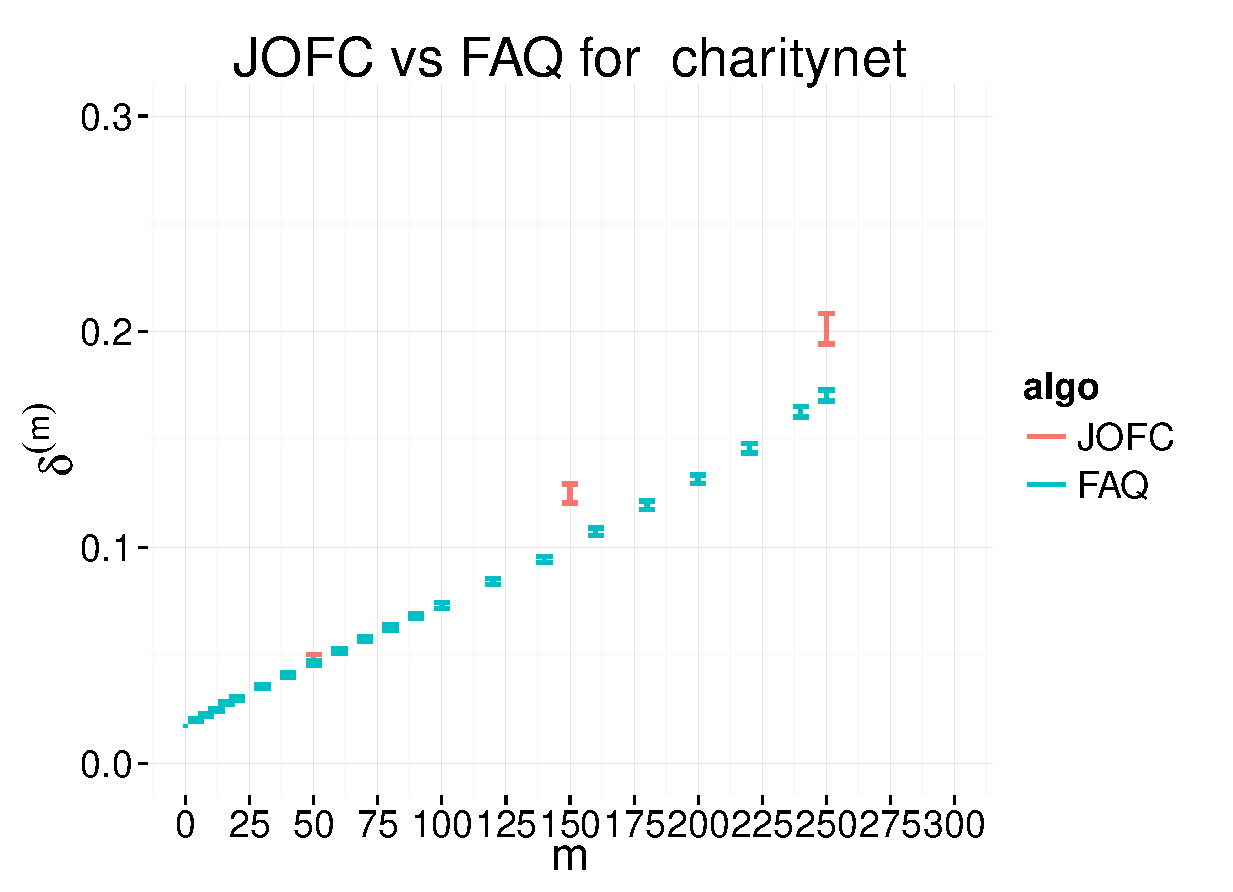
\includegraphics[scale=0.4]{charitynet_SGM_JOFCvsFAQ}
\caption{Graph Matching experiments on the two Charitynet graphs for JOFC \label{charitynet_graphmatch}}
\end{figure}

\subsection{One-to-$k$ matching of vertices} 

Consider the case where the correspondences between vertices of $\G_1=(V_1,E_1)$ and $\G_2= (V_2,E_2)$ (represented by adjacency matrices, $A$ and $B$ respectively) are not one-to-one. To describe the problem in its most general form, we could define group assignment functions $g_1{v_1}: V_1 \rightarrow \mcG={l_1,l_2,\ldots,l_{\upsilon}}$, $g_2{v_2}:V_2 \rightarrow \mcG$ where the inverse images of $g_1{l_i}$, $g_2{l_i}$ are always nonempty. A vertex $v_1 \in  V_1$ in one graph corresponds to a vertex $v_2 \in  V_2$  in another graph, if $g_1(v_1)=g_2(v_2)$. We want to make the simple restriction that $g_2$ is a one-to-one mapping, that is each vertex in $\G_2$ correspond to at least one vertex in  $\G_1$.
For simulations, we consider a very simple case where the $i^{th}$ vertex in $B$ corresponds to $k_i$ vertices in $A$ where $1\leq k_i \leq k_{max}$ where $k_{max}$ is the maximum number of corresponding vertices a $B$ vertex can have.  Denote by $g(\cdot)=g_2^{-1}\circ g_1(\cdot) : V_1 \rightarrow V_2$ the correspondence function from vertices in $\G_1$ to vertices in $\G_2$. Given $r$ vertices in $B$, and the corresponding vertices in $V_1$ for each of the $r$ vertices ($u \in V_1$ such that $g(u)=v_2$), the task is  to find at most $k_max$ closest matches to each vertex of of $\G_2$. 

These three information retrieval performance measures are used: Precision, Recall and F-measure.
$$\mathrm{Precision} =\frac{\textrm{Number of correct matches found}}{\textrm{Number of found matches}}$$
$$\mathrm{Recall}    =\frac{\textrm{Number of correct matches found}}{\textrm{Number of true matches}}$$

$$F-measure  =\frac{2 \times \textrm{Precision} \times \textrm{Recall}}{\textrm{Precision} + \textrm{Recall}}$$

For each vertex of $\G_2$, the number of true matches is $k_i$. The three performance measure is calculated for each vertex of $\G_2$ and then the three averages over all vertices $B$ is the performance measures computed for the  matching.

\begin{figure}
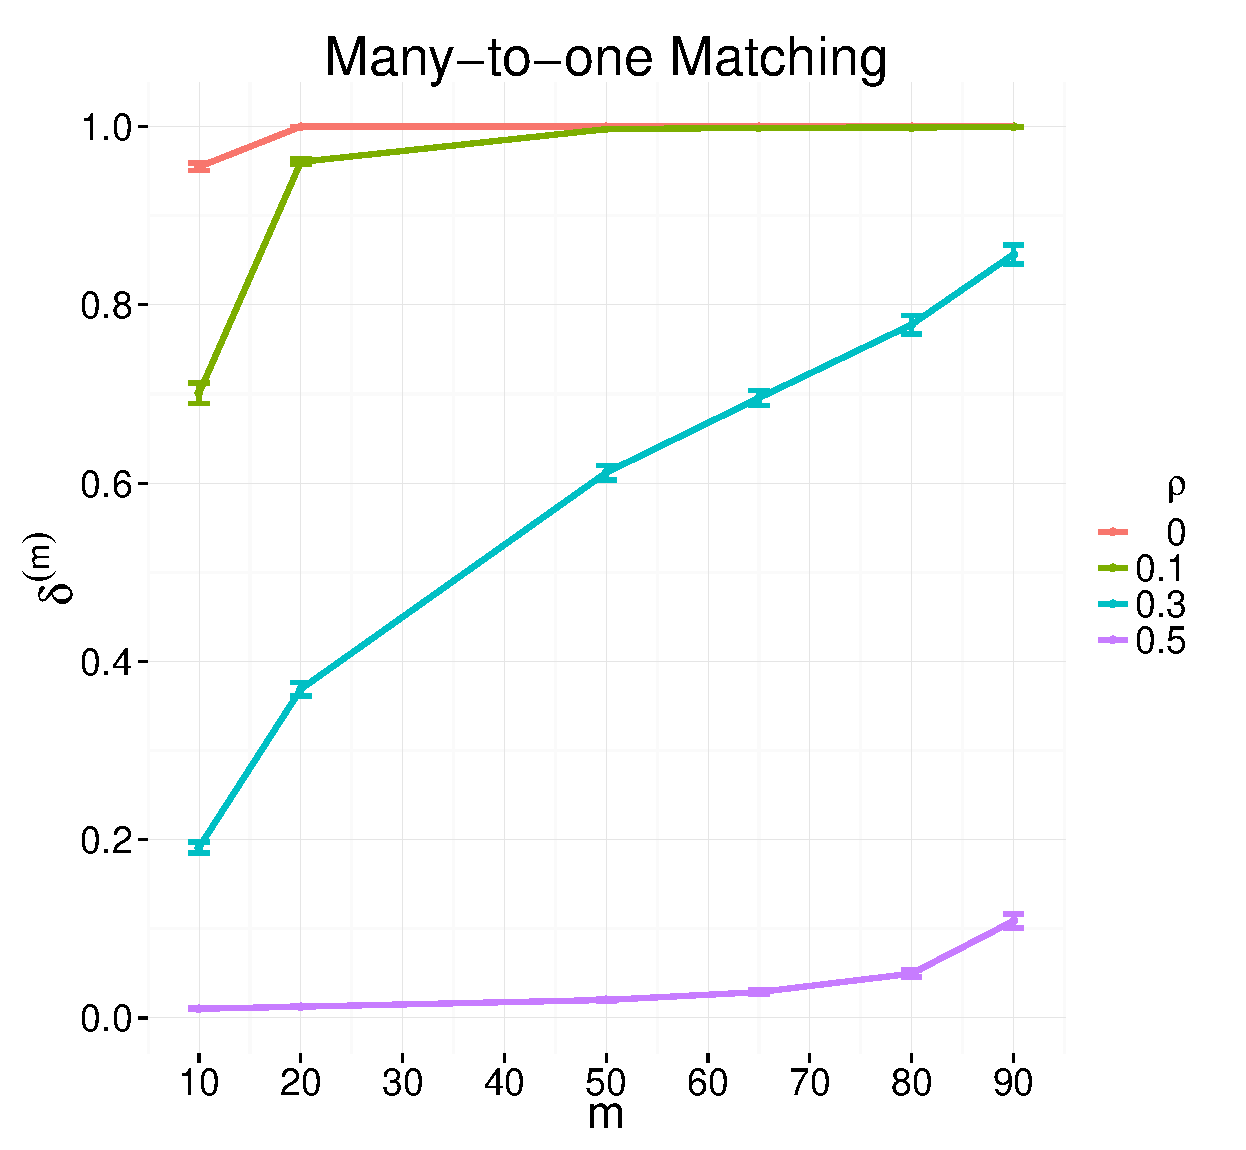
\includegraphics[scale=0.65]{Total_precision_JOFC_1_to_k_match_paper.pdf}
\caption{Graph Matching experiments on simulated graphs for JOFC \label{1_k_graphmatch_sim}}
\end{figure}

The results provide evidence that JOFC is a suitable method for solving this variation of graph matching problem. While  both JOFC and modified FAQ were acceptable solutions for the approximate graph matching (AGM) problem with one-to-one correspondence between vertices, with comparable matching performance, modified FAQ  cannot directly solve  the one-to-$k$ correspondence variation of the GM problem. In contrast, JOFC is quite adequate for solving AGM with one-to-$k$ correspondence. One only needs to use a matching algorithm that allows multiple assignments for the vertices of one of the graphs. We should mention we use the full matching algorithm implemented in R package \cite{optmatch} which finds  `` a matching between units that minimizes the average within grouped distances, given a matrix describing the distances between two groups''\cite{optmatch_manual}. That is, the \emph{full} matching algorithm finds an assignment for all of the vertices in both graphs. As the assignment problem is independent of the embedding, other matching algorithms can be used with the same embedding.



\chapter{Conclusion}
\label{sec:conclusion}
\chaptermark{Optional running chapter heading}

\section{Conclusion}
\subsection{Future Directions}



\include{appendix}

%% REFERENCES

% if you use BIBTEX
\bibliographystyle{IEEEtran}
\bibliography{priebe-thesis-JOFC}
% 
% \begin{vita}
% 
% \begin{wrapfigure}{l}{0pt}
% 
\includegraphics[width=2in,height=2.5in,clip,keepaspectratio]{rjvheadshot}
% \end{wrapfigure}
% 
% 
% 
% \end{vita}
\end{document}
